% !TEX TS-program = xelatex
% !BIB program = bibtex
% !TEX encoding = UTF-8 Unicode
% !Mode:: "TeX:UTF-8"
 \documentclass[bachelor, nocolorlinks, printoneside]{seuthesis} % 本科
% \documentclass[master]{seuthesis} % 硕士
% \documentclass[doctor]{seuthesis} % 博士
% \documentclass[engineering]{seuthesis} % 工程硕士
\usepackage{CJK,CJKnumb}
\usepackage{amsmath}
\usepackage{amsfonts} 
\usepackage{bm} 
\usepackage{algorithm}
\usepackage{algorithmicx}
\usepackage{algpseudocode}
\usepackage{stmaryrd}
\usepackage{placeins}
\usepackage{makecell}
\usepackage{graphicx,subcaption}
\usepackage{booktabs}
\newtheorem{theorem}{定义}
\usepackage{xcolor}
%\usepackage{algorithm,algpseudocode}

\newcommand\TODO[1]{\textcolor{blue}{#1}}

\floatname{algorithm}{算法}
\renewcommand{\algorithmicrequire}{\textbf{输入:}}
\renewcommand{\algorithmicensure}{\textbf{输出:}}
 % 这里是导言区

\begin{document}
\categorynumber{000} % 分类采用《中国图书资料分类法》
\UDC{000}            %《国际十进分类法UDC》的类号
\secretlevel{公开}    %学位论文密级分为"公开"、"内部"、"秘密"和"机密"四种
\studentid{04216747}   %学号要完整,前面的零不能省略。

\title{基于深度学习的三维重建和点云生成}{}{SEU Thesis \LaTeX Template}{subtitle}
\author{周烨凡}{Yefan Zhou}
\advisor{杨绿溪}{教授}{No Name}{Prof.}
\department{信息科学与工程学院}{Radio}
\major[12em]{信息工程}
\duration{2020年1月-2020年5月}

%\advisor{无名氏}{教授}{No Name}{Prof.}



\maketitle

\begin{abstract}{三维重建,点云,深度学习,数据挖掘}

    单视角三维物体形状重建(Single-view 3D Reconstruction)是三维视觉领域一直以来的核心问题之一。
    由于拟合非线性方程和学习模式的有效性,深度神经网络被期望在重建三维非线性形状的任务中表现出色。
    本课题探究了深度神经网络在三维重建任务中的有效性和内在机制,主要的工作和创新如下:
        
        \begin{enumerate}
            \item[1.] 为了验证基于自编码器架构的深度神经网络在三维重建任务中的有效性,提出采用弱标签信息监督对编码器进行初始化,以及用残差层改进解码器这两种方法优化网络架构。在ShapeNet公开数据集上进行测试,取得了超过基于识别机制的非深度学习方法的理论极限的水平,并
            证明了神经网络在此公开数据集上倾向于执行重建机制而非识别机制。 
            \item[2.] 为了衡量三维数据集的聚类程度,提出了基于亲和传播(affinity propagation)和轮廓系数(silhouette score)的度量指标,该指标得到的量化结果与数据集降维后的可视化结果吻合。
            \item[3.] 提出并通过实验证明了影响三维重建任务中深度神经网络内在机制的主要因素是数据集的本质特征:只有当训练集中的三维形状集有相比于图片集更高的聚类程度的结构时,在这个数据集上训练的深度神经网络才会执行识别机制而非重建机制。
        \end{enumerate}
    最后,本文分析了上述结论对三维重建任务中的数据收集和神经网络训练的指导意义。
    \end{abstract}

\begin{englishabstract}{3D Reconstruction, Point Cloud, Deep Learning, Data mining}
    Single-view 3D reconstruction is one of the elementary tasks in the field of 3D vision. 
    Due to the effectiveness in learning and approximating non-linear function, deep neural networks are expected to perform well on the task of reconstructing 3D non-linear shapes.
    This paper investigates the effectiveness and internal mechanism of deep neural network in 3D reconstruction task. 
    The main contribution and innovation are summarized as follows:
    \begin{enumerate}
        \item[1.] In order to verify the effectiveness of the deep neural network based on auto-encoder architecture in 3D reconstruction task, 
        it proposes to leverage supervision of weak class information to initiate the encoder and improve the decoder with residual layer in order to optimize network architecture. 
        These methods are trained and tested on ShapeNet public dataset and they outperform theoretical limit of the non-learning method based on recognition, 
        and it proves that neural network tend to do reconstruction task instead of recognition task in this dataset。

        \item[2.] Define novel way to measure clustering coefficient of 3D reconstruction dataset based on affinity propagation and silhouette score, the quantitative results of this metric is corresponding to qualitative results of visualization of dataset in low dimension.
        \item[3.] It claims and proves by experiments that the bias of internal mechanism of network 
        is mainly affected by the intrinsic properties of dataset: only when the training set of 3D shapes has a 
        more clustered structure than images, the deep neural networks trained on this dataset become more likely 
        to perform recognition than reconstruction.
    \end{enumerate}
    Finally, this paper analyzes the significance of the above conclusions for data collection and neural network training.
\end{englishabstract}

\tableofcontents



\begin{Main} % 开始正文

\chapter{绪论}

\section{课题的背景和意义}
基于单视角二维图片输入进行三维物体形状重建是三维视觉领域的核心问题之一,它能有效解决现实世界中二维数据丰富而三维数据稀少的问题,满足无人驾驶,智能建造,机器人领域的需求。
如图\ref{fig:civil-modeling},在智能建造领域的城市三维建模中,大规模应用该技术将高清航拍获取的RGB图片数据\ref{fig:civil-plane-image}
重建为三维立体数据\ref{fig:civil-recon},结合雷达获取的遥感点云数据\ref{fig:civil-remotesense},
进行高精度的城市建模\ref{fig:civil-high}。点云数据具有易处理,易存储,易获得的特点,
因此成为三维重建研究中常用的三维数据表示之一。

\begin{figure}
	\begin{subfigure}[t]{0.30\linewidth} \centering 
        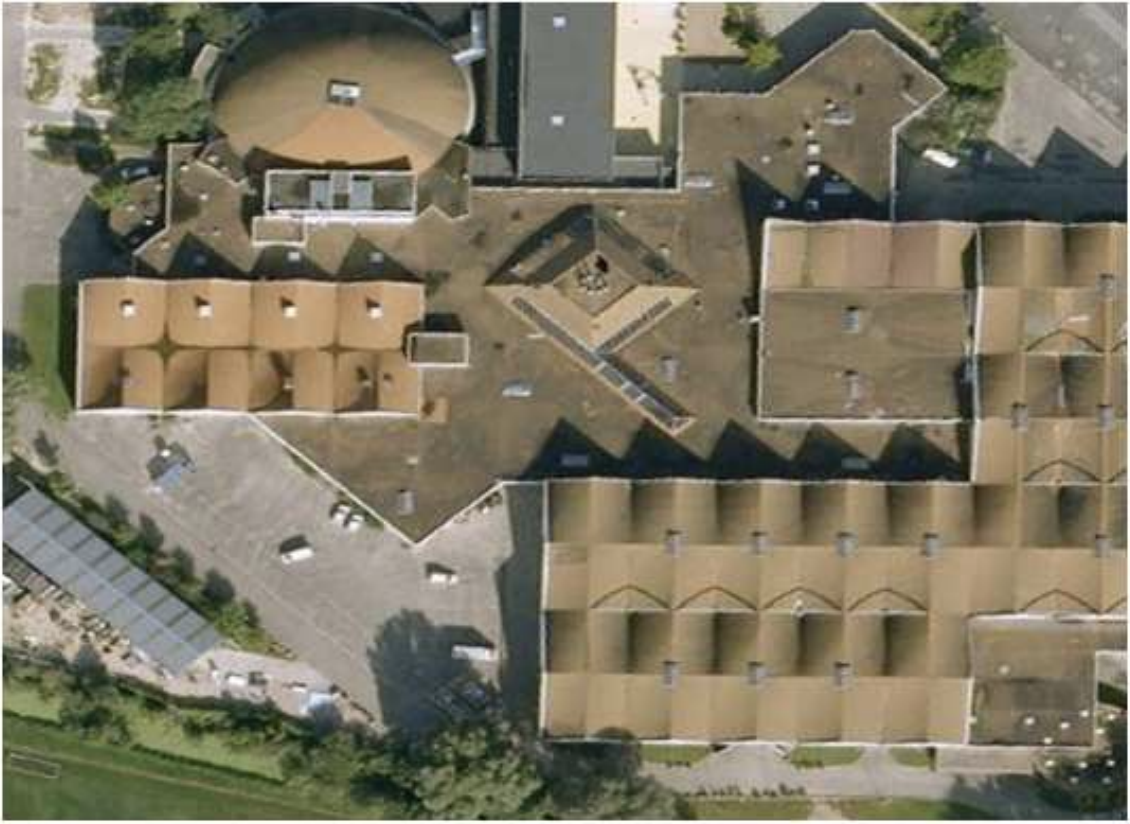
\includegraphics[width=\columnwidth]{figs/app/image.png}
        \caption{高清航拍图片}\label{fig:civil-plane-image}
    \end{subfigure}
    \begin{subfigure}[t]{0.30\linewidth} \centering
        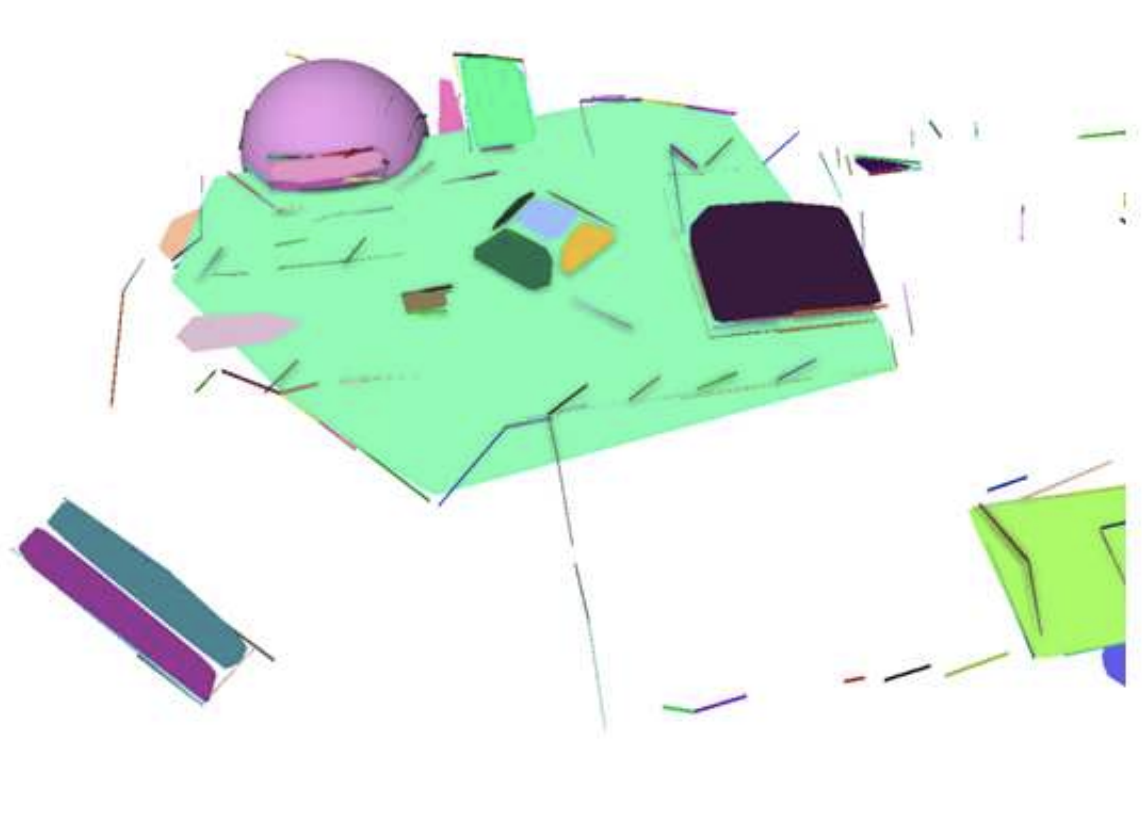
\includegraphics[width=\columnwidth]{figs/app/recon.png}
        \caption{单视角三维重建模型}\label{fig:civil-recon}
    \end{subfigure}
%    \hspace{0.05\linewidth}
    \begin{subfigure}[t]{0.30\linewidth} \centering
        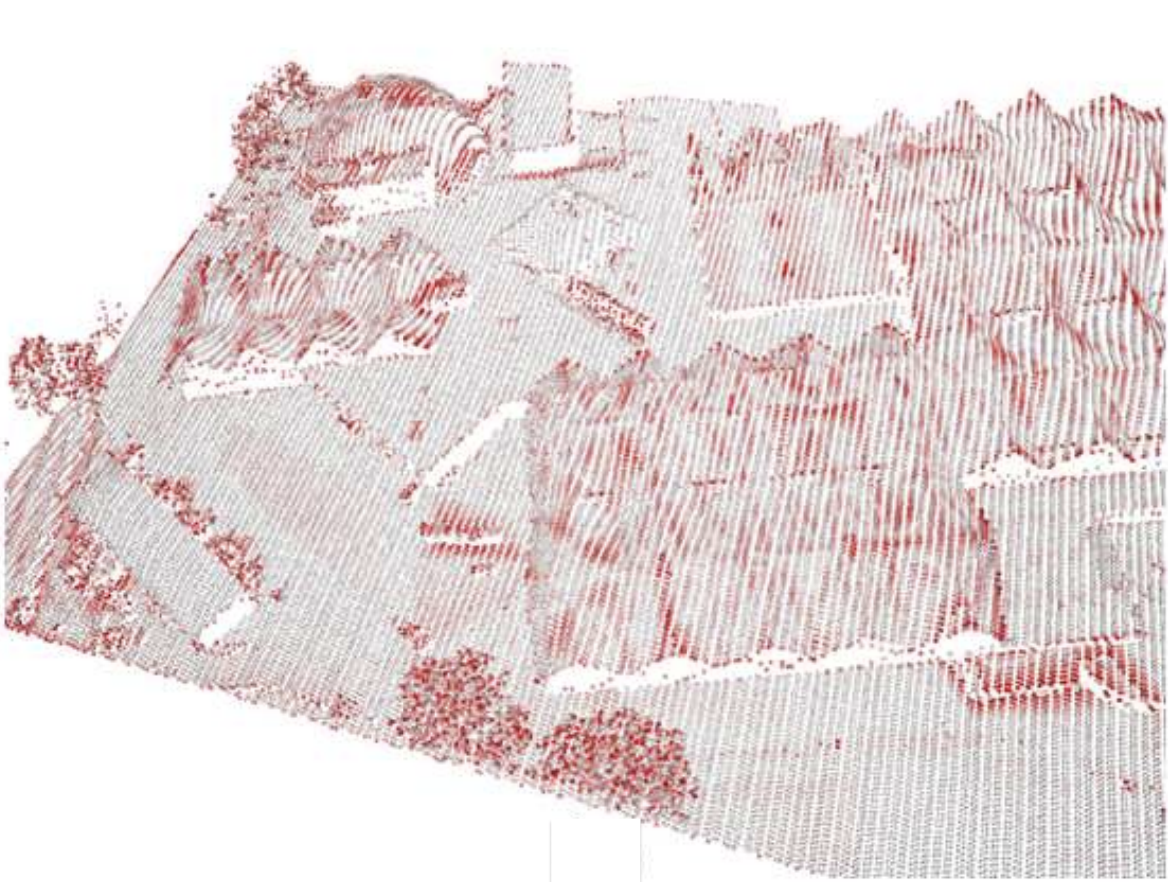
\includegraphics[width=\columnwidth]{figs/app/remotesense.png}
        \caption{遥感点云数据}\label{fig:civil-remotesense}
    \end{subfigure}
    \begin{subfigure}[t]{0.45\linewidth} \centering
        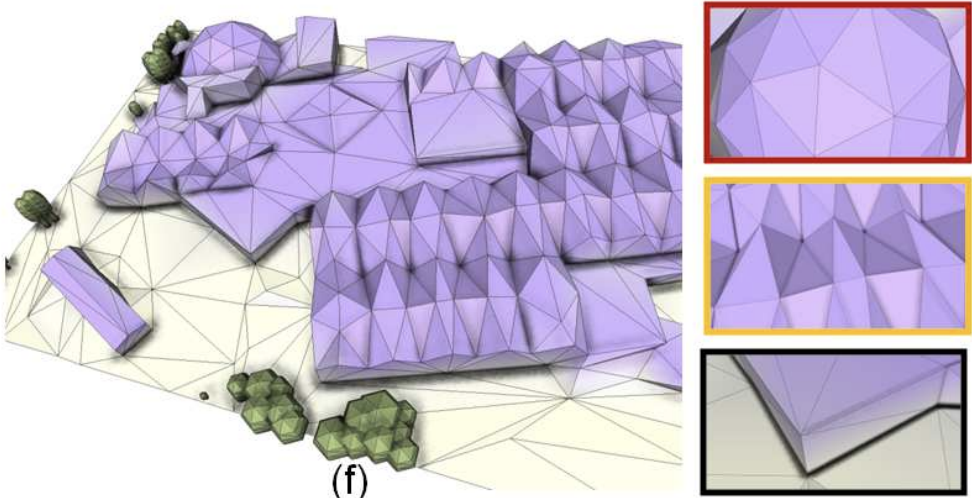
\includegraphics[width=\columnwidth]{figs/app/coarse_modeling.png}
        \caption{低精度建模}\label{fig:civil-coarse} 
    \end{subfigure}
    \begin{subfigure}[t]{0.45\linewidth} \centering
        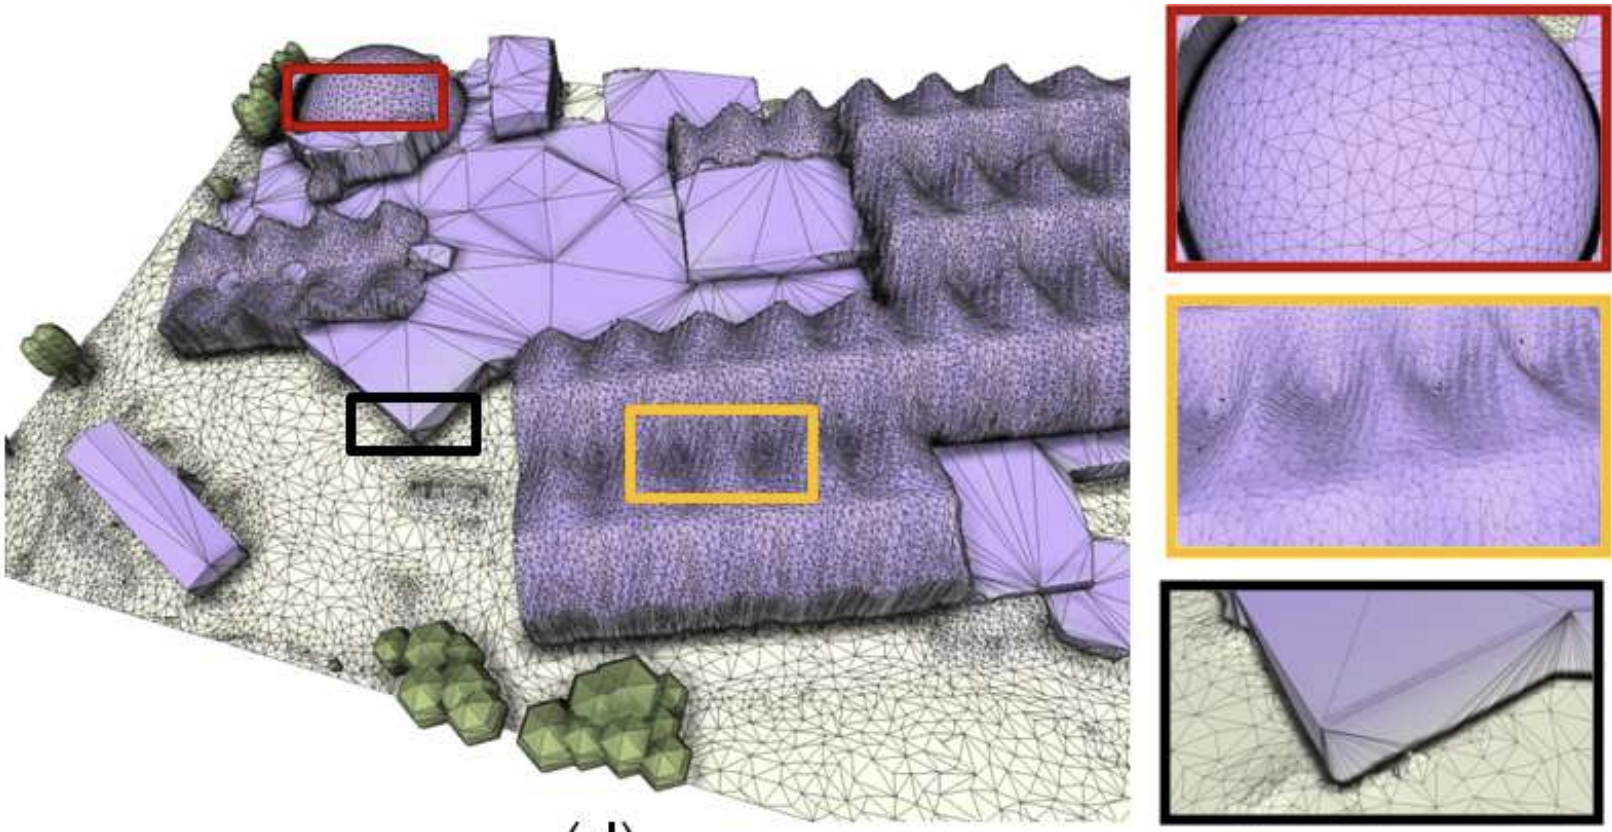
\includegraphics[width=\columnwidth]{figs/app/high_modeling.png}
        \caption{高精度建模}\label{fig:civil-high} 
    \end{subfigure}
  \caption{\small 应用单视角三维重建技术的城市建模 }\label{fig:civil-modeling}
\end{figure}
\FloatBarrier

使用深度学习来进行单视角三维重建持续受到人们的关注。尽管很多的文章已经展示了创新的深度学习框架来提高三维重建任务中的最高水平\cite{li2018point,park2019deepsdf,fan2017point,tatarchenko2017octree,groueix2018papier,yang2018foldingnet,wang2018pixel2mesh,sun2018pix3d,tulsiani2017multi,wu2017marrnet,yan2016perspective},
但很少有文章来尝试探究这些任务的本质特性。不可否认的是,重建三维非常规形状的问题已经变成了一个新的机器学习范例, 
并且从事者使用的处理数据和训练网络的方法与在常规数据上的学习使用的方法不同(比如,Adam\cite{kingma2014adam}的使用频率比SGD要高)。
因此,这引发了研究者对其内在机制的思考,即神经网络在三维重建学习这个新范例上怎样进行学习?是否与传统的向量分类和回归问题不同?

最近, 文章\cite{tatarchenko2019single}的作者针对上述问题提出了一个让人惊讶的观点。
他们尝试性的展示了当前最先进的用于三维重建任务的深度神经网络更倾向于通过首先分类输入图片到一个特定的簇,
然后生成对应簇的平均三维形状,以此来进行预测。支持这一观点的主要实验证据是这些深度神经网络的三维预测结果与纯粹基于聚类和基于检索的基准模型的三维预测结果效果相近。
这是一个非常有趣的观察,因为它说明了对于三维重建的任务来说,深度神经网络倾向于记住平均形状并且将其与图片输入的语义联系起来,而不是使用几何方法来生成一个形状,
比如通过融合细粒度的局部结构形成一个整体形状。如果这个观点是正确的,这说明对于三维重建任务来说,
最先进的深度神经网络实际执行了一个记忆任务而不是一个泛化任务\cite{arpit2017closer}。

本课题旨在优化三维重建任务中深度神经网络的架构,证实其有效性。
同时进一步探究深度神经网络在三维重建任务中的内在机制,分析导致其偏倚于识别或重建机制的因素,
这一研究将会帮助当前应用于三维重建的深度学习方法避免陷入识别机制的误区,同时也探讨了深度学习的本质问题,
即如何帮助神经网络进行更好的泛化。



\section{研究现状}
\subsection{相关模型}
PSGN\cite{fan2017point}的作者首次提出了以单张图片作为输入的三维点云重建任务中深度神经网络的基本架构, 
即自编码器架构。编码器由卷积层和ReLU层构成,编码器的输入是一张图片和一个向量,向量用来模拟重建任务中的不确定性。
解码器由全连接层构成,解码器输出点云的坐标,用 N × 3 的矩阵表示,N 为一个点云中三维点的数量。
FoldingNet\cite{yang2018foldingnet}的作者提出了以三维点云作为输入的三维点云重建任务中深度自编码器的架构,
创造性的提出用折叠的思想来生成点云,并重建三维形状,根据该思想实现的解码器仅使用了全连接层解码器的7\%的参数量,
却在重建效果上超过当时的基准模型。
文章\cite{tatarchenko2019single}中评估了多个效果拔尖的单视角三维重建深度神经网路模型,
并提出了基于识别和检索机制的多个非深度学习方法模型,且这些模型的重建性能超过了
当前的深度学习网络模型,这使得深度学习在单视角三维重建中的有效性受到了置疑。

\subsection{相关数据集}
ShapeNet\cite{chang2015shapenet}是一个注释丰富且规模较大的三维形状数据集,涵盖55个常见的类别,有大约5万个样本,
每个样本内有一个三维模型和多张从不同视角渲染的该三维模型的图片,三维模型的数据格式为网格、体素,图片格式为PNG,
在进行单视角三维重建时会从多个视角图片中选择一个视角的图片,因此这种情况下每个样本内有一张图片与一个三维模型。
该数据集的创立者在ICCV 2017 举办了基于该数据集的单视角三维重建任务的竞赛,并将当时的基准成绩发表在论文\cite{Yi2017LargeScale3S}中。
论文\cite{tatarchenko2019single}提供的数据集在ShapeNet\cite{chang2015shapenet}的基础上增加了点云数据格式,
每个三维形状由9000多个点构成。共有52430个样本,涵盖55个类。

\subsection{神经网络学习机制}
深度神经网络是执行记忆还是泛化一直是现代机器学习中的主要问题。与我们将要介绍的类似,众所周知的猜测是优化过程是“内容感知”的,
并且取决于数据本身的属性\cite{arpit2017closer}。该论文\cite{arpit2017closer}中还显示,
训练期间的某些正则化技术可帮助深度神经网络泛化而不是记住任务。对于三维形状重建,\cite{tatarchenko2019single}表明神经网络倾向于记忆平均形状,
而不是在几何意义上进行重建。确实,许多作品还显示了平均形状和识别信息在提高三维重建效果中的有效性\cite{kanazawa2018learning,pontes2018image2mesh,kurenkov2018deformnet}。

相比之下,也有很多作品利用三维形状的连续潜在空间中的分布信息\cite{li2018single,gwak2017weakly,sinha2017surfnet,li2018point,wu2018learning,yang20173d,yang2019pointflow}来提高三维重建效果,
这超出了基于识别的范围。值得注意的是,相关工作\cite{wu2016learning,girdhar2016learning}表明形状算术可以在三维形状的潜在空间中进行,
从而排除了神经网络仅在此问题设置中执行识别的可能性(因为执行算术需要的不是均值信息离散簇的形状)。
其他一些工作建议通过将每个形状分解为部分\cite{tulsiani2017learning,niu2018im2struct,sung2017complementme}或通过连续过程\cite{sun2018pointgrow,choy20163d}来生成三维形状,
这也超出了简单的识别任务。但是, 相关论文\cite{wu2016learning,achlioptas2017learning,yang2018foldingnet}的作者将基于三维重建的自动编码视为点云上无监督分类的基础。
尽管这些作品中的输入数据是三维形状,而不是二维图像,但是形状信息有助于分类的事实似乎确实增强了这样的概念,即三维重建更着重于识别而不是重建。
尽管如此,形状信息有助于识别的事实不能成为判断三维重建网络所学知识的主要理由。有意义的未来方向是研究分别用于无监督分类和受监督三维形状重建的神经网络学习之间的差异,因为这两个方向的主要目标并不完全相同。

注意三维重建问题可以被看作是一个更普适的分布学习\cite{oliva2013distribution,poczos2013distribution}的特殊情况。但是,与分布学习中的理论工作如拓展核方法到回归分布不同,我们的工作集中于深度学习。即便如此,使人感兴趣的是能看到分布学习的传统工作把输出分布当做一个所有训练分布样本的连续线性组合直接处理,而不是使用两步法,预测簇索引后再预测平均分布。
\section{本文研究内容}
\subsection{课题关键问题以及难点}
首先,正式定义本课题的关键问题:一、优化深度神经网络框架,使其在单视角三维重建任务中超过基于识别机制的非深度学习方法,证明其有效性。二、讨论深度神经网络在单视角三维重建任务中执行的是识别机制还是重建机制。初步猜想是影响其在两者之间偏倚的因素为训练数据集的整体特征:聚类程度。因此本课题需要考虑以下几个难点:
\begin{enumerate}
    \item[1.]改进当前作为基准的神经网络架构以获得更好的重建性能。我们希望能对当前作为基准线的深度神经网络进行架构优化,以期望其在公认的标准数据集上能接近并超越基于识别机制的非深度学习方法。因此我们考虑借鉴图像领域成熟且有效的神经网络架构优化方法和训练技巧。
    \item[2.]定义神经网络的识别与重建这两种机制的数学表达,并用具体的实验结果来描述。
    \item[3.]设计并产生具有量化特征的三维重建数据集。为了探究神经网络训练集和网络的性能之间是否有强相关性,需要能定量的操控数据集的某些整体特征,如聚类系数。可以考虑的方式就是生成自定义的数据集,同时在生成过程中通过采样改变整体特征。为此可以考虑使用计算机图形学的相关软件来合成三维模型,并探究一些能进行不同三维形状之间插值形变的算法。
    \item[4.]定义衡量数据集指标的度量标准。在解决问题三后,需要构建一个度量标准来衡量数据集的聚类趋势,得到量化评分。   
\end{enumerate}

\section{论文组织结构}
本论文主要有六个章节,各章的内容安排如下:
\begin{itemize}[\hspace{2cm}]
    \item[第一章] 绪论,简要介绍了单视角三维重建任务的研究背景和意义,并对现行的相关理论,模型和数据集进行简单概述与分析。介绍本论文的研究思路、关键问题以及主要贡献。
    \item[第二章] 问题与定义,介绍了本论文探究的损失函数和算法的理论基础。给出了重建机制与识别机制的数学定义。
    \item[第三章] 模型方法,详细介绍了基准模型,以及优化模型的架构,并给出了网络在ShapeNet大型数据集上训练的过程信息以及训练结果的分析比较。
    \item[第四章] 机制分析,给出了机制探究的理论基础与实验设计,介绍了自定义数据集的制作,网络在自定义数据集上训练的过程信息以及训练结果的定性与定量分析。
    \item[第五章] 总结与展望,分析并总结本课题研究成果的总体优缺点,并提出未来的研究方向。
\end{itemize}


\chapter{问题与定义}
\section{问题描述}
我们探究的问题是从单张图片输入重建一个三维形状。输入$I$是一张二维RGB图片。输出$S$由一个点云表示。我们在本文中不考虑基于体素的体积表达。对于基于点云的表达,
每个形状$S$是一个包含三维点的点集。一个神经网络在训练中通过减小特定损失函数定义的经验损失$l$,以此来从输入图片$l$预测形状$S$,该过程的数学定义为:
\begin{equation}
    \min_f \sum_{i=0}^{n-1} {l(f(I_i), S_i)}.
\end{equation}
我们想通过优化模型$f$,使其在训练数据集上训练后,在测试数据集上取得更低的平均损失。同时,我们还想学习$f$的特性来了解它执行的是一个重建任务还是识别任务。
两个指标被用来测量重建结果$\widehat{S} = f(I)$与标签点云$S$之间的差异,称为Chamfer Distance和F-score。
\\
\noindent
\textbf{Chamfer distance.}\label{sec:chamfer}~~Chamfer Distane通过搜索另一个点集中最近点来测试一个点集到另一个点集的整体距离。
\begin{equation}\label{eqn:chamfer}
	d_{CH}(S,\widehat{S}) = \frac{1}{|S|}\sum\limits_{\mathbf{x}\in S}\min_{\widehat{\mathbf{x}}\in \widehat{S}}\|\mathbf{x}-\widehat{\mathbf{x}}\|_2 + 
    \frac{1}{|\widehat{S}|}\sum\limits_{\widehat{\mathbf{x}}\in \widehat{S}}\min_{\mathbf{x}\in S}\|\widehat{\mathbf{x}} - \mathbf{x}\|_2.
\end{equation}
尽管Chamfer Distance是运算高效且方便的,它受到很小一部分异常点的影响强烈。所以我们也要如文章\cite{tatarchenko2019single}建议的那样采用F-score来预测点集。
\\
\noindent
\textbf{F-score.}\label{sec:fscore}~~另外一个衡量形状重建的指标是F-score, 该指标是精确度和回忆度的调和平均数。在给定相应的标签点云$S$,且在固定的距离阈值$d$内,重建点云$\widehat{S}$
的精确度$\textit{Prec}$被定义为:

\begin{equation} \label{eq:precision}
\textit{Prec}(\textit{d}, S, \widehat{S}) = \frac{1}{|\widehat{S}|} \sum_{r \in \widehat{S}} \llbracket \min_{s \in S} ||r-s || < \textit{d} \rrbracket,
\end{equation}
其中$\llbracket \cdot \rrbracket$ 是艾佛森括号。
    
相似的,标签点云$S$对重建点云$\widehat{S}$的回忆度$\textit{Rec}$是:
\begin{equation} \label{eq:recall}
    \textit{Rec}(\textit{d}, S, \widehat{S}) = \frac{1}{|S|} \sum_{s \in S} \llbracket \min_{r \in \widehat{S}} ||s-r || < \textit{d} \rrbracket.
    \end{equation}
其中$\llbracket \cdot \rrbracket$ 是艾佛森括号。

由$Prec$和$Rec$,如下计算F-score:
\begin{equation} \label{eq:f-score}
    \textit{F}(\textit{d}, S, \widehat{S}) = \frac{2 \times \textit{Prec}(\textit{d}, S, \widehat{S})\times \textit{Rec}(\textit{d}, S, \widehat{S})}{\textit{Prec}(\textit{d}, S, \widehat{S}) + \textit{Rec}(\textit{d}, S, \widehat{S})}.
\end{equation}
重建的准确度被精确度量化,用以测量重建点集和标签点集的距离。重建的完整度被回忆度量化,用来测量标签点云多少部分被重建点云覆盖。
所以,一个高的F-score显示了重建是准确且完整的\cite{knapitsch2017tanks}。
\section{识别机制和重建机制}
\label{sec:recog_or_recon}
在这个部分,我们正式定义本文中研究的两种学习范式,被称为识别(\emph{recognition})和重建(\emph{reconstruction})

\begin{theorem}\label{def:recognition}(识别)
    一个基于识别机制的神经网络$f$用两步预测形状重建。神经网络重建方程可以写成:
\begin{equation}
        \widehat{S} = f(I) = f_1(f_2(I)),
\end{equation}
方程中的$f_2(\cdot)$将输入图片映射到一个标量索引,并且$f_1(f_2(I))$将这个标量索引映射到索引$f_2(I)$对应的特定簇的平均形状。
\end{theorem}

\begin{theorem}\label{def:reconstruction}(重建)
    一个基于重建机制的神经网络直接进行三维重建。即\begin{equation}
        \widehat{S} = f(I),
    \end{equation}
并且重建不会明显的使用图片簇的任何信息。
因为当前最常见的单视角三维重建经常使用一个”编码器-解码器”结构,所以一个相似的概念是由编码器获得的码字不会形成簇。
\end{theorem}
\textbf{主要问题}

在这篇论文中,我们研究神经网络执行识别机制还是重建机制。我们展示了在两者之间偏倚的趋势由数据集特性决定。

值得注意的是论文\cite{tatarchenko2019single}的主要结论是单视角三维重建中的深度神经网络主要执行识别工作。换句话说,该论文的观点是神经网络的方程更接近于定义\ref{def:recognition}而不是
定义\ref{def:reconstruction}。
\section{数据集的聚类趋势}
\label{sec:metric_on_dataset}
在这个部分,我们定义用来测量数据集聚类趋势的指标。具体来说,我们使用silhouette score\cite{van2015using}来测量聚类趋势。
给定一个数据集$D = \{x_i\}_{i=0}^{N-1}$和一个随机距离$d(x,y)$方程\footnote[1]{我们考虑满足下面三个属性的任何距离方程,
$d(x_1,x_2)=d(x_2,x_1)$, $d(x_1,x_2)\ge 0$, 和 $d(x,x)=0$。在我们的实验中,我们使用Chamfer Distance作为点云的距离指标。
我们使用$\ell$-1距离作为图片之间的距离。}。我们能通过明确一个聚类特性方程$C(\cdot)$来确定一个数据集的簇。对于每个样本$x_i$,
聚类方程会给出一个聚类标签$C(x_i)$。我们使用$C(x_i)$来指示包含有$x_i$的簇,比如说,聚类标签$C_i$等价于$C(x_i)$。有时候,数据集
已经包含了标签聚簇划分。更多情况下,聚簇划分需要通过一个算法来获得。然后,第$i$个样本的轮廓系数(silhouette score)被定义为:
\begin{equation}
    s(i) = \frac{b(i)-a(i)}{\max(a(i),b(i))},
\end{equation}
其中
\begin{equation}
    a(i) = \frac{1}{|C_i|-1}\sum_{j\in C_i, j\neq i}d(i,j),\;\;\;\;\;
    b(i) = \min_{k\neq i}\frac{1}{|C_k|}\sum_{j\in C_k}d(i,j).
\end{equation}
聚类趋势, 以轮廓系数定义, 由以下方程得出:
\begin{equation}
    \textit{Clustering-tendency} = \frac{1}{N}\sum_i s(i).
\end{equation}

对于没有标签聚类的数据集,我们需要找到聚类方程$C(\cdot)$。在这篇论文中,我们使用亲和传播(affinity propagation)\cite{wang2008adaptive}
来进行聚类。亲和传播非常适合我们的设定,因为它不需要预先确定簇的数量,并且它使用一个预设的距离矩阵来
分配数据点$x_i$到一个簇$C_i$。我们使用Chamfer Distance\eqref{eqn:chamfer}作为距离方程$d(x,y)$来处理
数据集中的无序点云。

\subsection{亲和传播}
亲和传播(Affinity propagation)是一个基于数据点消息传播理论的聚类算法。亲和传播在运行算法之前不需要预先设定簇的数量,
而是通过反复迭代从输入数据集中选出“示例(exemplars)”来代表一个簇。

给定一组数据点从$x_1$到$x_n$,先根据预先定义的距离方程计算距离矩阵,再将距离矩阵取负后转化为相似度矩阵(Similarity matrix)。在这个基础定义处,我们
使用欧式距离作为距离方程,相似度矩阵可以被写为:
\begin{equation}
    s( i , k)= -|| x_i - x_j ||^{2}
\end{equation}

亲和传播以相似度矩阵作为输入进行无监督训练,
在运行过程中我们需要考虑这几个矩阵:责任矩阵(Responsibility matrix),获取度矩阵(Availability matrix),
规则矩阵(Criterion matrix)。算法在运行过程中对这几个矩阵进行如下更新:

首先责任矩阵$r(i,k)$量化了第$k$个元素适合成为第$i$个元素的示例的程度,并考虑了最近的竞争者第$k^{'}$个元素可能成为第$i$个元素的示例这个因素。
\begin{equation}\label{eqn:resp_matrix}
    r(i, k) \leftarrow s(i, k)-\max _{k^{\prime} \neq k}\left\{a\left(i, 
k^{\prime}\right)+s\left(i, k^{\prime}\right)\right\}
\end{equation}

接着获取度矩阵的非对角线元素$a(i,k)$量化了第$i$个元素选择第$k$个元素作为示例的合适程度,考虑了其他元素支持k成为一个示例的程度。

\begin{equation}\label{eqn:avail_matrix}
    a(i, k) \leftarrow \min \left(0, r(k, k)+\sum_{i^{\prime} \notin\{i, k\}} \max \left(0, r\left(i^{\prime}, k\right)\right)\right) \text { for } i \neq k
\end{equation}

获取度矩阵的对角线元素$a(k,k)$反映了第$k$个元素适合成为一个示例的累积证据,基于k对于其他元素的积极责任。
\begin{equation}\label{eqn:avail_matrix_dia}
    a(k, k) \leftarrow \sum_{i^{\prime} \neq k} \max \left(0, r\left(i^{\prime}, k\right)\right)
\end{equation}

责任矩阵与获取度矩阵被运算\ref{eqn:resp_matrix},\ref{eqn:avail_matrix},\ref{eqn:avail_matrix_dia}迭代更新,这个过程也许在一定的
迭代步骤之后停止,也许在这两个矩阵的值收敛后停止。停止后,我们计算规则矩阵$c(i,k)$:
\begin{equation}
    c(i, k) \leftarrow r(i, k)+a(i, k)
\end{equation}

每行中具有最高标准值的元素将被指定为示例。与该示例的标准值相同的行对应的元素被划分为同一集群。
%\begin{algorithm}
%    \caption{Affinity Propagation}
%    \label{alg:affinity}
%    \begin{algorithmic}[1] %每行显示行号
%        \Require $s(i,k)$相似度矩阵
%%        \Ensure $c(i,k)$规则矩阵
%        \State $Initiate a(i,k) \gets 0$
%        \State $Initiate r(i,k) \gets 0$
%        \Repeat
%        \State $r(i,k) \gets s(i,k) - $
%        \Until{convergence}
%    \end{algorithmic}
%\end{algorithm}

\chapter{模型方法}
在这个部分,我们介绍了本文研究的三维重建任务中深度神经网络基准模型和非深度学习基准模型,并结合在ShapeNet上的实验结果对其优缺点进行分析。
基于这些分析,对深度神经网络基准模型进行优化,使其超过基于检索机制的非深度学习基准模型,证实了深度
学习的优越性,我们使用了这两种方法:
\begin{itemize}[\hspace{1cm}]
    \item[1.] 引入弱标签信息进行多任务训练
    \item[2.] 使用残差层改进解码器结构
\end{itemize}
我们还展示了在真实数据集ShapeNet上,即使是一个标准的三维重建深度神经网络也倾向于执行重建任务而不是识别任务。我们
的结论基于两点观察:
\begin{itemize}[\hspace{1cm}]
    \item[1.] 标准的三维重建网络获得的重建结果在量化指标如Chamfer Distance和F-score上超过了基于识别机制的分类器的理论极限(Oracle-Nearest-Neighbor)。
    \item[2.] 由自编码训练获得的高维码字的二维 T-SNE 可视化,和使用标签信息进行训练相比,并没有展示出明显的形成簇的趋势。
    而且,没有标签的重建效果比有标签的重建效果要更好。
\end{itemize}

在这个章节,我们使用的数据集均为ShapeNet, 共计55个类,52430个样本,训练集~/~验证集~/~测试集按照70\%~/~10\%~/~20\%随机采样划分。图片大小为$224 \times 224 $,
每个三维点云有1024个三维点构成。


\section{基准模型}
\subsection{模型介绍}
\subsubsection{非深度学习方法}

论文\cite{tatarchenko2019single}中提出了以下三个基于识别机制的非深度学习模型:
\begin{itemize}
    \item \textit{Clustering}:通过对样本点云集使用聚类算法,将一组点云集划分为多个集群,每个集群内部计算一个平均
    三维形状,接着训练一个基于输入图片预测特定集群的分类器,将集群的平均三维形状作为预测结果。
    \item \textit{Retrieval}:借鉴了现有的基于图片检索对应物体的三维形状的方法\cite{10.1145/2816795.2818071},在测试
    时,根据输入图片检索训练集中对应的三维点云,直接提取出来作为预测结果。
    \item \textit{Oracle-Nearest-Neighbor\footnote[1]{下文缩写为Oracle-NN}}:该模型在预测时,在训练集中直接搜索与标签点云损失最小的训练点云,将其
    作为预测结果。因为该模型在进行搜索时需要提供不应该获得的标签点云,而实际测试时只有对应的二维图片作为输入,所以在实践中是不可能
    应用的。
\end{itemize}

因为论文\cite{tatarchenko2019single}的实验结果表明Oracle-NN的水平超过了所有当前最先进的
深度学习模型,而且它是表征任何实际基于识别(检索)机制的非深度学习方法的性能极限的理论基准。所以我们将其当做本课题的非深度学习基准模型, 并进行如算法\ref{alg:orcalenn}的实现。
我们发现在将该模型应用到ShapeNet时,因为测试集有10000个样本,训练集有35000个样本,如果直接应用,复杂度很高,需要在GPU上消耗大概一周时间,占用了大量的计算资源。
于是考虑利用数据集自带的类标签,共计55个类,如车,床,椅子等,在每个类内数据集中运行该算法\ref{alg:orcalenn},大约10小时完成。

\begin{algorithm}
    \caption{Oracle Nearest Neighbor}
    \label{alg:orcalenn}
    \begin{algorithmic}[1] %每行显示行号
        \Require ${T^{n}_{i=0}}$测试集,${D^{t}_{j=0}}$训练集
        \Ensure ${R^{n}_{k=0}}$预测结果
        \State $i \gets 0$
        \State $k \gets 0$
        \While{$i<n$}
            \State $index \gets 0$
            \State $mindis \gets inf$
            \State $j \gets 0$
            \While{$j<t$}
                \State $dis \gets Distance(T_i, D_j)$
                    \If{$dis < mindis$}
                        \State $index \gets j$
                        \State $mindis \gets dis$
                    \EndIf
                \State $j \gets j+1$
            \EndWhile
        \State $R_{k=i} \gets D_{j=index}$
        \State $i \gets i+1$
        \EndWhile
    \end{algorithmic}
\end{algorithm}

\subsubsection{深度学习方法}

\begin{figure}
    \centering
    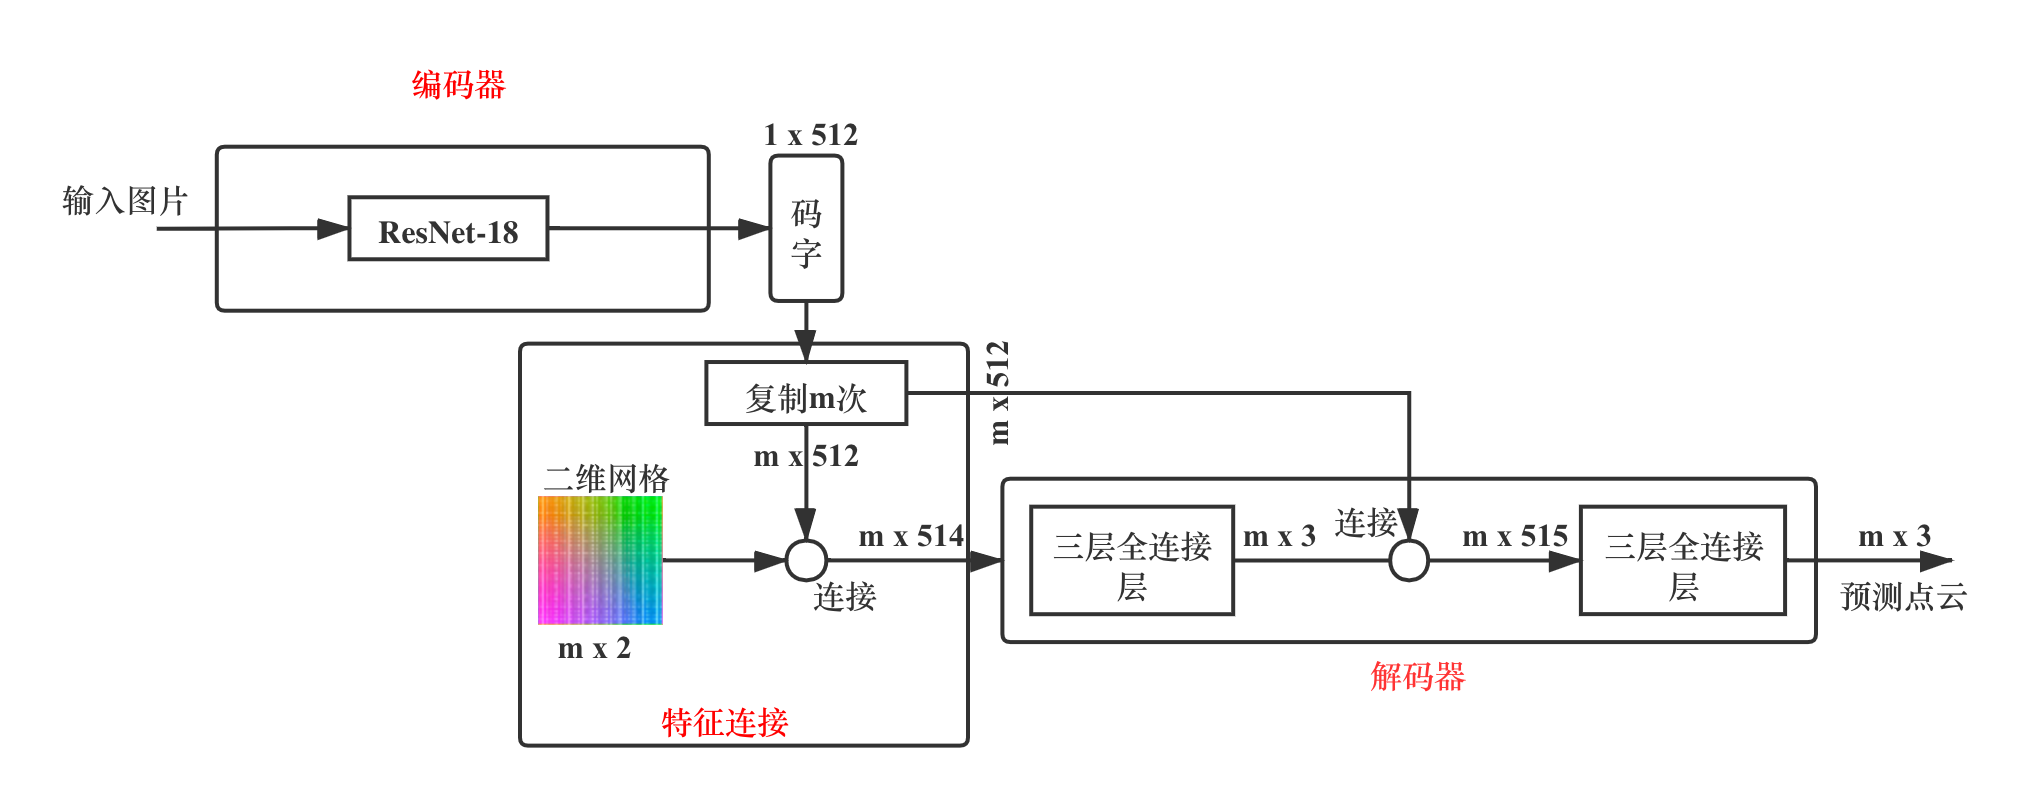
\includegraphics[width=0.99\textwidth]{figs/model/ae_baseline_grid.png} 
    \caption{基于自编码器架构的深度神经网络基准模型}
    \label{fig:ae_baseline}
\end{figure}
根据论文PSGN\cite{fan2017point}提出的基于自编码器架构\footnote[1]{实际为“编码器-解码器”架构,因为输入输出分别是同一个物体的图片与三维点云形状所以简称为自编码器架构}的深度神经网络模型,我们进行了如图\ref{fig:ae_baseline}的实现。网络的主要架构如下:
\begin{itemize}
\item 编码器:采用ResNet-18\cite{He_2016}的卷积层架构作为接受二维图像输入并提取图像特征的编码器, 具体来说,移除ResNet-18最后一层用来分类的全连接层,将一维特征层直接输出作为码字。
\item 特征连接:模型中存储有一个预先初始化好的二维正方形网格点云,长宽在[-1,1]之间,由$m \times 2$的矩阵表示。在将码字输入解码器之前,
我们先将其复制$m$次,然后将$m \times 512$矩阵(码字)与$m \times 2$矩阵(二维网格)连接起来,连接的结果是大小为$m \times 514$的矩阵。
\item 解码器:采用FoldingNet解码器\cite{yang2018foldingnet}作为从码字恢复到点云结构的解码器,具体来说,这个解码器由两个感知器构成,每个感知器由三层全连接层构成。
\end{itemize}

该基准模型的关键是采用了FoldingNet\cite{yang2018foldingnet}提出的解码器架构,使用两个连续的3层感知器将固定的2D网格扭曲为输入点云的形状。这个过程称为折叠操作,实质上形成了通用的二维到三维映射。
为了直观地解释为什么这种折叠操作是通用的二维到三维的映射,用矩阵$U$表示输入的二维网格点。$U$的每一行都是一个
二维网格点。用$U_i$表示$U$的第$i$行,用$\theta$表示编码器输出的码字。然后,在特征连接之后,解码器的输入矩阵的
第$i$行为$[u_i,\theta]$,由于感知器并行应用于输入矩阵的每一行,因此输出矩阵的第$i$行可以写成$f([u_i,\theta])$,其中
$f$表示感知器进行的功能。可以将该函数视为带有码字$\theta$的参数化高维函数,码字$\theta$是指导功能结构(折叠操作)的参数。由于多层感知器
擅长拟合非线性函数,因此它们可以在二维网格上执行精细的折叠操作。本文使用的解码器架构包含有两个感知器模块,第一个模块将二维网格折叠到三维空间,
第二个模块在三维空间内继续折叠网格,使其接近标签形状。

\TODO{可以考虑增加深度神经基准模型的预测结果可视化}
\subsection{实验结果与分析}

在这个部分,我们展示了上述的深度学习基准模型和非深度学习基准模型在ShapeNet上的实验效果,并指出深度学习基准模型的问题。

对于非深度学习基准模型Oracle-NN, 我们展示了所有重建样本的损失平均值作为量化的评估结果。
对于基于自编码器架构的深度学习基准模型,我们以Chamfer Distance\footnote[2]{Chamfer Distance数值越小说明重建效果越好}作为损失函数,使用Adam优化器,训练了100个周期,使其达到收敛,并对超参数进行调参,总共进行了8次训练,最终展示了
由所有重建样本的损失平均值表示的最优重建效果。两个模型的最优结果展示在表\ref{table:metric_per_baseline}。从这个结果中我们可以看出,在最优平均损失方面,Oracle-NN
优于深度神经网络,这一结果与论文\cite{tatarchenko2019single}中展示的两者之间的差距相吻合,而且正如前文所展示的,Oracle-NN是一个理论上的基于识别机制的基准模型,
无法应用于实际任务,所以这一优越结果是被预计的。但是,在训练的过程中,我们发现了神经网络基准模型暴露出的问题,这意味着有可能通过一些架构优化或者训练技巧来继续缩小这一差距。
结合图\ref{fig:lossplot}展示的在不同学习率下深度神经网络的两次训练过程的损失变化\footnote[1]{其他所有超参数如权重损失,动量等均相同}, 对这些问题的分析如下:
\begin{itemize}
    \item 神经网络训练状态不稳定,对初始化要求较高。首先可以看出,在使用Adam优化器的情况下,学习率从0.003到0.01仅增大了三倍,
        就使得网络陷入了与最优效果相差较大的局部最优,且Adam优化器也没有能使得网络跳出这个局部最优点。在正常情况下,网络不应该对超参数有如此高的敏感程度。这也说明重建任务对
        神经网络参数初始化有比较高的要求。
    \item 当前深度神经网络架构学习能力弱,一方面解码器较浅的网络深度可能不足以完成当前复杂的任务。另一方面可能出现了梯度消失的问题,
    如图\ref{fig:testloss}所示,两个网络分别在第30周期和第60周期过早收敛,
    但收敛后的损失仍处于较高水平,这说明当前的网络可能出现了训练过程中梯度消失的问题,导致网络权重难以更新。
    
    \item 神经网络的编码器缺少显性的训练指导。从理论角度来说,网络损失函数仅描述两个三维点云的相似程度,因此有理由怀疑该函数传播的梯度并不能给予对二维图片进行处理的
    编码器足够的优化指导,使其提取需要的图片特征。从实验角度来说,我们将编码器输出的码字进行了二维T-SNE降维可视化,如图\ref{fig:T-SNE2},可以看出
    编码器提取的码字并不具有区分图像类别的特征,虽然这不能证明编码器完全没有提取有助于三维重建的图像信息。
\end{itemize}

基于上述对神经网络基准模型的问题分析,我们将在下文对网络初始化和梯度消失等问题提出优化方案。
\begin{table}
    \centering
    \caption{基准模型的评估结果}
    \label{table:metric_per_baseline}
    \begin{tabular}{cc} 
    \hline
    模型         & Chamfer Distance        \\ 
    \hline
    Oracle-NN  & 0.0719                  \\
    自编码器(基准模型) & 0.0806 \\
    \hline
    \end{tabular}
\end{table}

\begin{figure}[!htb]
    \centering
       \begin{subfigure}[t]{0.49\linewidth} \centering 
         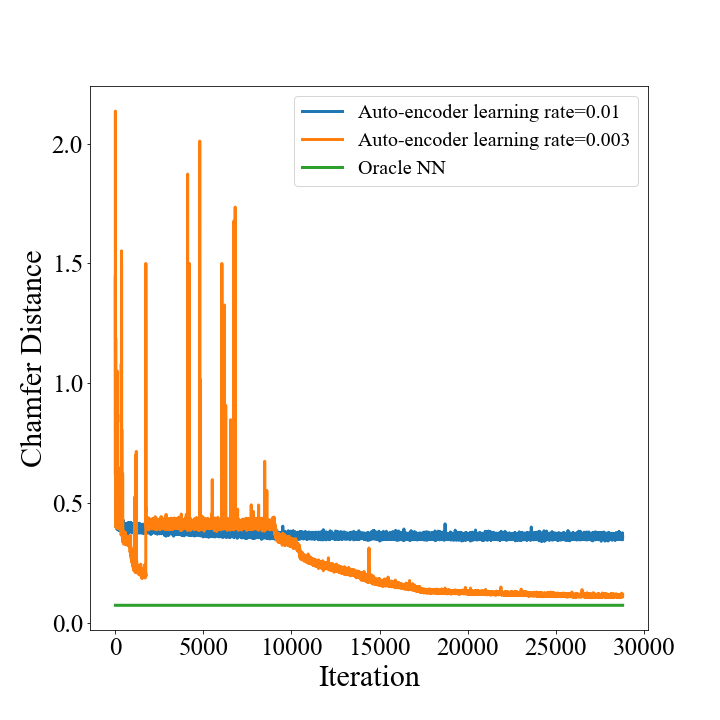
\includegraphics[width=\columnwidth]{figs/model/ae_trainingloss.png}
         \caption{训练集损失}\label{fig:trainingloss}
       \end{subfigure}
      \begin{subfigure}[t]{0.49\linewidth} \centering
          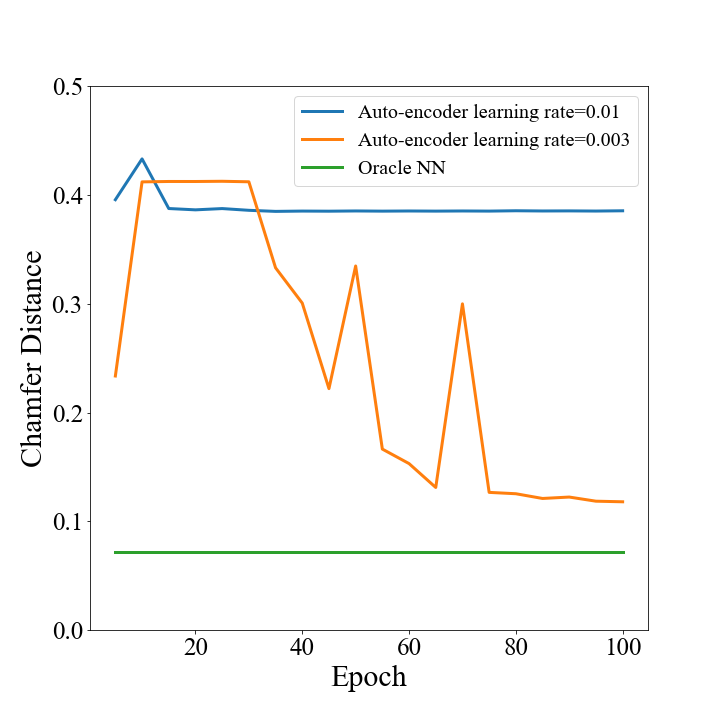
\includegraphics[width=\columnwidth]{figs//model/ae_testloss.png}
          \caption{测试集损失}\label{fig:testloss}
      \end{subfigure}
       \caption{\small 深度神经网络基准模型的两次训练过程。蓝色与橙色指同一网络在不同优化器学习率下的训练,绿色指非深度学习基准模型的量化结果}
    \label{fig:lossplot}
\end{figure}

\FloatBarrier
\section{模型优化}
\subsection{架构优化}\label{sec:optimal_method}
在这个部分,我们介绍用残差层改进解码器以及引入弱标签信息进行多任务训练这两种方法的实现细节以及使用这两种方法的原因。

\noindent
\textbf{引入弱标签信息进行多任务训练}

针对如何给网络参数提供良好的初始化,以及给编码器显性优化指导的问题,首先考虑图像深度学习领域常用的方法,即使用预训练的网络参数
进行网络初始化,具体来说,某任务需要使用神经网络进行图片分类前,会先把网络在ImageNet上训练到收敛后,再把网络在任务数据集上训练进行微调(fine-tuning),
我们没有采用这种预训练参数进行初始化的方法。一是因为ShapeNet的图片是由三维网格渲染而成的合成图片,ImageNet等图片分类数据集绝大部分图片来自现实世界图片,
这两个数据域的分布不同,因此需要考虑域适应的问题。二是如果在ShapeNet上预先训练图像分类网络,增加了三维重建的所需的步骤(变成了训练两个网络)和所需的计算资源。

基于上述的常用方法的启发,以及需要对编码器进行明显的训练指导的需求,我们提出加入弱标签信息进行多任务训练以达到初始化的目的。在训练的前5个周期,提供类标签给网络,在预测重建点云的同时将码字从中间层抽出进行图像分类训练,如图\ref{fig:class_init}。
在第6个周期以及之后取消这图片分类训练,只进行三维点云重建训练。关于多任务训练,我们原本有两个选择,一是图片分类,二是图片重建,增加这两种训练损失的任一种
从理论上来说都能指导编码器提取图片的某一种特征,比如分类任务会更关注于全局特征,而重建任务会关注局部特征,但是经过实验表明增加分类损失对三维重建
的效果提高比增加图片重建损失更加明显,所以我们选择加入分类任务来进行编码器初始化。

\begin{figure}
    \centering
    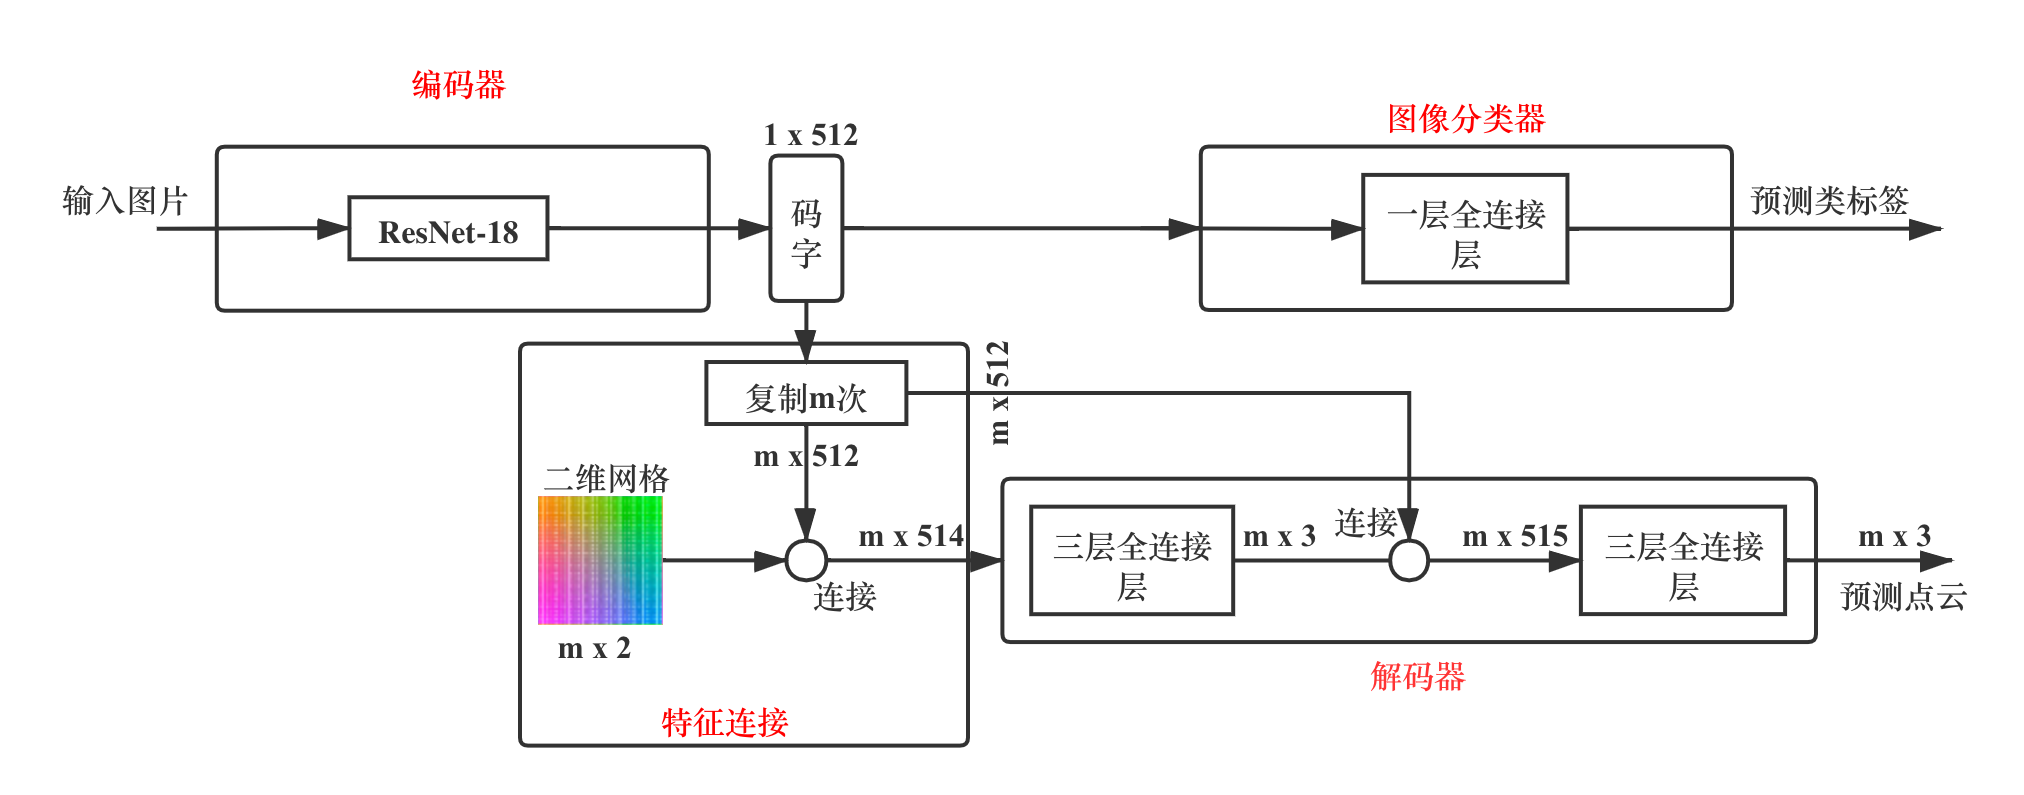
\includegraphics[width=0.99\columnwidth]{figs/model/ae_baseline_class.png}
    \caption{引入弱标签信息进行初始化}
    \label{fig:class_init}
\end{figure}
\FloatBarrier

\noindent
\textbf{使用残差层改进解码器结构}
\label{sec:resnet_decoder}

针对深度神经网络梯度消失的问题,一般的解决方法有:1)使用其他激活函数,如ReLU等;2)批归一化;3)优化网络权重的初始化方式,如xavier的参数初始化方法。4)调整网络结构,使用残差网络结构。

因为我们在基准模型中已经使用了ReLU作为激活函数,使用xavier初始化全连接层,所以我们主要使用第四种方法,即调整网络结构,辅助以批归一化。

具体的实现方法为用残差层改进基准模型\ref{fig:ae_baseline}的译码器,将三层全连接层感知器改为
由三个残差块组成的感知器,如图\ref{fig:resnet_decoder}。且残差块内部全连接层之间进行批处理归一化,改进后译码器的参数量是基准模型译码器的两倍,
保留译码器之前编码器和特征连接结构不变。残差层对于解码器的优化在于,通过引入“捷径连接”的方式,一方面在反向传播时,增大梯度的绝对值,另一方面改变了学习目标,
不再学习一个完整的输出,而是学习一个恒等映射,将网络部分的残差结果逼近于0,降低了网络学习的难度。批处理归一化通过
将每个隐层神经元的输入分布强制拉回到均值为0方差为1的标准正态分布,使得非线性变换函数的输入值落入对输入比较敏感的区域,
以此避免梯度消失的问题。


\begin{figure}
    \centering
    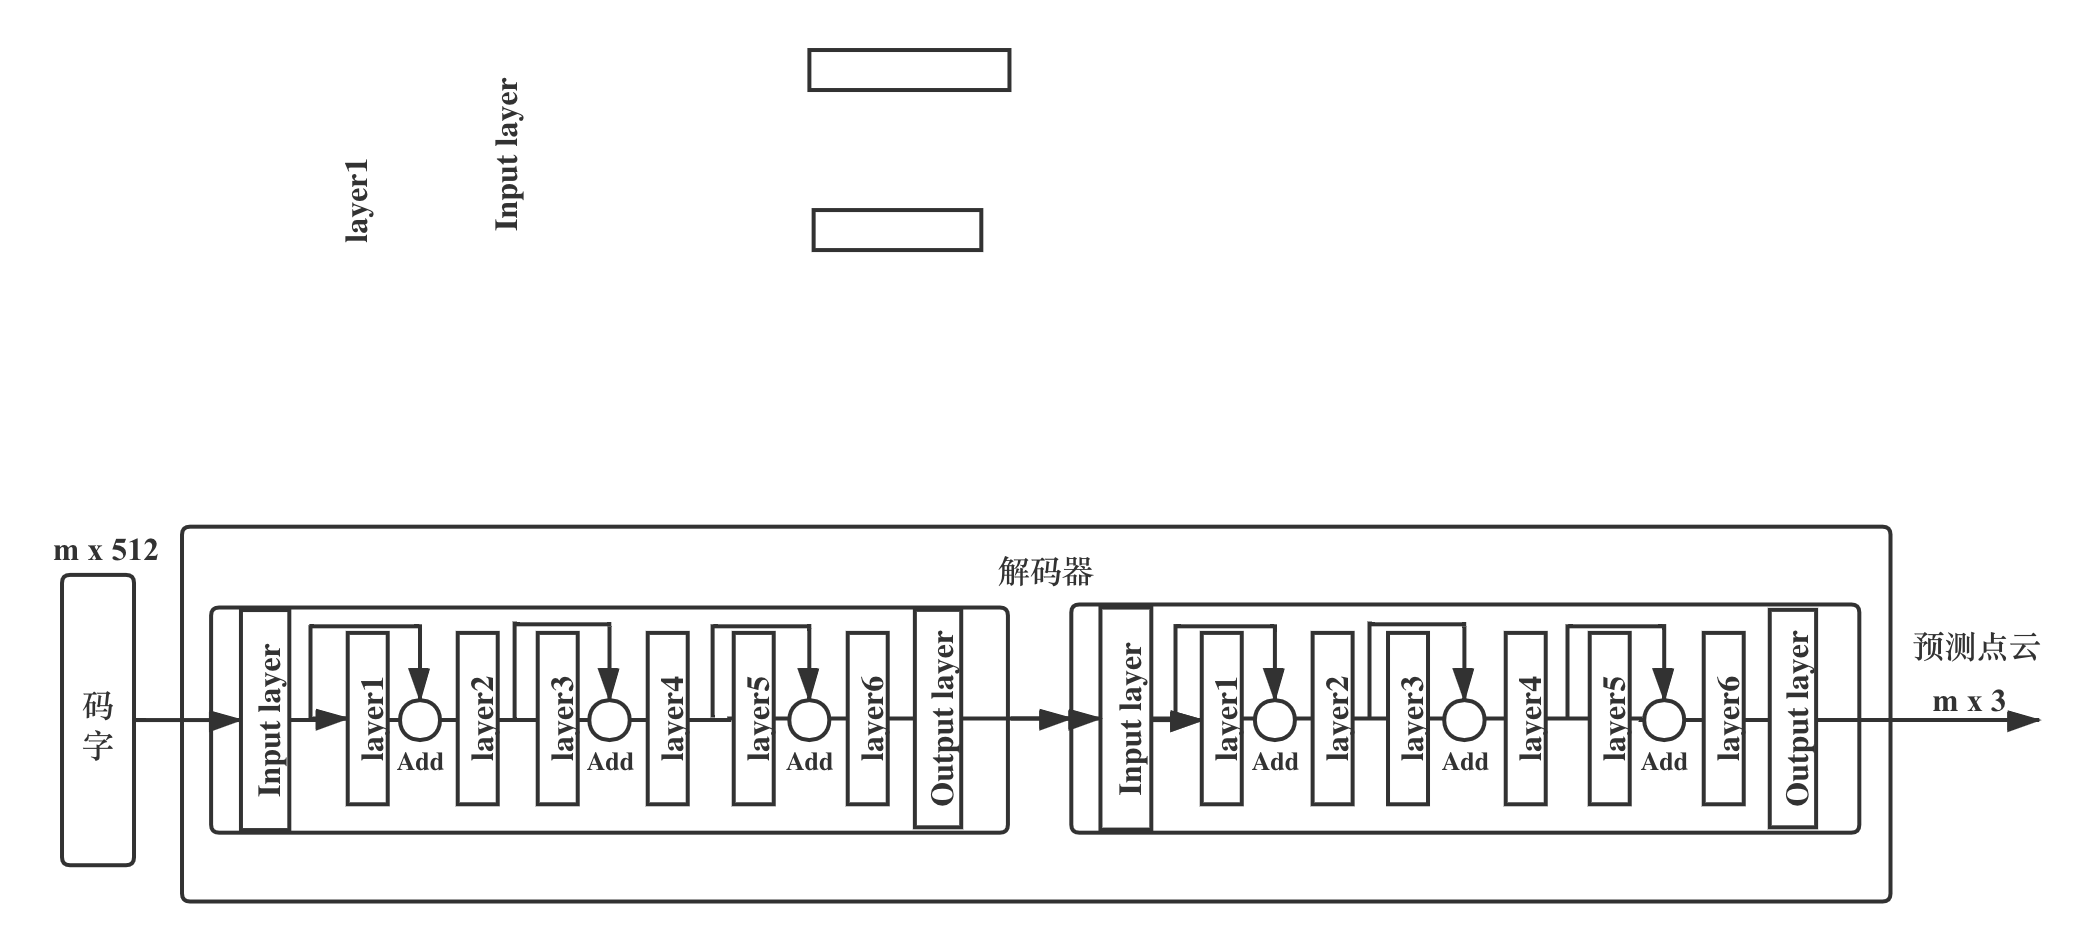
\includegraphics[width=0.99\columnwidth]{figs/model/resnet_decoder.png}
    \caption{用残差层改进译码器}
    \label{fig:resnet_decoder}
\end{figure}

\FloatBarrier



\subsection{实验结果与分析}
\label{sec:shapenet_result}
在这个部分,我们展示了将上述两种方法分别应用于优化网络,会在Chamfer Distance和F-score两个指标上取得接近甚至超过Oracle-NN的重建效果。
同时,我们进一步对深度神经网络的内在机制进行探究,展示了一个标准的三维重建深度神经网络在公开数据集ShapeNet上倾向于执行重建任务而不是识别任务。

\noindent
\textbf{重建效果}

表\ref{table:metric_optimal_baseline}汇报了基准模型,两种优化模型以及Oracle-NN的最优平均重建损失(Chamfer Distance),
数值越小说明重建效果越好,我们可以看到加入弱标签信息进行初始化后,基于自编码器的深度神经网络的重建水平(0.0716)优于Oracle-NN(0.0719),使用残差层解码器后,
神经网络的水平(0.0768)也得到了显著提高。特别的,我们将两个优化模型和Oracle-NN的Chamfer Distance表示在图\ref{fig:chamfer-compare},
从该图可以直观的看出,标准的基于自编码器的深度神经网络模型与Oracle-NN呈现出近乎相同的重建效果,且Oracle-NN(基于识别机制的非学习模型的理论极限)在测试时需要不应获得的标签信息。

除了Chamfer Distance这个指标外,我们还使用了F-score这个指标,将测试结果展现在\ref{fig:fscore-compare},这个指标下的模型比较结果与Chamfer Distance的比较
一致。因此,我们可以确定的得出结论:弱标签初始化与残差层改进都成功提高了深度神经网络在ShapeNet整体数据集的平均重建效果,
前者上超过了基于识别机制的非学习模型的理论极限,后者接近了这一理论极限。

\begin{table}
    \centering
    \caption{优化模型的评估结果}
    \begin{tabular}{ccc} 
    \hline
    模型                      & Chamfer Distance \\
    \hline
    自编码器(基准模型)            & 0.0806     \\
    自编码器(弱标签信息)           & 0.0716                             \\
    自编码器(残差层译码器)         & 0.0768                         \\
    Oracle-NN & 0.0719                           \\
    \hline
    \end{tabular}
    \label{table:metric_optimal_baseline}
\end{table}

\begin{figure}[!htb]
    \centering
    \begin{subfigure}[t]{0.49\linewidth} \centering 
        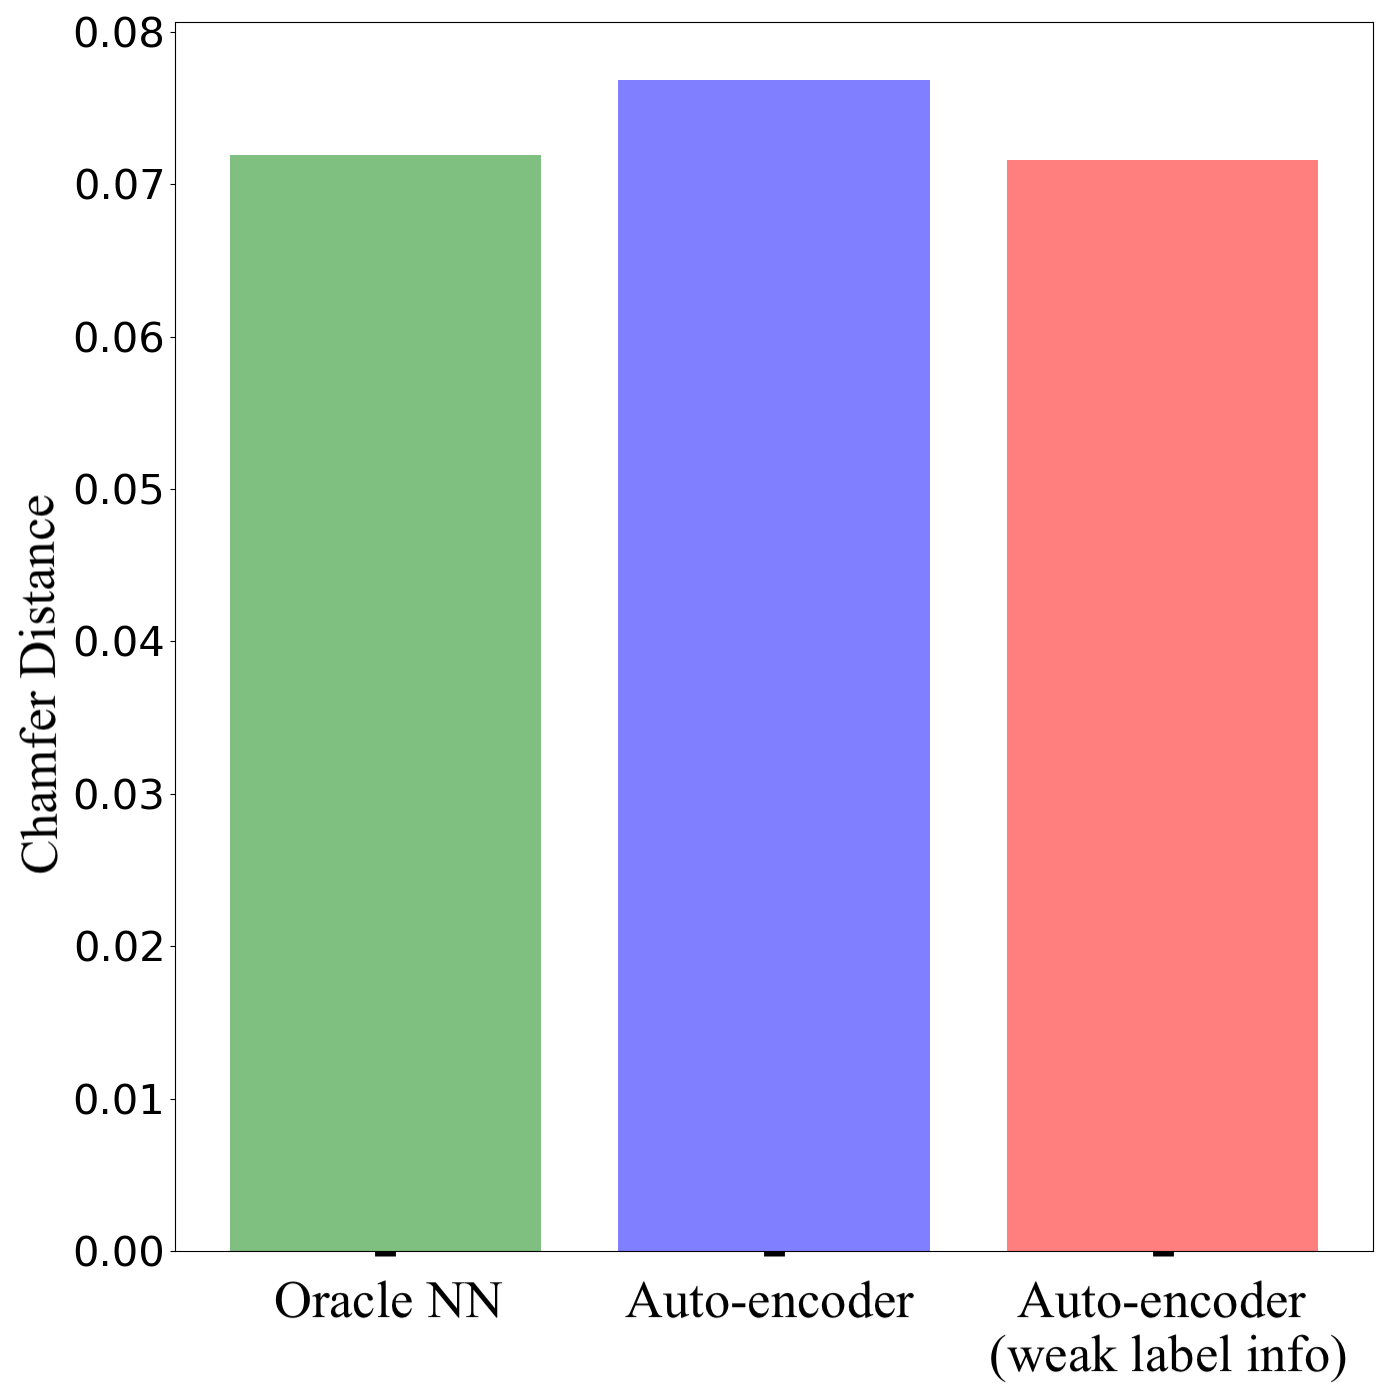
\includegraphics[width=\columnwidth]{figs/chamfer-compare_roman.png}
        \caption{各模型的Chamfer Distance比较}\label{fig:chamfer-compare}
      \end{subfigure}
     \begin{subfigure}[t]{0.49\linewidth} \centering
         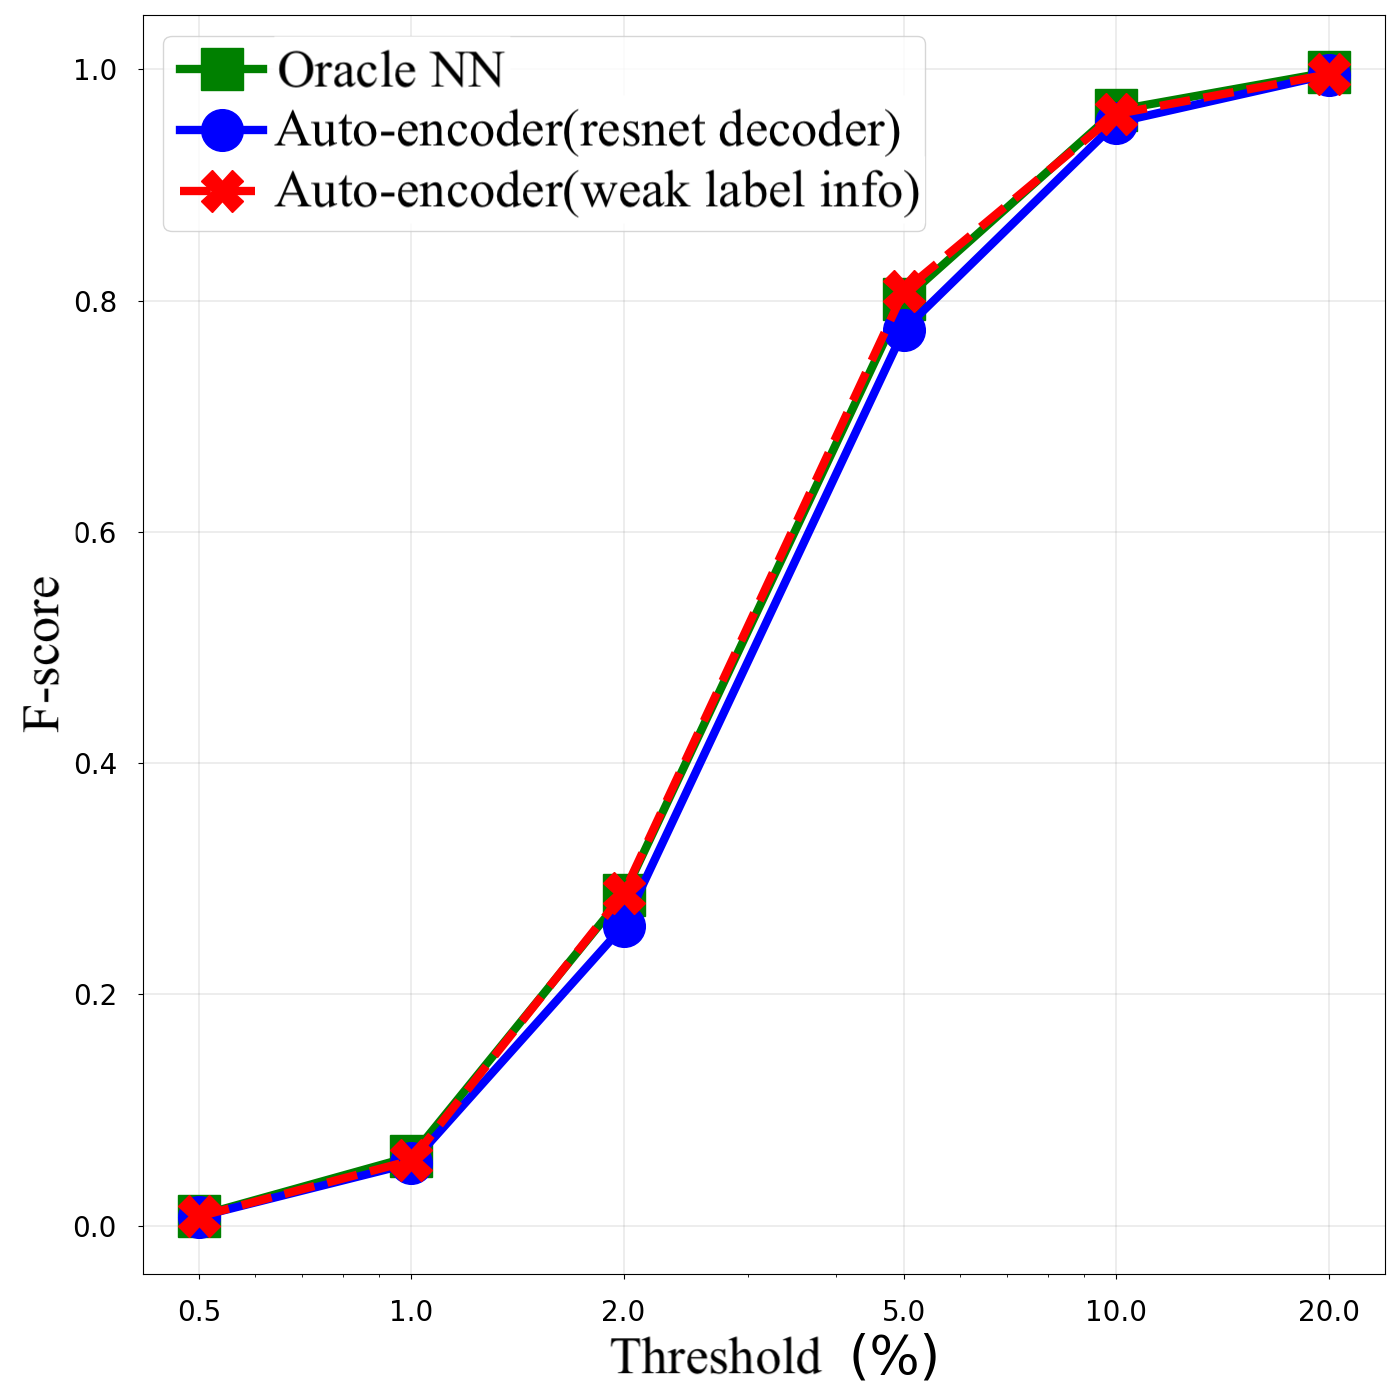
\includegraphics[width=\columnwidth]{figs/F-compare_roman.png}
         \caption{各模型的F-score比较}\label{fig:fscore-compare}
     \end{subfigure}
    \caption{\small 优化深度学习模型与非深度学习模型各指标比较}
    \label{fig:compare-Oracle-NN}
\end{figure}

除了平均重建效果,我们还考虑了每个类的重建结果的统计特性,如图\ref{fig:metric_per_class}。我们可以看到基于自编码器的三维重建神经网络在不同的类的
重建效果上下波动较小,近似一致。而Oracle-NN在一些类别如tower,呈现出非常差的重建效果,出现了各个类重建效果不一致的情况。这个问题同样也在模型预测结果可视化中呈现出来,如图
\ref{fig:visualize_KC}第四行,我们可以看到Oracle-NN预测出了在三维形状层面上非常不合理的点云。结合附录\ref{fig:data-stats}展示的ShapeNet数据集的分布,我们可以看到有一些类的样本量很少,
Oracle-NN在样本量少的类内进行搜索时,有很大概率无法找到与预测点云相近的训练点云,因此会在这些类出现比较差的重建效果。

图\ref{fig:visualize_KC}展示了各个模型预测结果的可视化,从这些定性结果可以看出,在不同物体类别之间,标准自动编码器的重建性能比Oracle-NN更稳定。
更多的可视化结果提供在附录\ref{fig:visualize_KC_supplementary}中。

综上所述,我们可以看出基于识别机制的非深度学习模型的局限性,此类模型缺少对训练数据集分布的鲁棒性,当训练集无法在低维度层面解释测试集需要的形状特征时(即当训练集中没有和测试样本在损失距离上相近的点云时),
该类模型的方法效果远差于深度学习模型。

\begin{figure}
\centering
\begin{tabular}{c@{}}
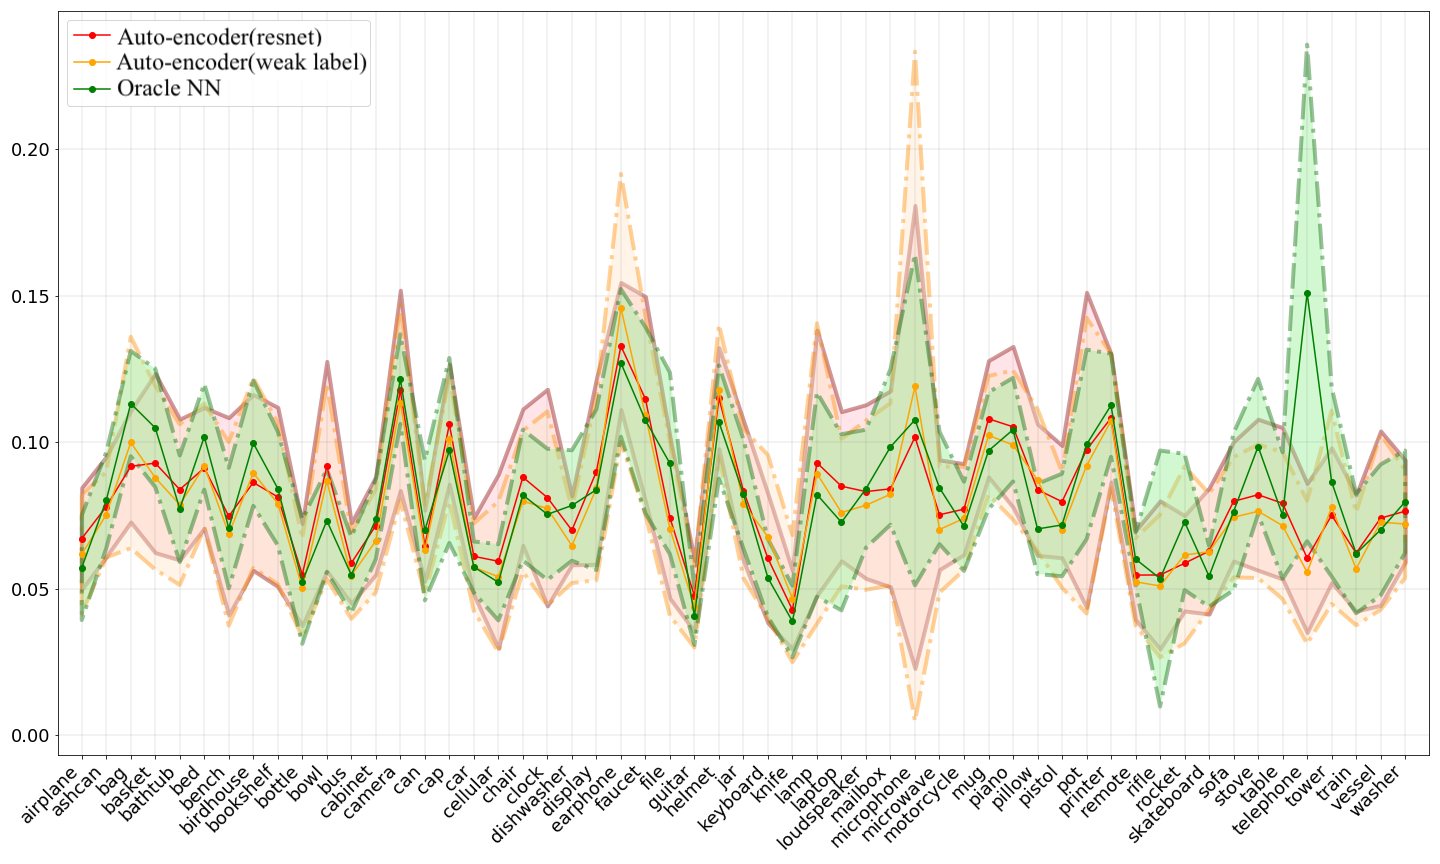
\includegraphics[width=0.99\columnwidth]{figs/CD_per_shape_roman.png} \\
Chamfer Distance \\
\end{tabular}
\caption{每个类的重建评价指标,X轴每一列代表一个类的Chamfer Distance统计。实心点代表类内所有样本指标平均值,
上边沿虚线代表类内所有样本指标最大值,下边沿虚线代表类内所有样本指标最小值。}
\label{fig:metric_per_class}
\end{figure}

\begin{figure}[!h]
    \begin{tabular}{c@{}c@{}c@{}c@{}c@{}}
    输入图片 & 标签点云 & \makecell[c]{自编码器 \\(弱标签信息)} & \makecell[c]{自编码器 \\(残差层译码器)} & Oracle-NN\\
    	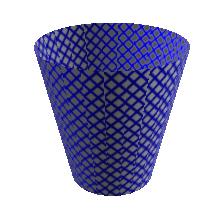
\includegraphics[width=0.11\columnwidth,height=2cm]{figs/real_dataset/Image/ashcan_ff2f13bc0b9d4ade19c52ba9902b5ab0.png} &
    	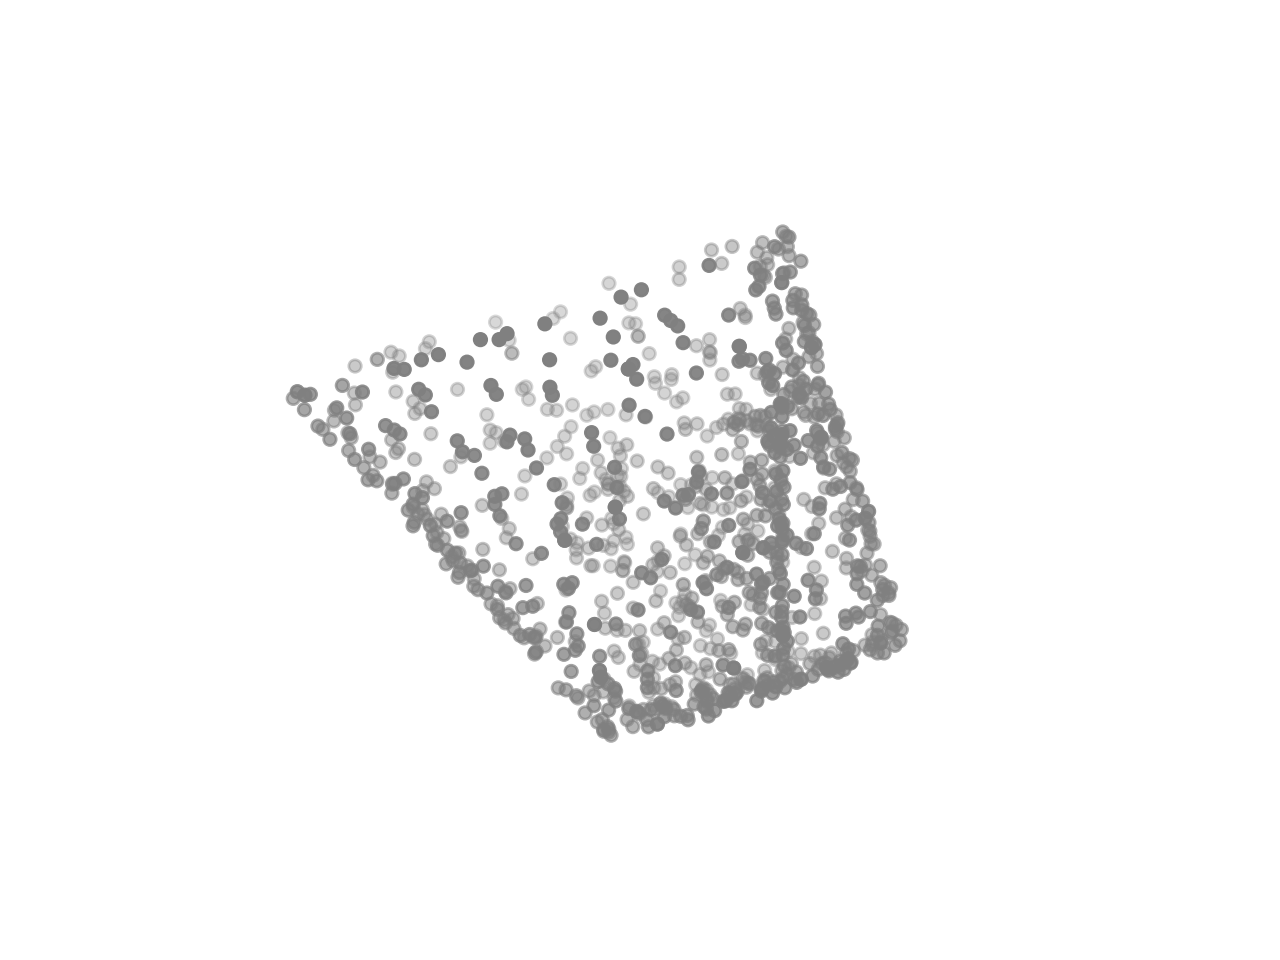
\includegraphics[width=0.22\columnwidth,height=2cm]{figs/real_dataset/GT/ashcan_ff2f13bc0b9d4ade19c52ba9902b5ab0_gt.png} &
    	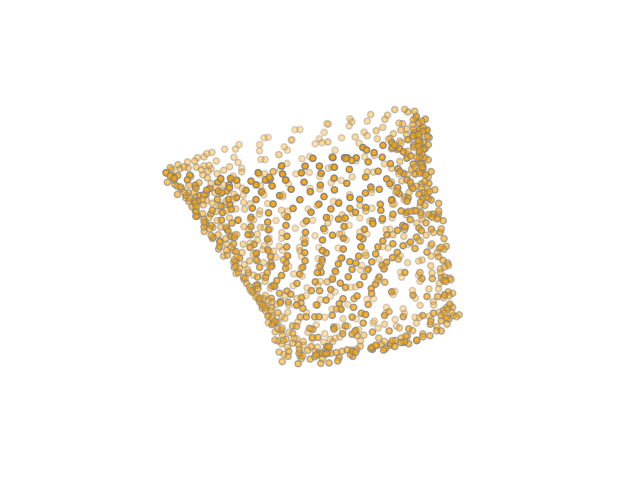
\includegraphics[width=0.22\columnwidth,height=2cm]{figs/real_dataset/AE_label/ashcan_ff2f13bc0b9d4ade19c52ba9902b5ab0_fine.png} &
    	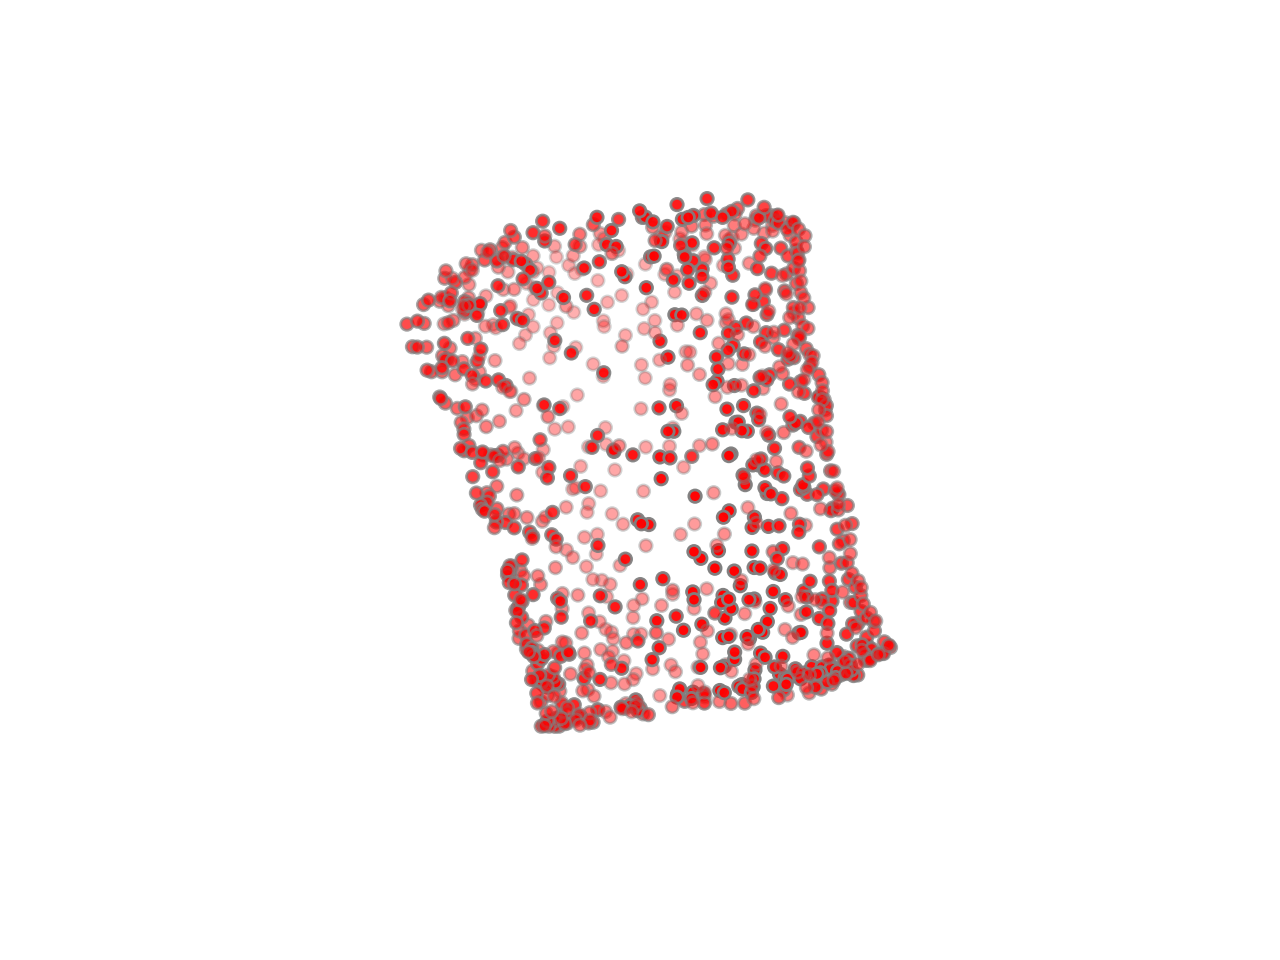
\includegraphics[width=0.22\columnwidth,height=2cm]{figs/real_dataset/AE/ashcan_66d96d2428184442ba6cf6cbb9f4c2bb_fine.png} &
    	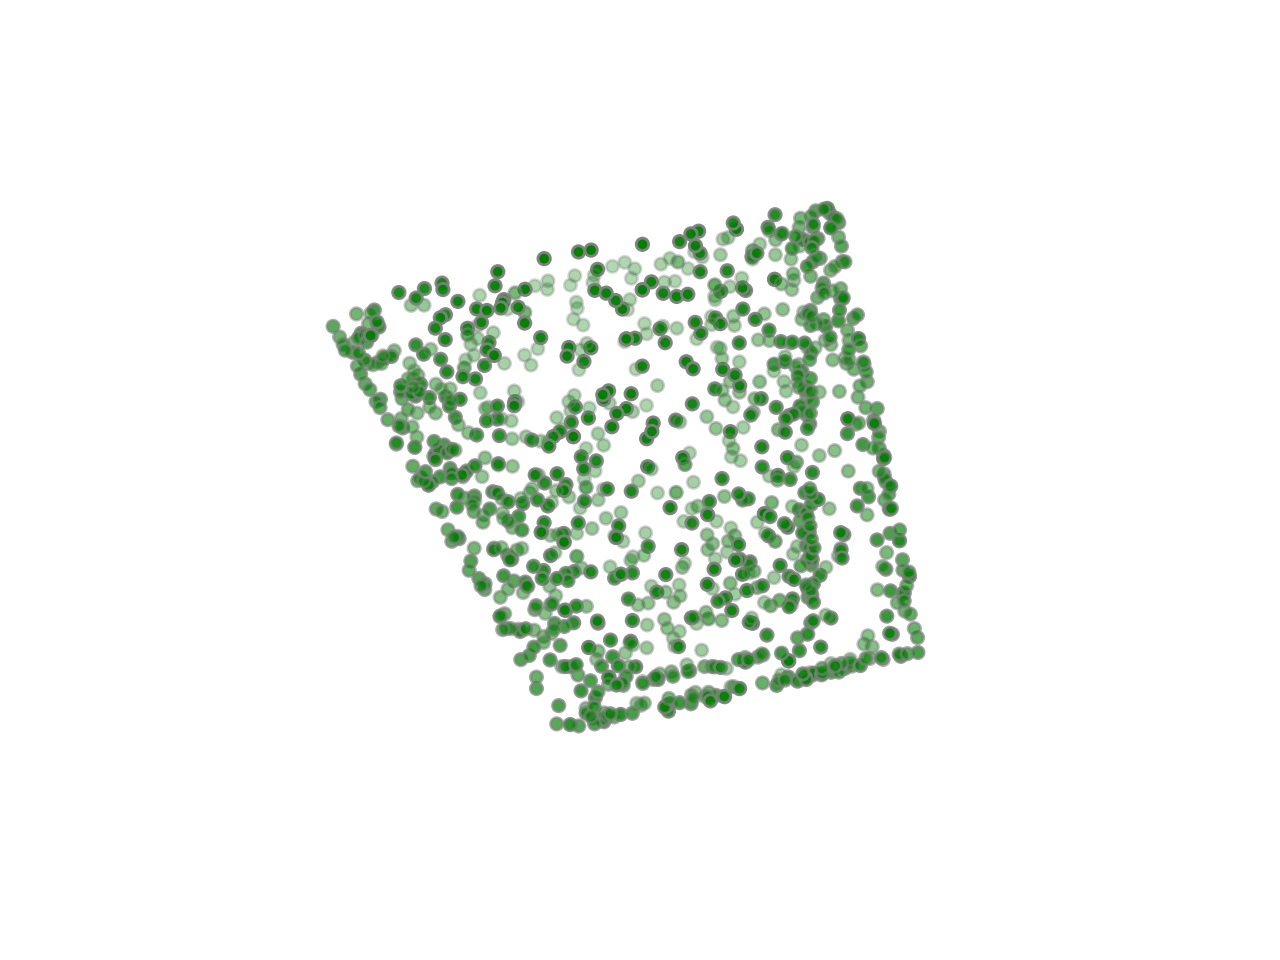
\includegraphics[width=0.22\columnwidth,height=2cm]{figs/real_dataset/oracle/ashcan_ff2f13bc0b9d4ade19c52ba9902b5ab0_oracle.png} \\
    	\vspace{-5mm}
    	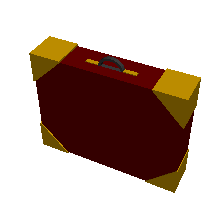
\includegraphics[width=0.11\columnwidth,height=2cm]{figs/real_dataset/Image/bag_8569a0c606bbba73d9985ad45fbb635e.png} &
    	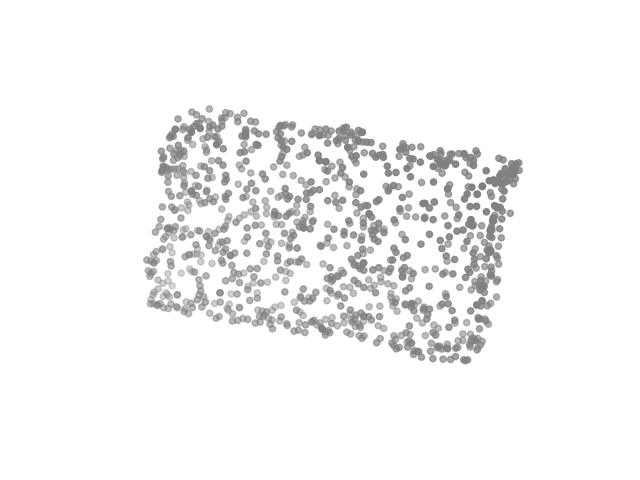
\includegraphics[width=0.22\columnwidth,height=2cm]{figs/real_dataset/GT/bag_8569a0c606bbba73d9985ad45fbb635e.png} &
    	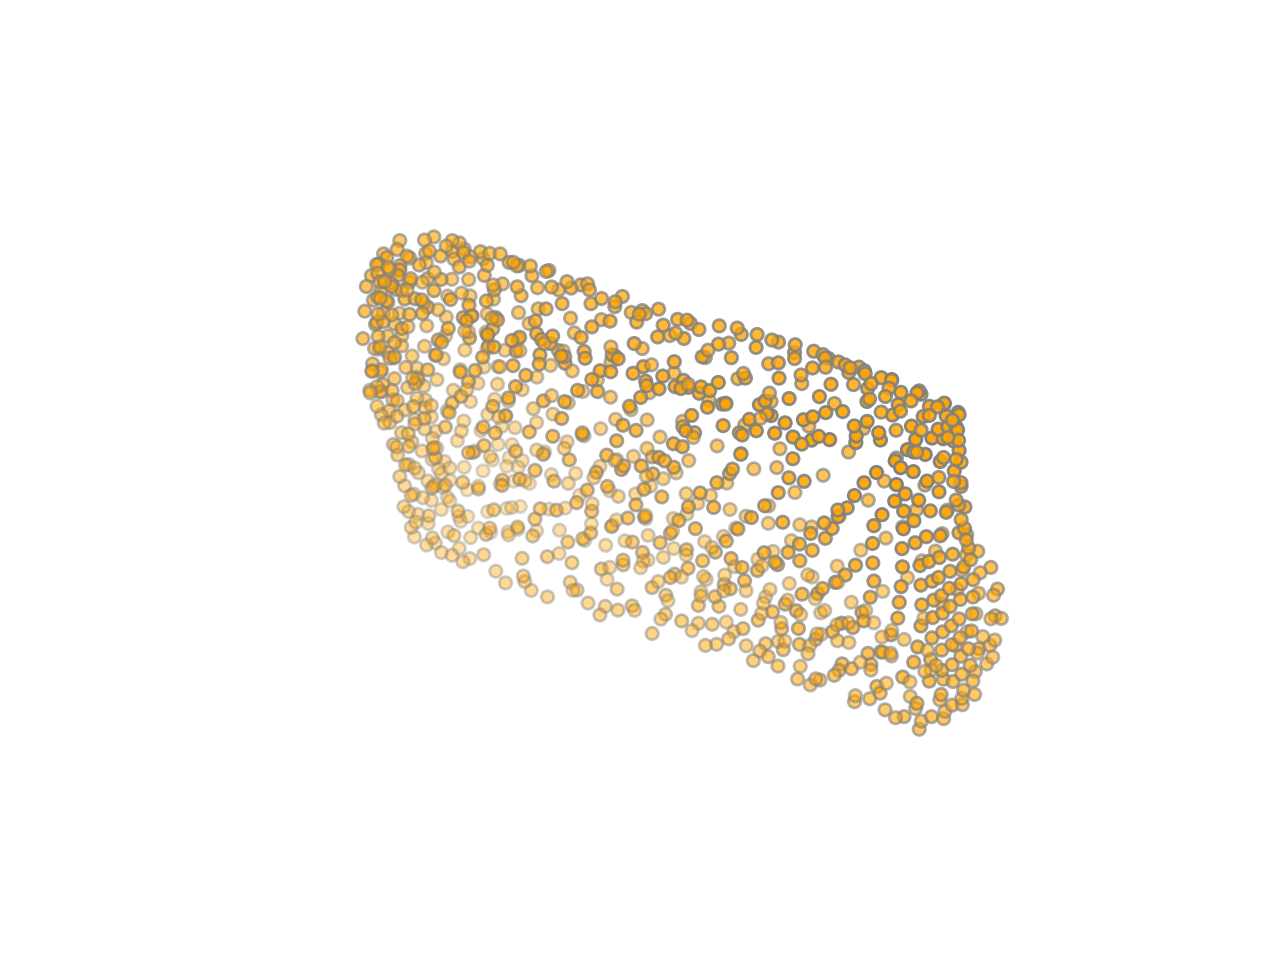
\includegraphics[width=0.22\columnwidth,height=2cm]{figs/real_dataset/AE_label/bag_8569a0c606bbba73d9985ad45fbb635e_fine.png} &
    	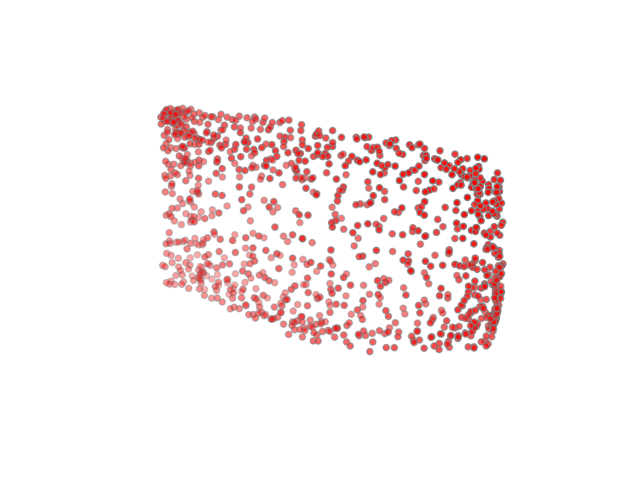
\includegraphics[width=0.22\columnwidth,height=2cm]{figs/real_dataset/AE/bag_8569a0c606bbba73d9985ad45fbb635e.png} &
    	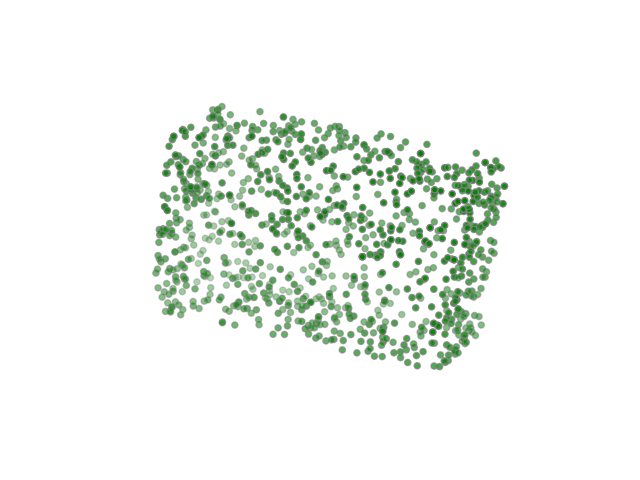
\includegraphics[width=0.22\columnwidth,height=2cm]{figs/real_dataset/oracle/bag_8569a0c606bbba73d9985ad45fbb635e.png} \\  
    	\vspace{-5mm}
    	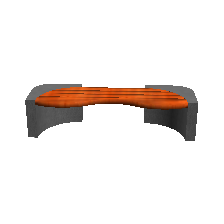
\includegraphics[width=0.11\columnwidth,height=2cm]{figs/real_dataset/Image/bench_17ebf60b6ba61ae949e6f7df978f3373.png} &
    	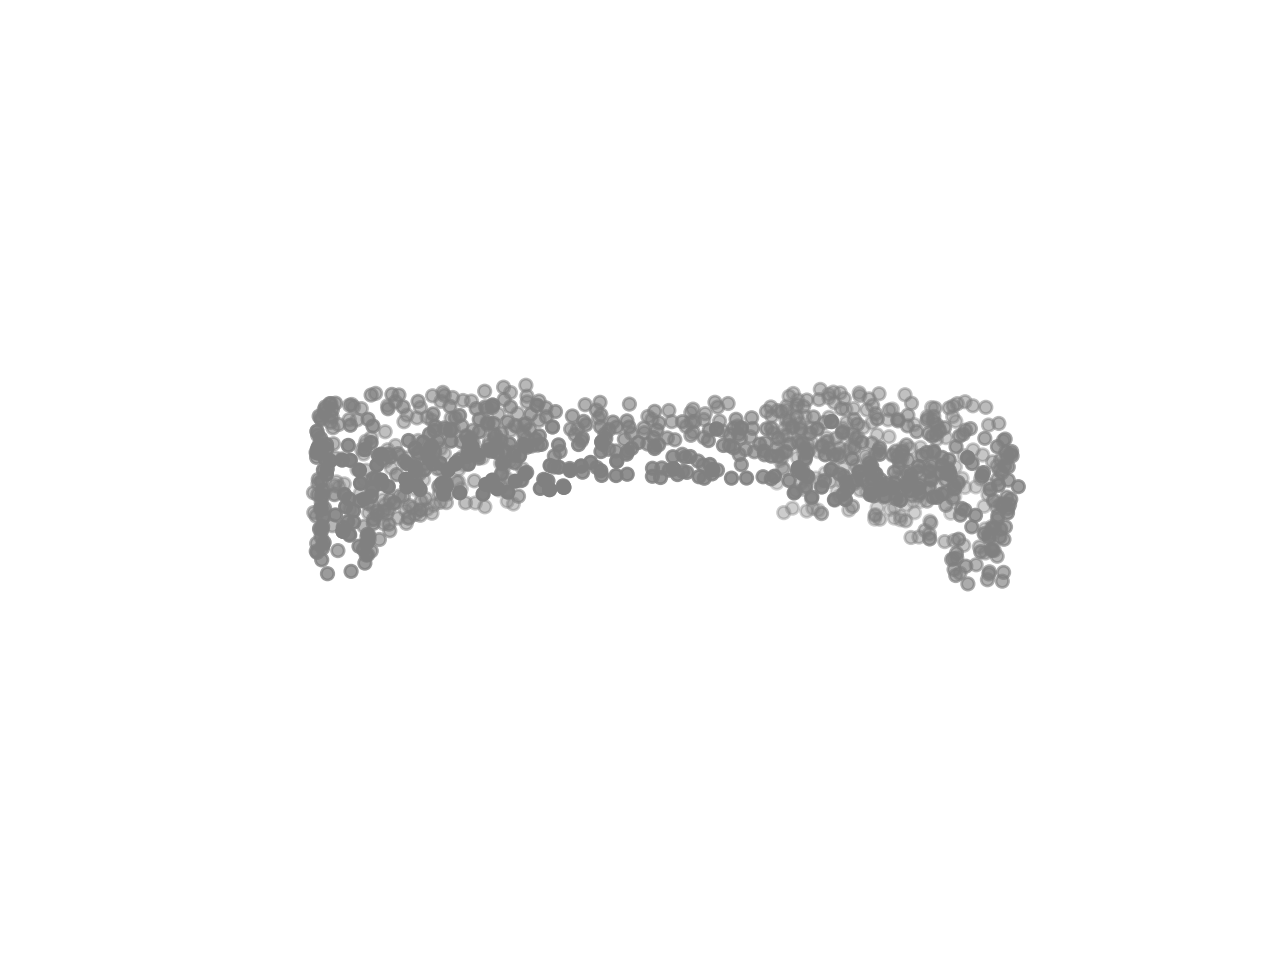
\includegraphics[width=0.22\columnwidth,height=2cm]{figs/real_dataset/GT/bench_17ebf60b6ba61ae949e6f7df978f3373_gt.png} &
    	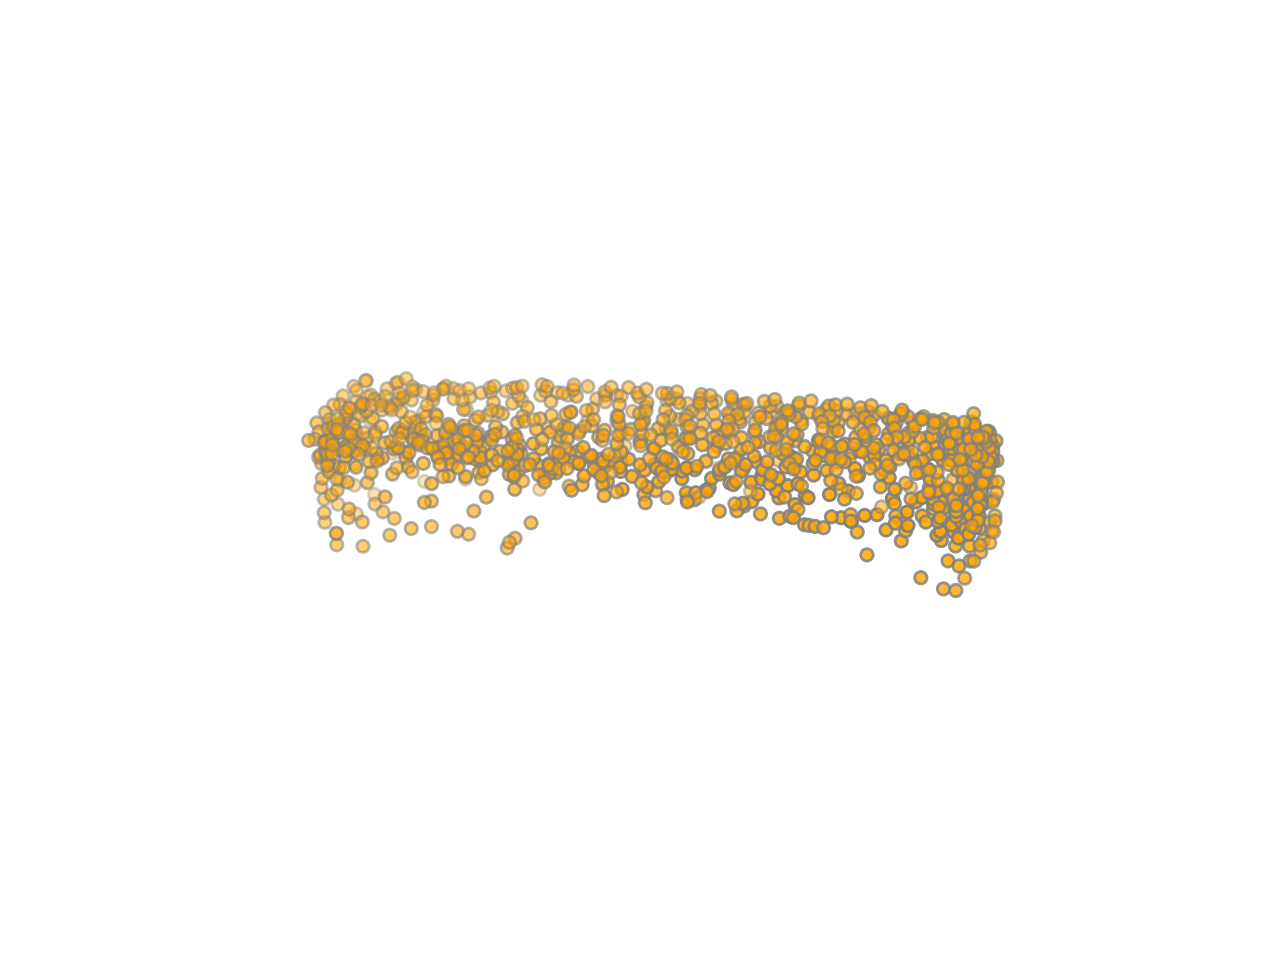
\includegraphics[width=0.22\columnwidth,height=2cm]{figs/real_dataset/AE_label/bench_17ebf60b6ba61ae949e6f7df978f3373_fine.png} &
    	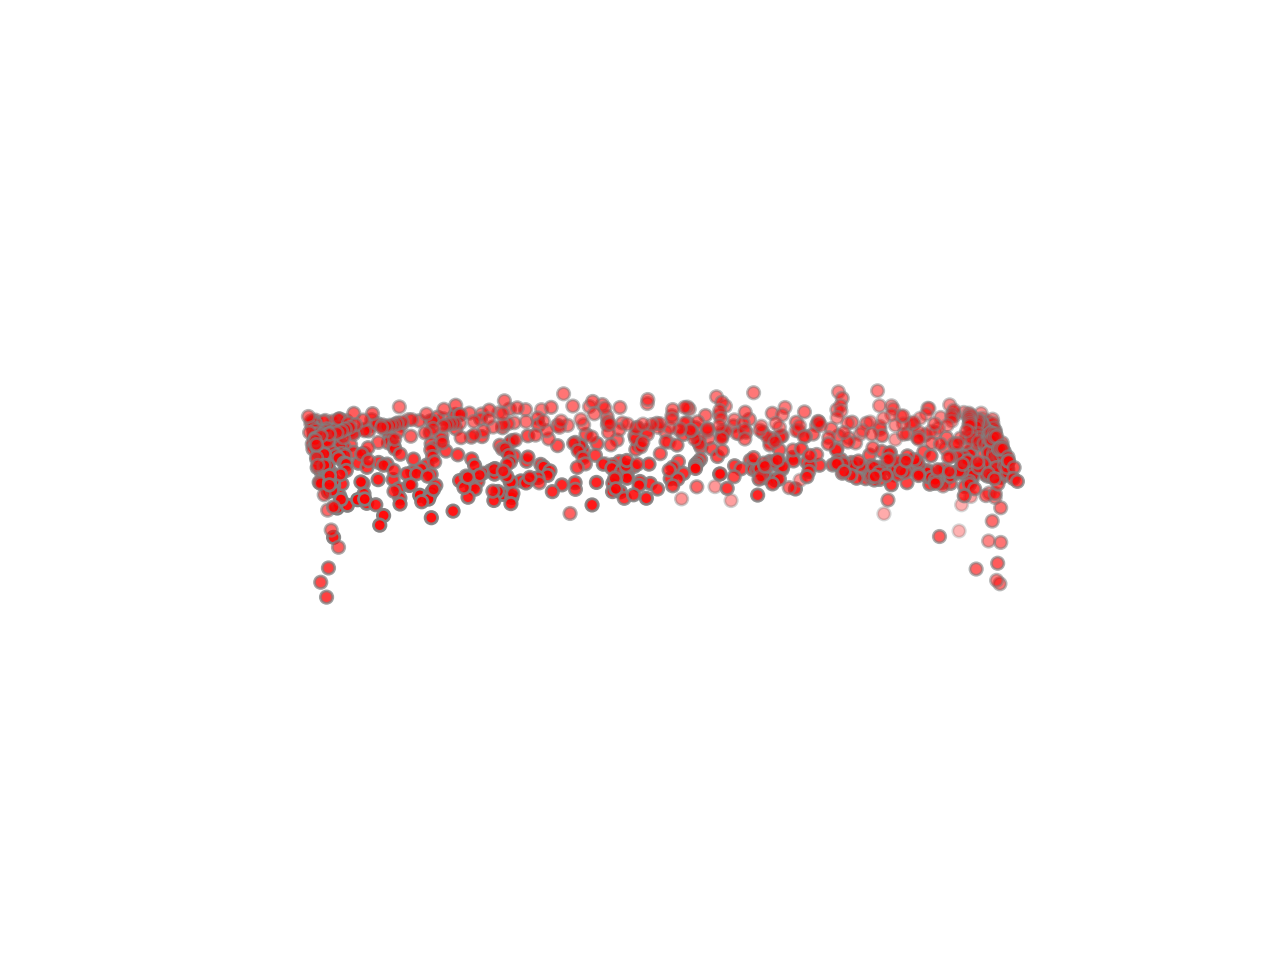
\includegraphics[width=0.22\columnwidth,height=2cm]{figs/real_dataset/AE/bench_17ebf60b6ba61ae949e6f7df978f3373_fine.png} &
    	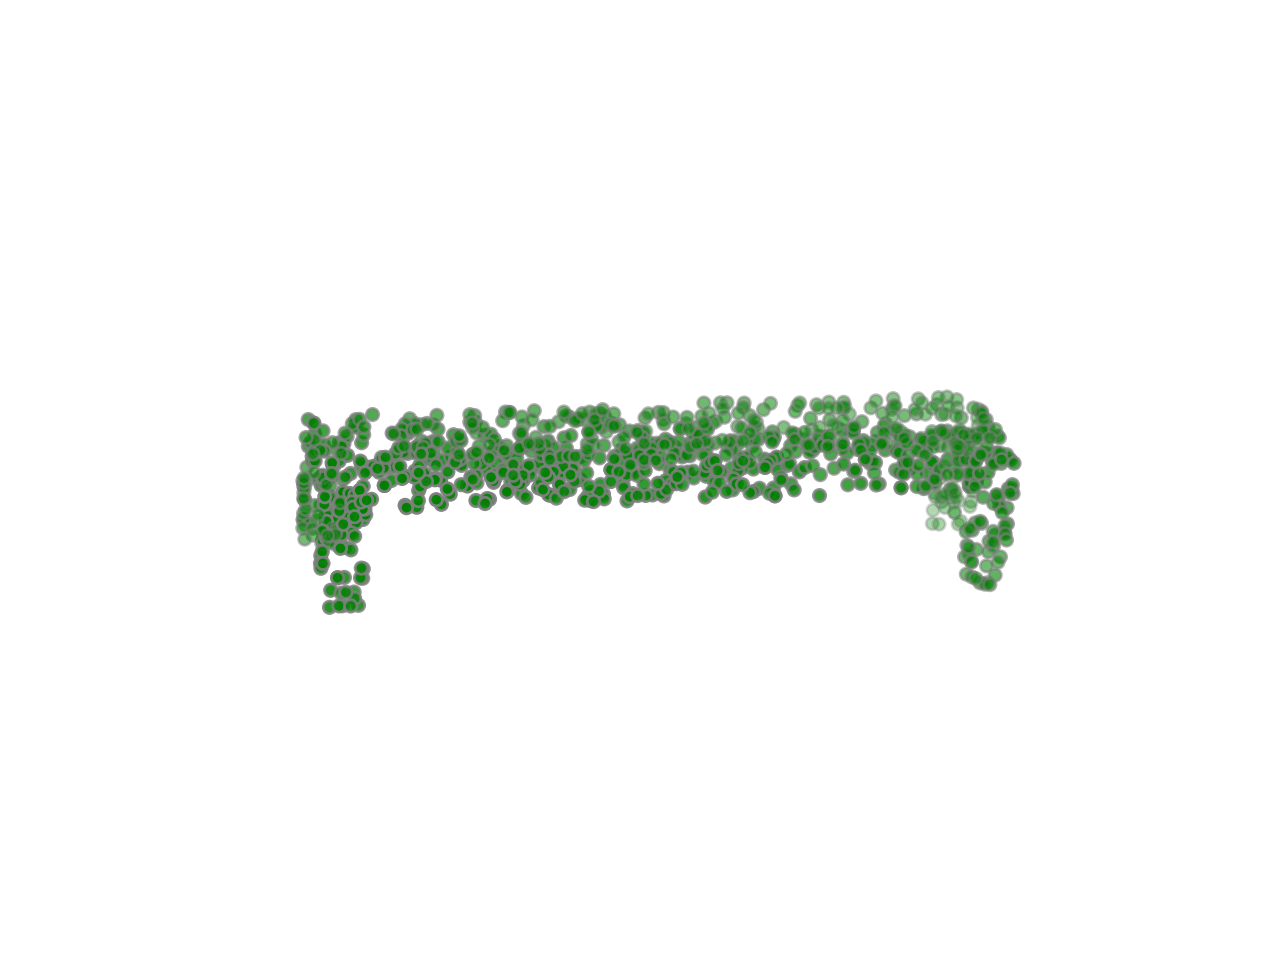
\includegraphics[width=0.22\columnwidth,height=2cm]{figs/real_dataset/oracle/bench_17ebf60b6ba61ae949e6f7df978f3373_oracle.png} \\
    	\vspace{-5mm}
    	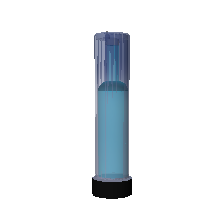
\includegraphics[width=0.11\columnwidth,height=2cm]{figs/real_dataset/Image/bottle_ab3795042c759b6798646029ad91cbbd.png} &
    	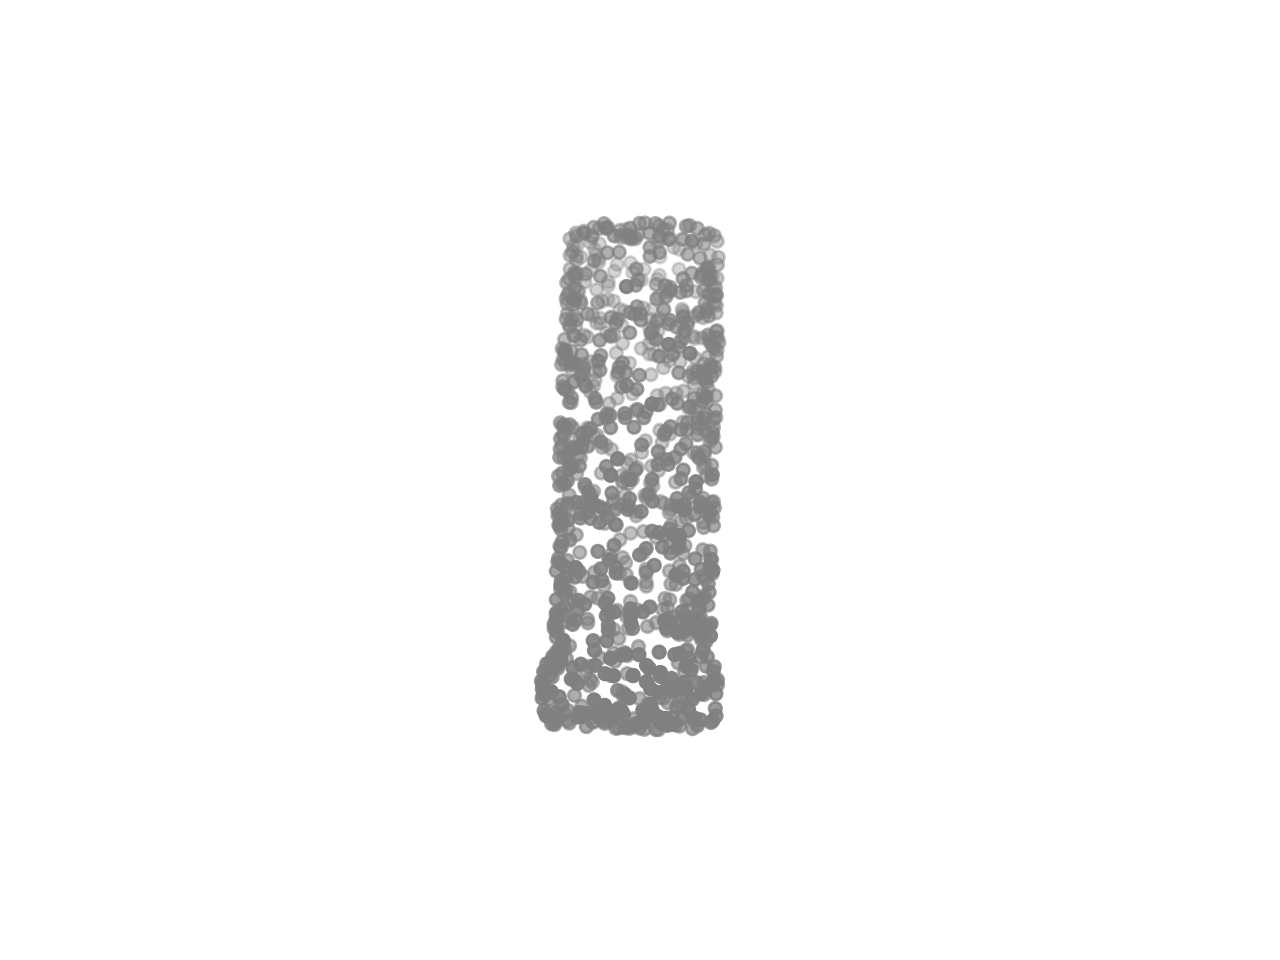
\includegraphics[width=0.22\columnwidth,height=2cm]{figs/real_dataset/GT/bottle_ab3795042c759b6798646029ad91cbbd_gt.png} &
    	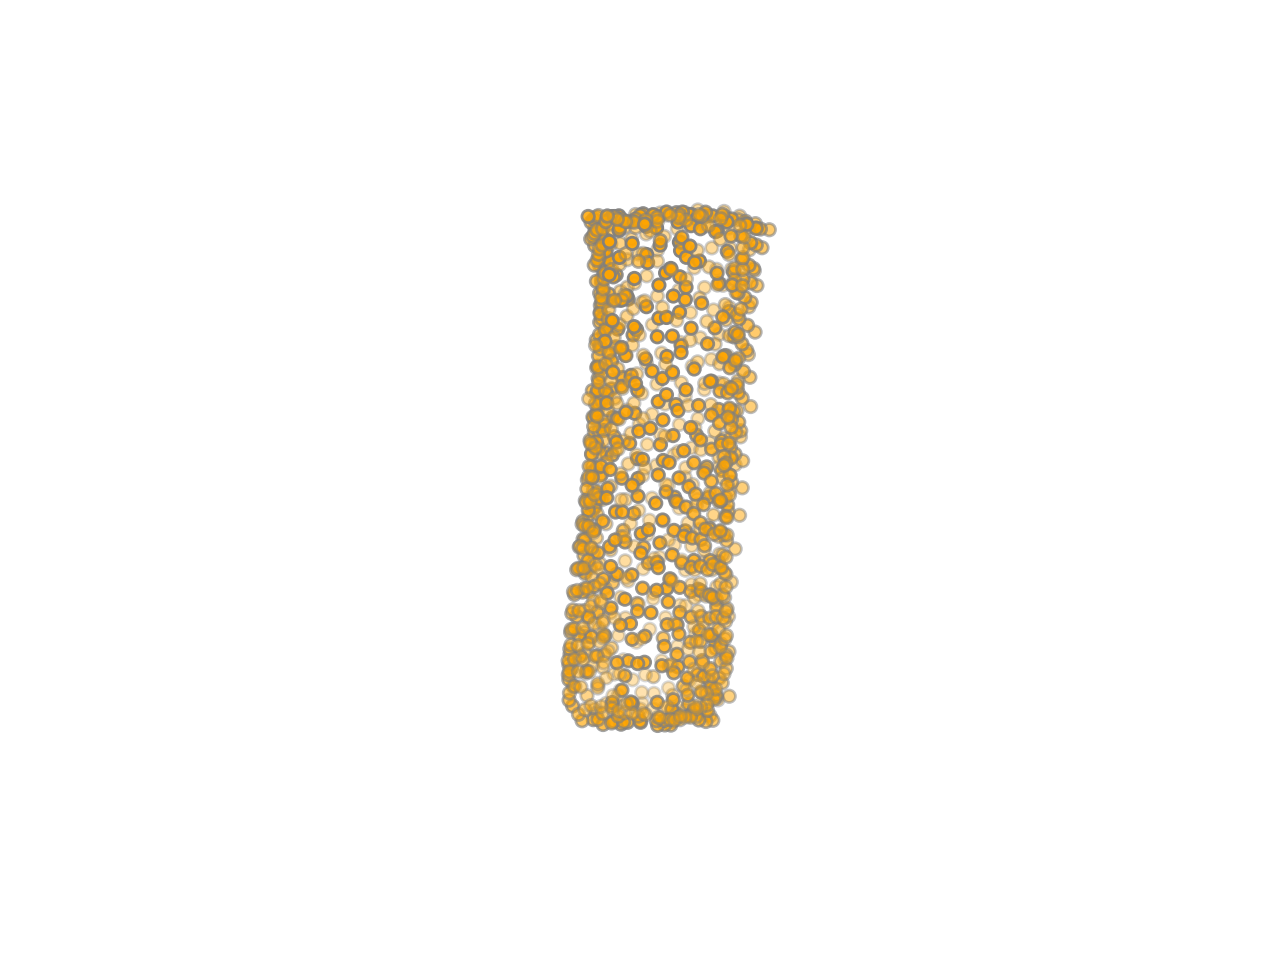
\includegraphics[width=0.22\columnwidth,height=2cm]{figs/real_dataset/AE_label/bottle_ab3795042c759b6798646029ad91cbbd_fine.png} &
    	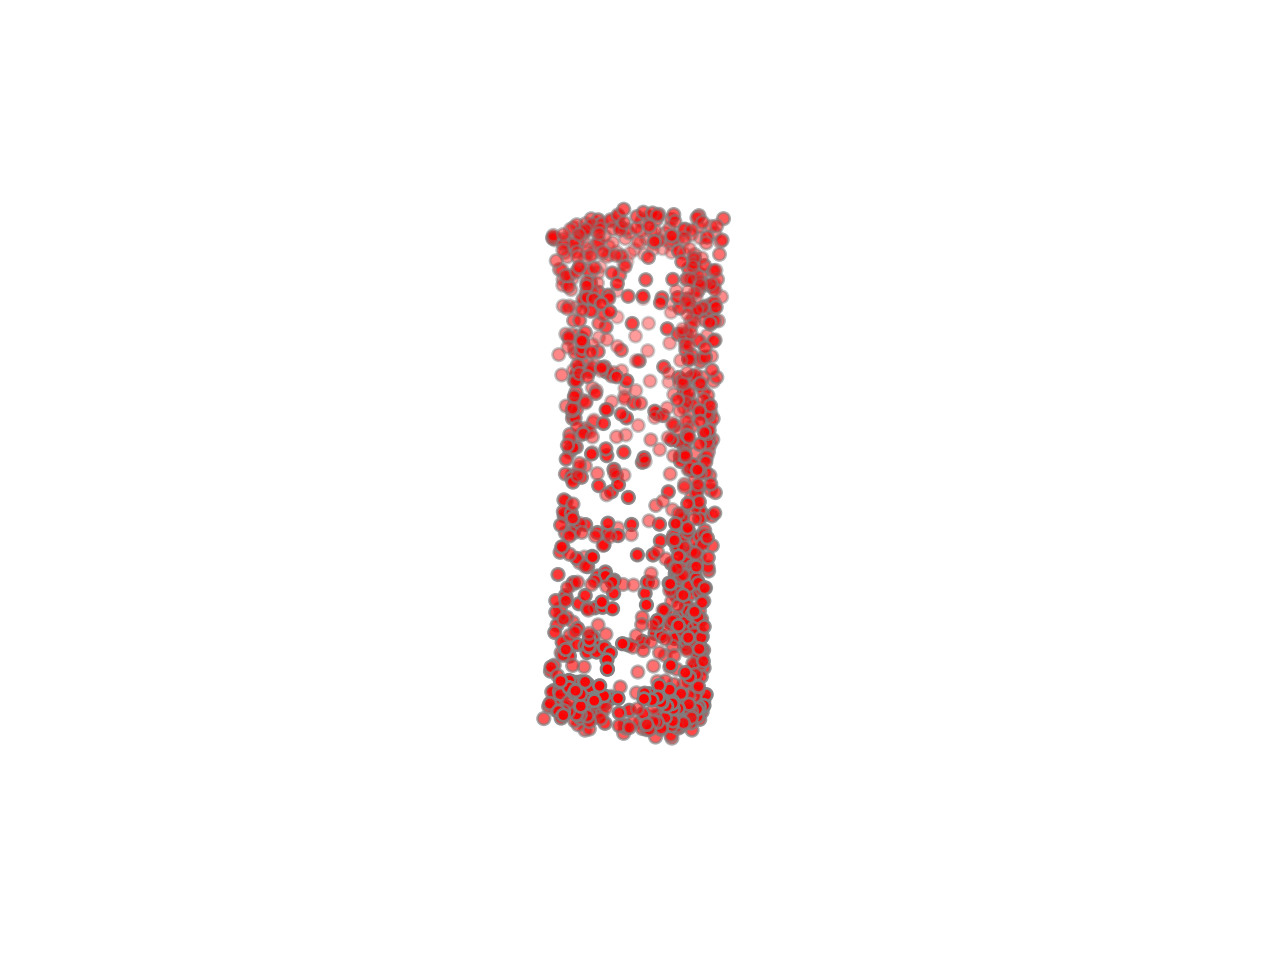
\includegraphics[width=0.22\columnwidth,height=2cm]{figs/real_dataset/AE/bottle_ab3795042c759b6798646029ad91cbbd_fine.png} &
    	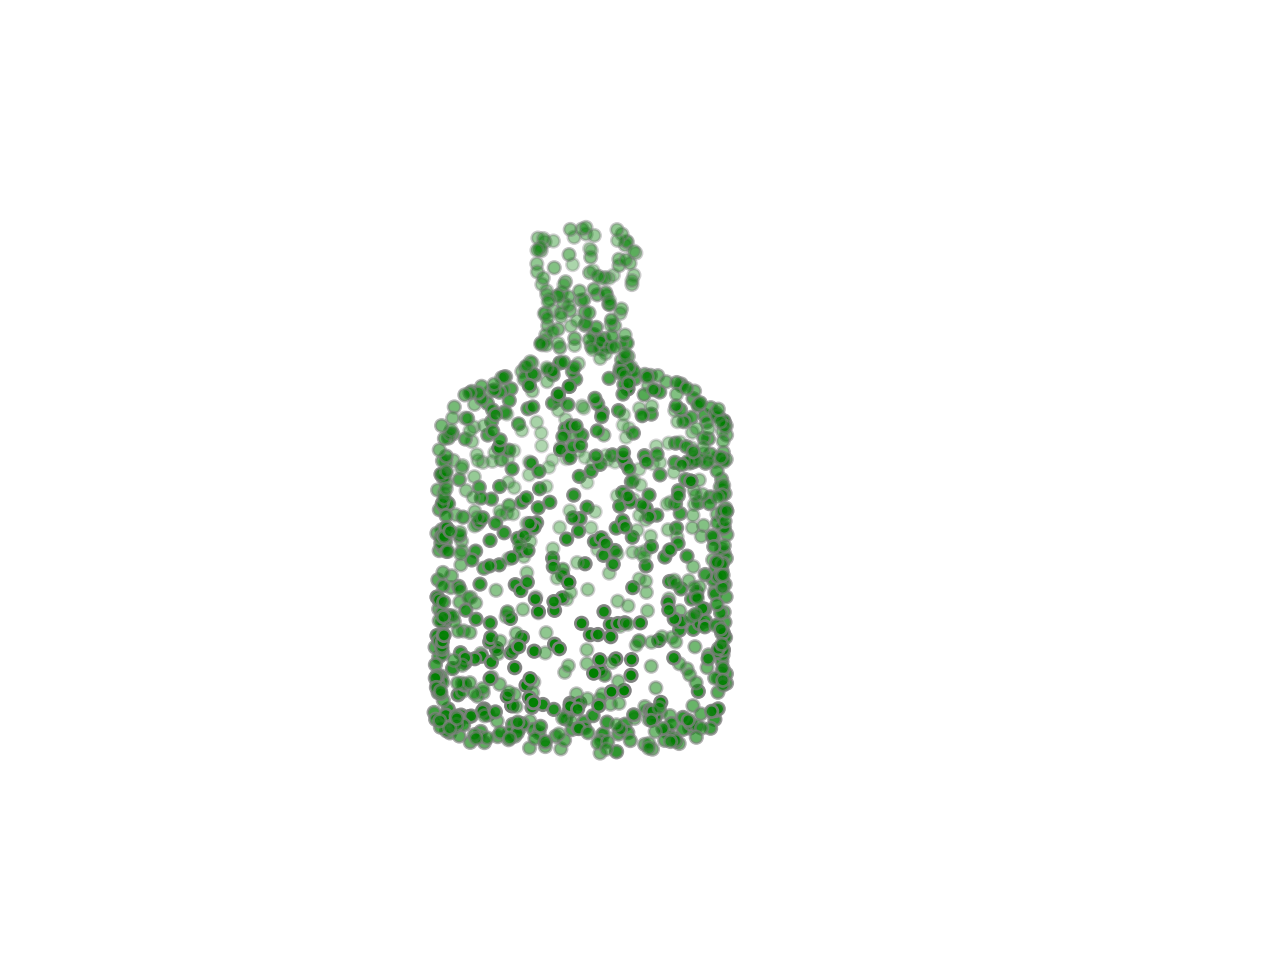
\includegraphics[width=0.22\columnwidth,height=2cm]{figs/real_dataset/oracle/bottle_3b956918a41da89c325e6e8eb2c67fd8_oracle.png} \\
    	\vspace{-5mm}
    	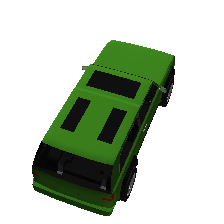
\includegraphics[width=0.11\columnwidth,height=2cm]{figs/real_dataset/Image/car_8b049c92888475f67c3c6f82a395b347.png} &
    	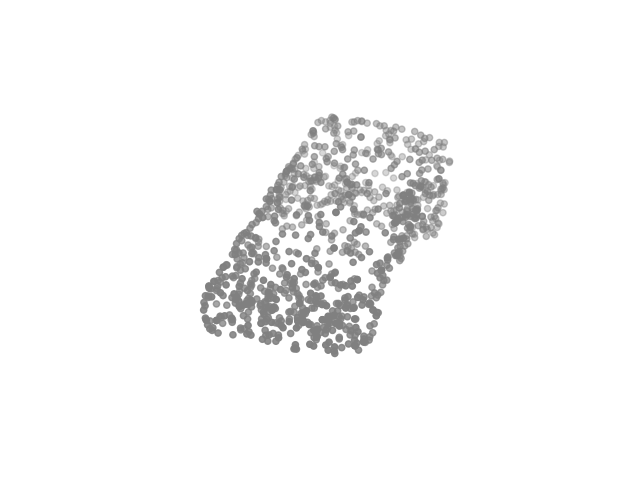
\includegraphics[width=0.22\columnwidth,height=2cm]{figs/real_dataset/GT/car_8b049c92888475f67c3c6f82a395b347.png} &
    	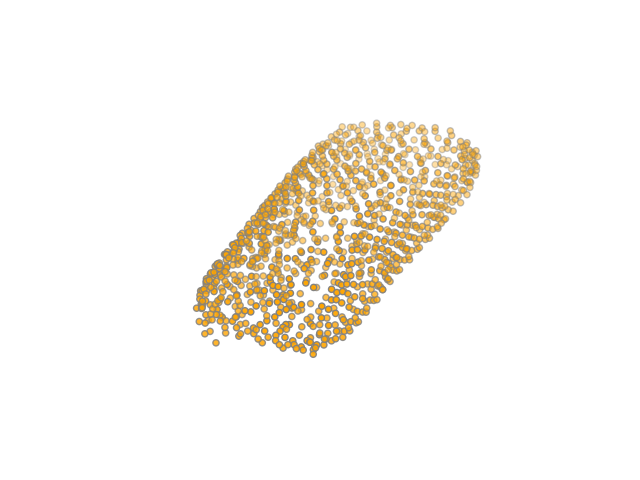
\includegraphics[width=0.22\columnwidth,height=2cm]{figs/real_dataset/AE_label/car_8b049c92888475f67c3c6f82a395b347_fine.png} &
    	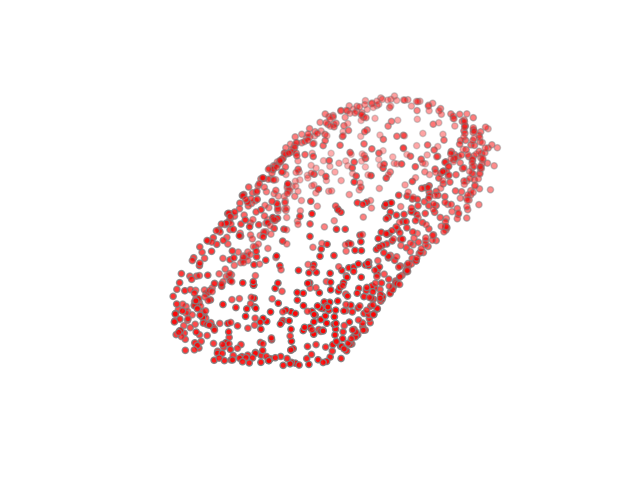
\includegraphics[width=0.22\columnwidth,height=2cm]{figs/real_dataset/AE/car_8b049c92888475f67c3c6f82a395b347.png} &
    	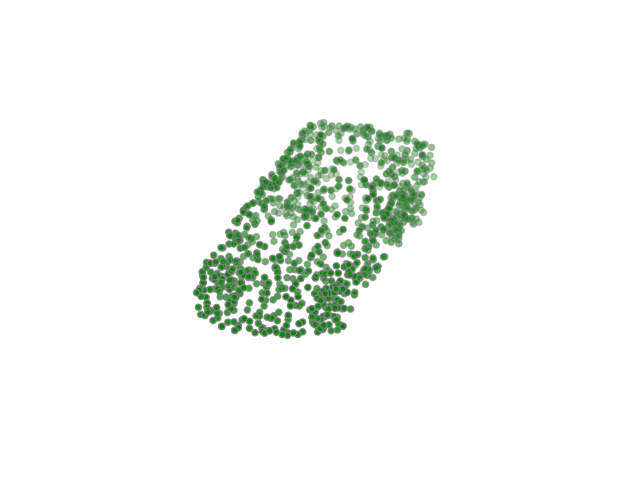
\includegraphics[width=0.22\columnwidth,height=2cm]{figs/real_dataset/oracle/car_8b049c92888475f67c3c6f82a395b347.png} \\
    	\vspace{-5mm}
    	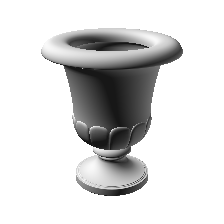
\includegraphics[width=0.11\columnwidth,height=2cm]{figs/real_dataset/Image/jar_d56098d4d83f5976a2c59a4d90e63212.png} &
    	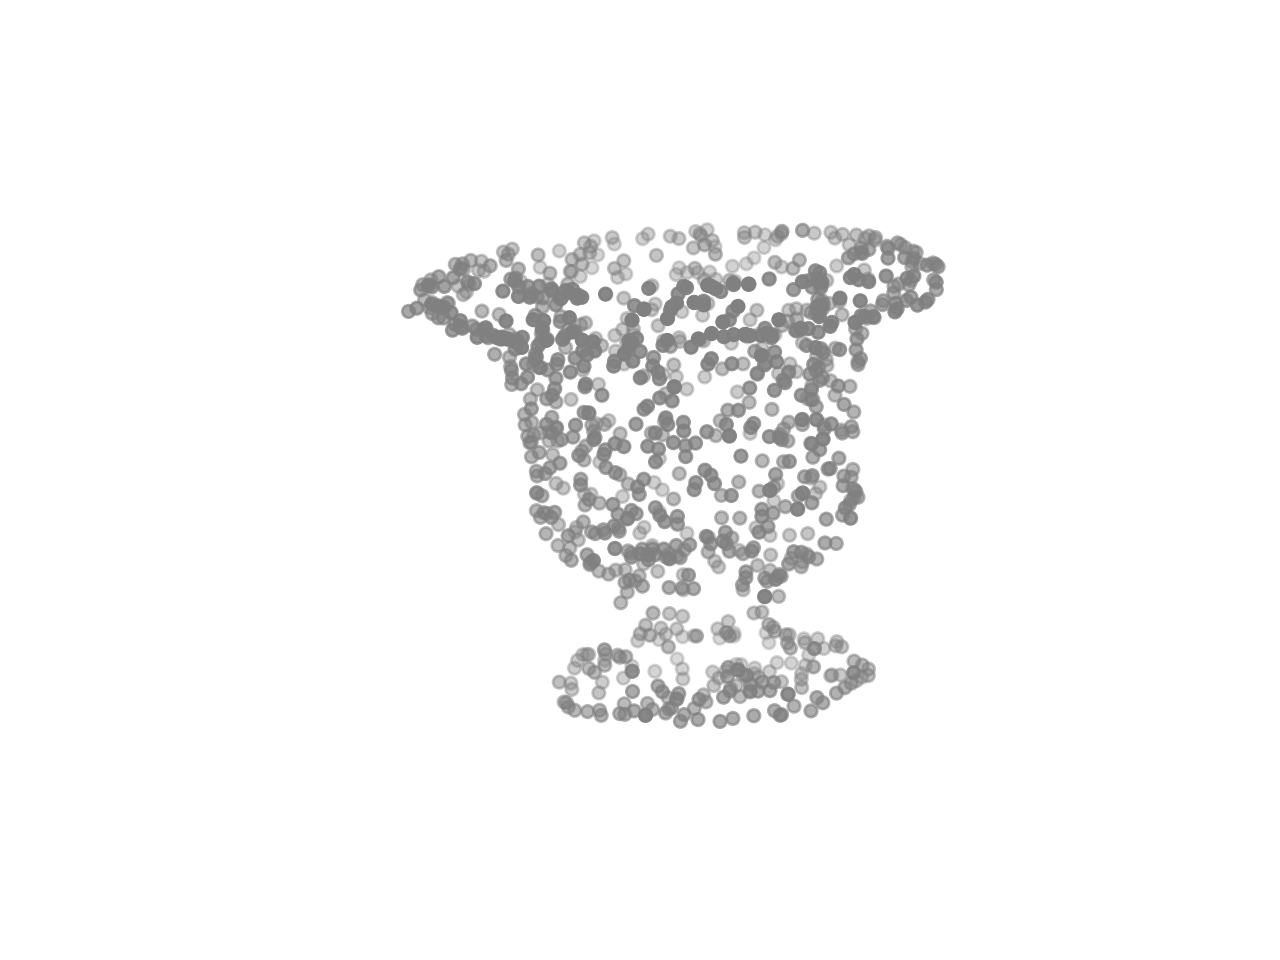
\includegraphics[width=0.22\columnwidth,height=2cm]{figs/real_dataset/GT/jar_d56098d4d83f5976a2c59a4d90e63212_gt.png} &
    	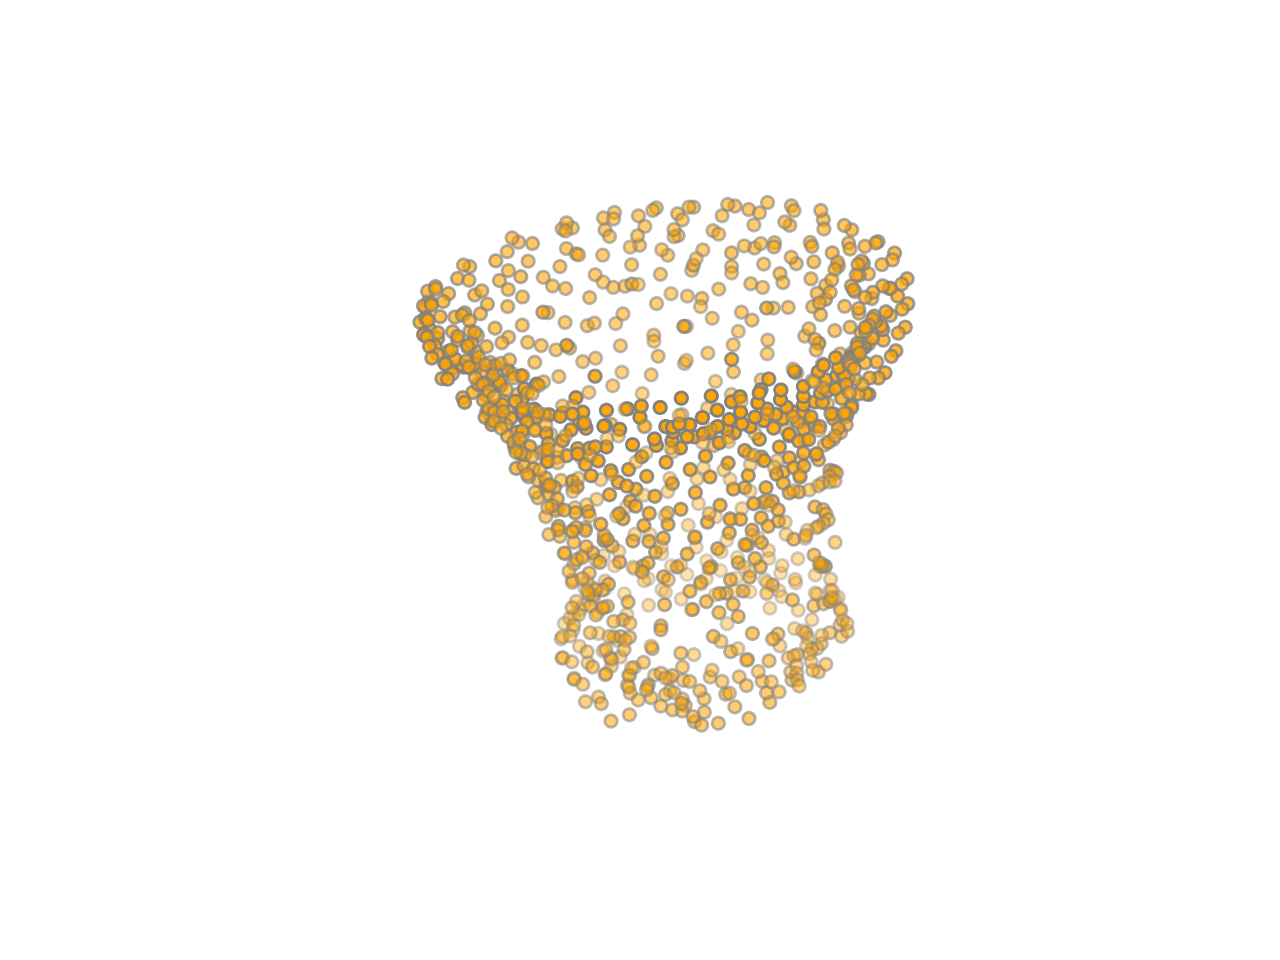
\includegraphics[width=0.22\columnwidth,height=2cm]{figs/real_dataset/AE_label/jar_d56098d4d83f5976a2c59a4d90e63212_fine.png} &
    	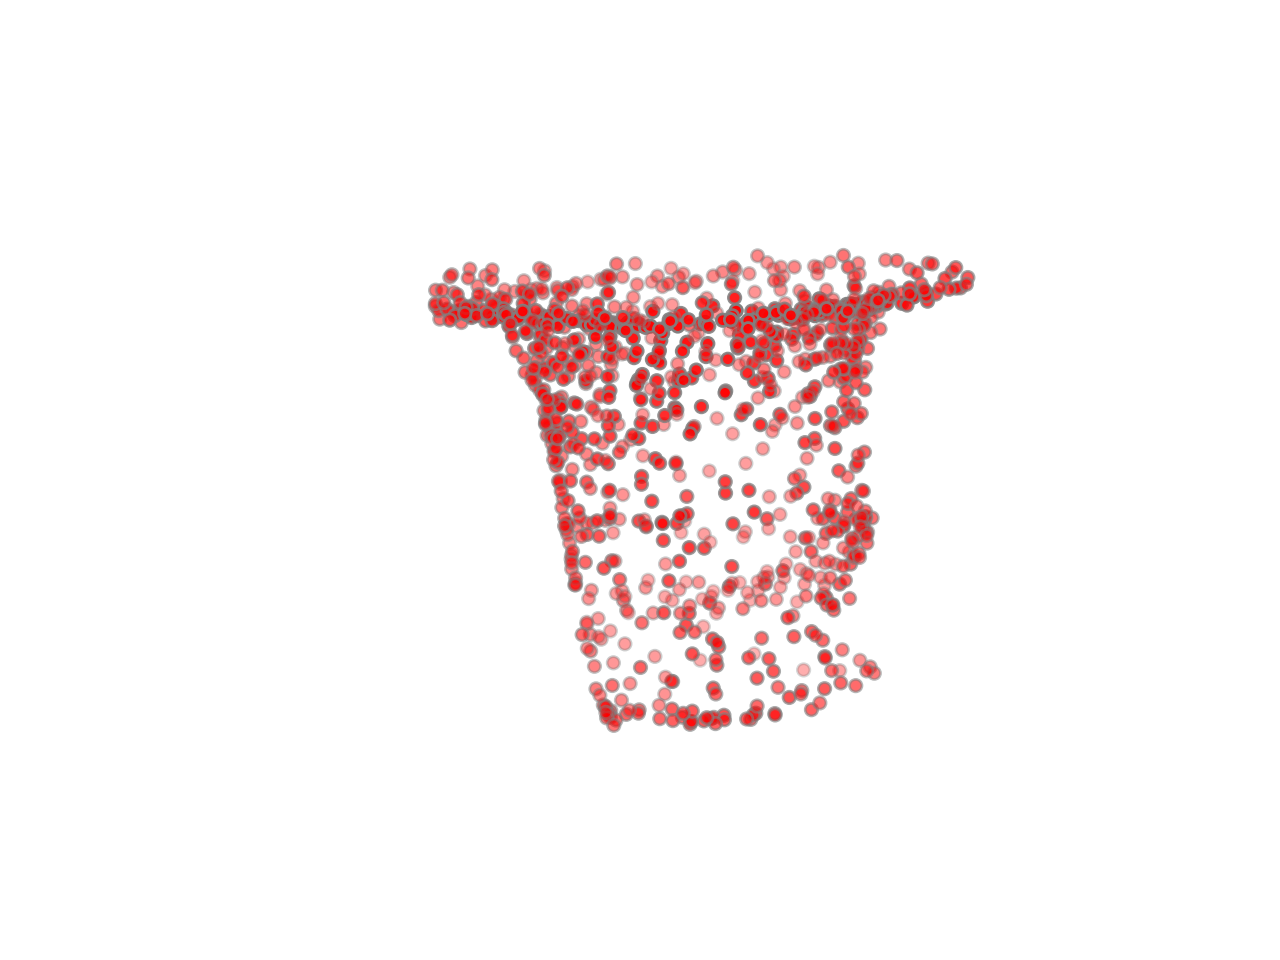
\includegraphics[width=0.22\columnwidth,height=2cm]{figs/real_dataset/AE/jar_d56098d4d83f5976a2c59a4d90e63212_fine.png} &
    	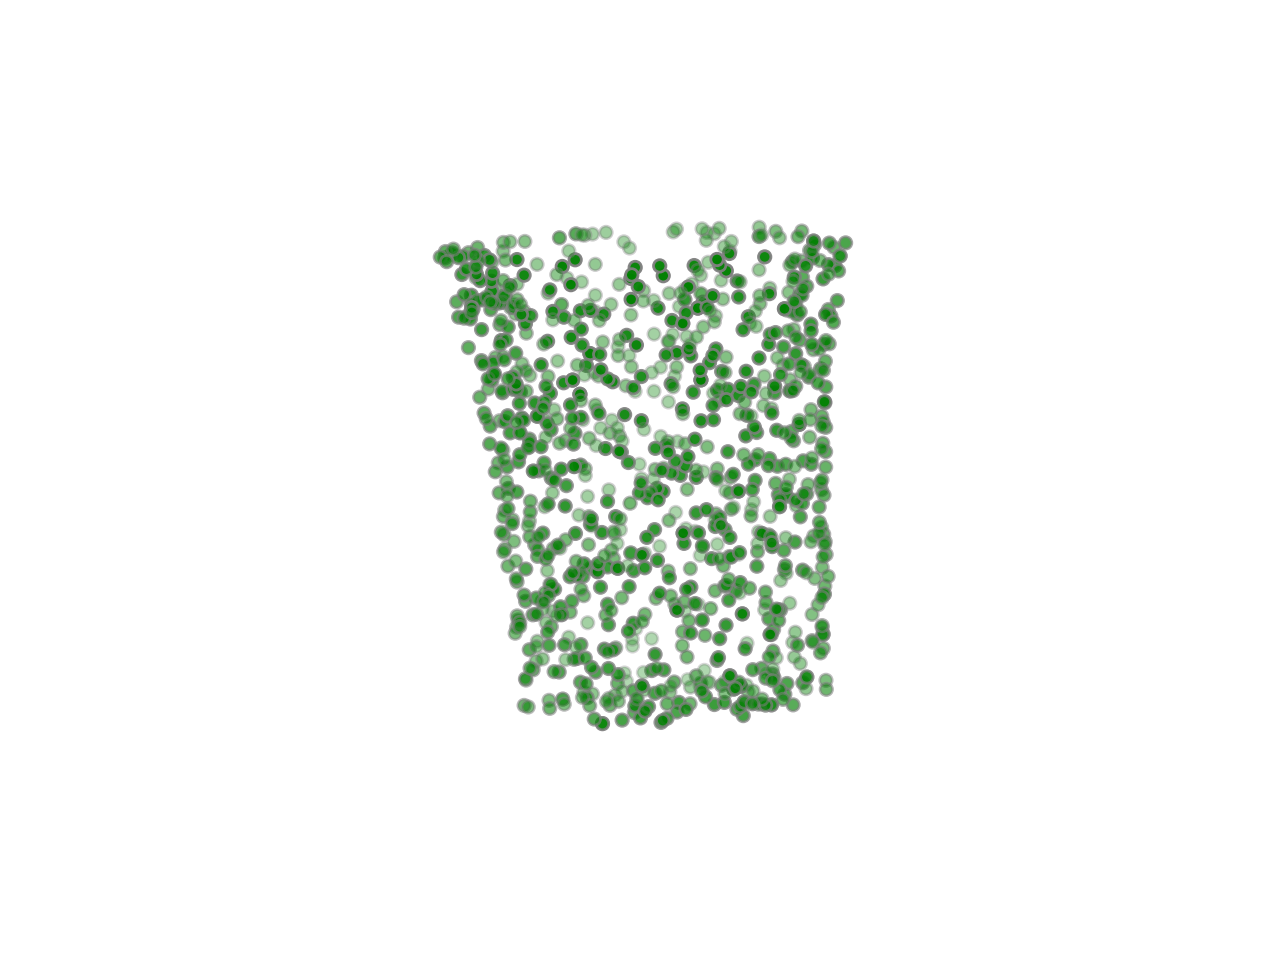
\includegraphics[width=0.22\columnwidth,height=2cm]{figs/real_dataset/oracle/jar_d56098d4d83f5976a2c59a4d90e63212_oracle.png}
    	\\
    \end{tabular}
    \caption{\small 各模型预测结果的可视化}
    \label{fig:visualize_KC}
\end{figure}

\FloatBarrier

\noindent
\textbf{机制探究}

在这个部分,我们证明了在ShapeNet上训练的标准的神经网络执行一个重建任务而不是识别任务。论证理由如下:
\begin{enumerate}
    \item 根据上文部分\ref{sec:shapenet_result}展示的训练结果,由标准的三维重建网络获得的重建结果在量化指标如
    Chamfer Distance和F-score上超过了基于识别机制的非深度学习方法Oracle-NN的重建结果。且Oracle-NN是基于识别机制的非深度学习方法的
    理论极限,因此可以推理出在我们展示的实验中,三维重建神经网络并没有执行识别机制,且基于重建机制的模型在ShapeNet上的性能超越了基于识别机制的模型。
    \item 我们展示了二维T-SNE(见图\ref{fig:TSNE-Chamfer})。图\ref{fig:T-SNE1}和图\ref{fig:T-SNE2}分别展示了在训练时有类标签监督和没有类标签监督
    的两个神经网络的可视化结果(每个模型都训练了100个周期)。T-SNE图上的每个二维点都表示在测试时编码器输出的一个码字。我们只选择了9个样本最多的类,
    因此如果存在聚类效果的话那么这一效果会更明显。这两个神经网络有同样的结构,都使用的是上文优化模型中使用残差层改进解码器后的基准模型\ref{sec:resnet_decoder},并且他们使用同样的流程进行训练(100个周期,学习率0.003,
    批处理大小32,权值衰减1E-6,并且都使用同样的学习率衰减步骤)。

    在图\ref{fig:T-SNE1},神经网络使用类标签监督训练,我们看到清楚的聚类特征同时网络有比较高的Chamfer Distance,也意味着比较差的重建效果。
    相反图\ref{fig:T-SNE2}并没有展现出清楚的聚类特征但有比较低的Chamfer Distance。这个比较说明了分类信息并不总是对三维重建有提升作用。T-SNE比较也是一个
    能够证明标准训练不会导致神经网络执行识别任务的有力证据。
\end{enumerate}

\begin{figure}
	\begin{subfigure}[t]{0.3\linewidth} \centering 
     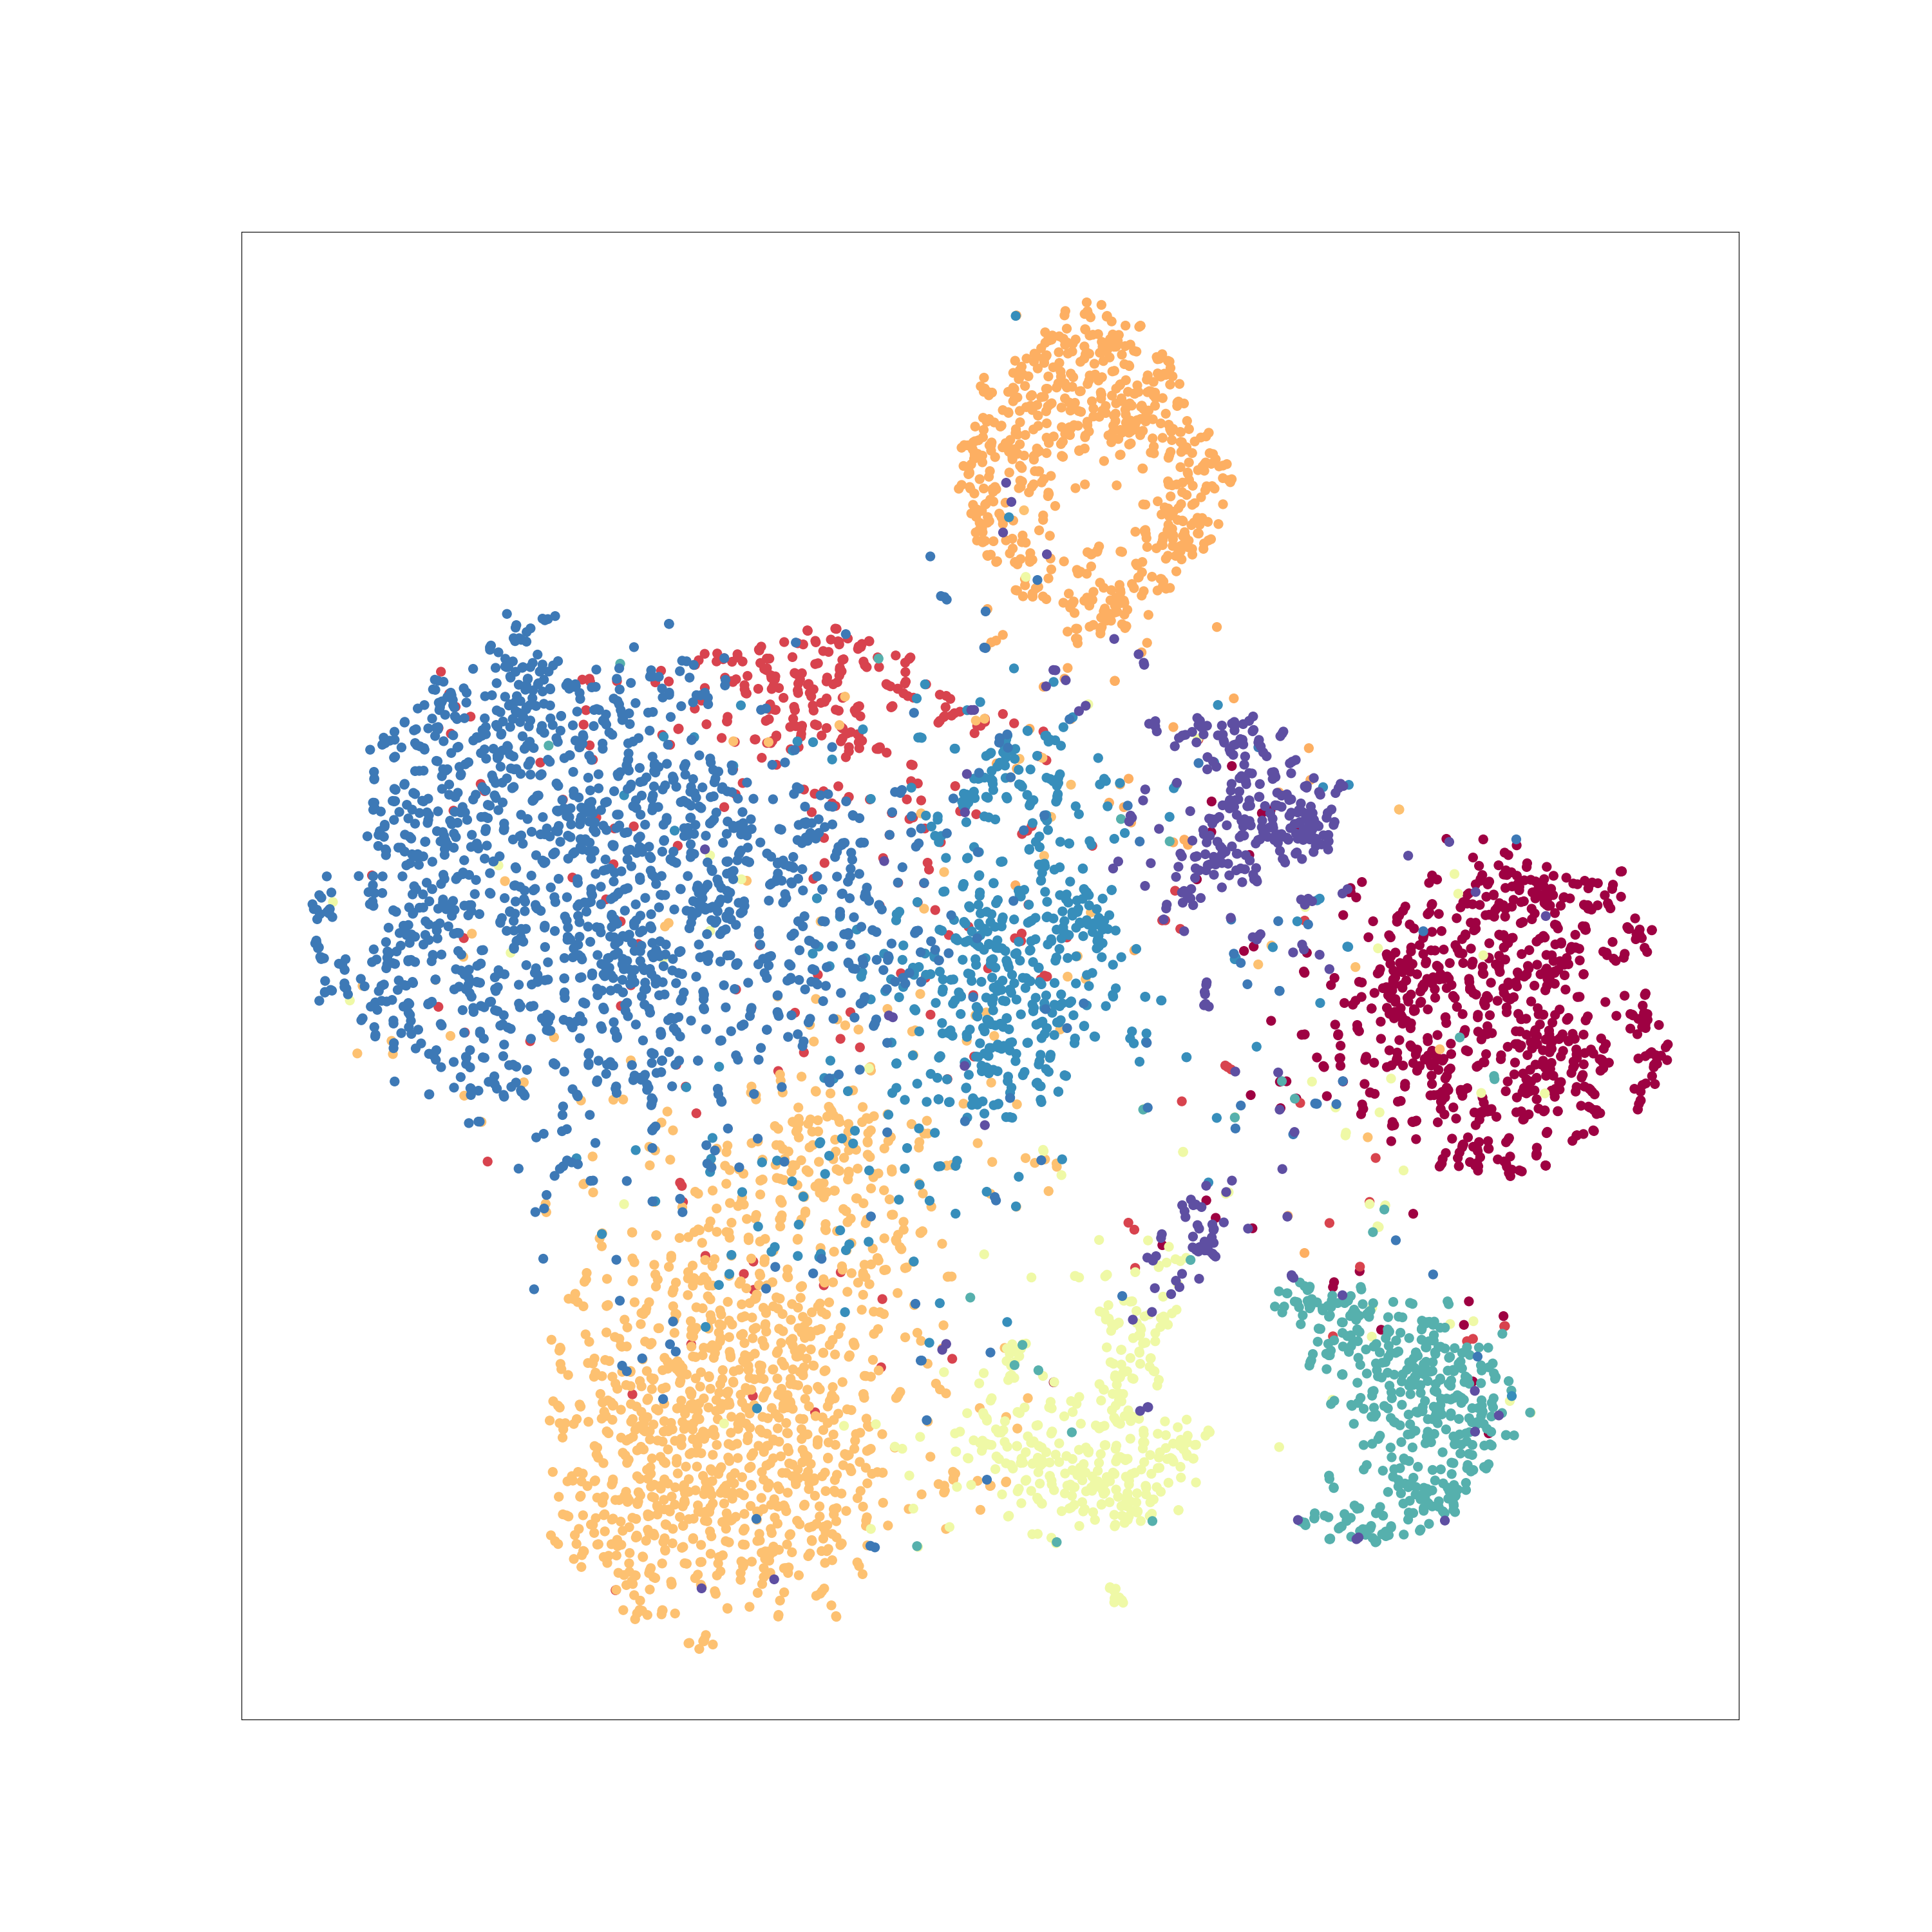
\includegraphics[width=\columnwidth]{figs/T-SNE-class.png}
     \caption{有类标签监督}\label{fig:T-SNE1}
   \end{subfigure}
   \begin{subfigure}[t]{0.3\linewidth} \centering
    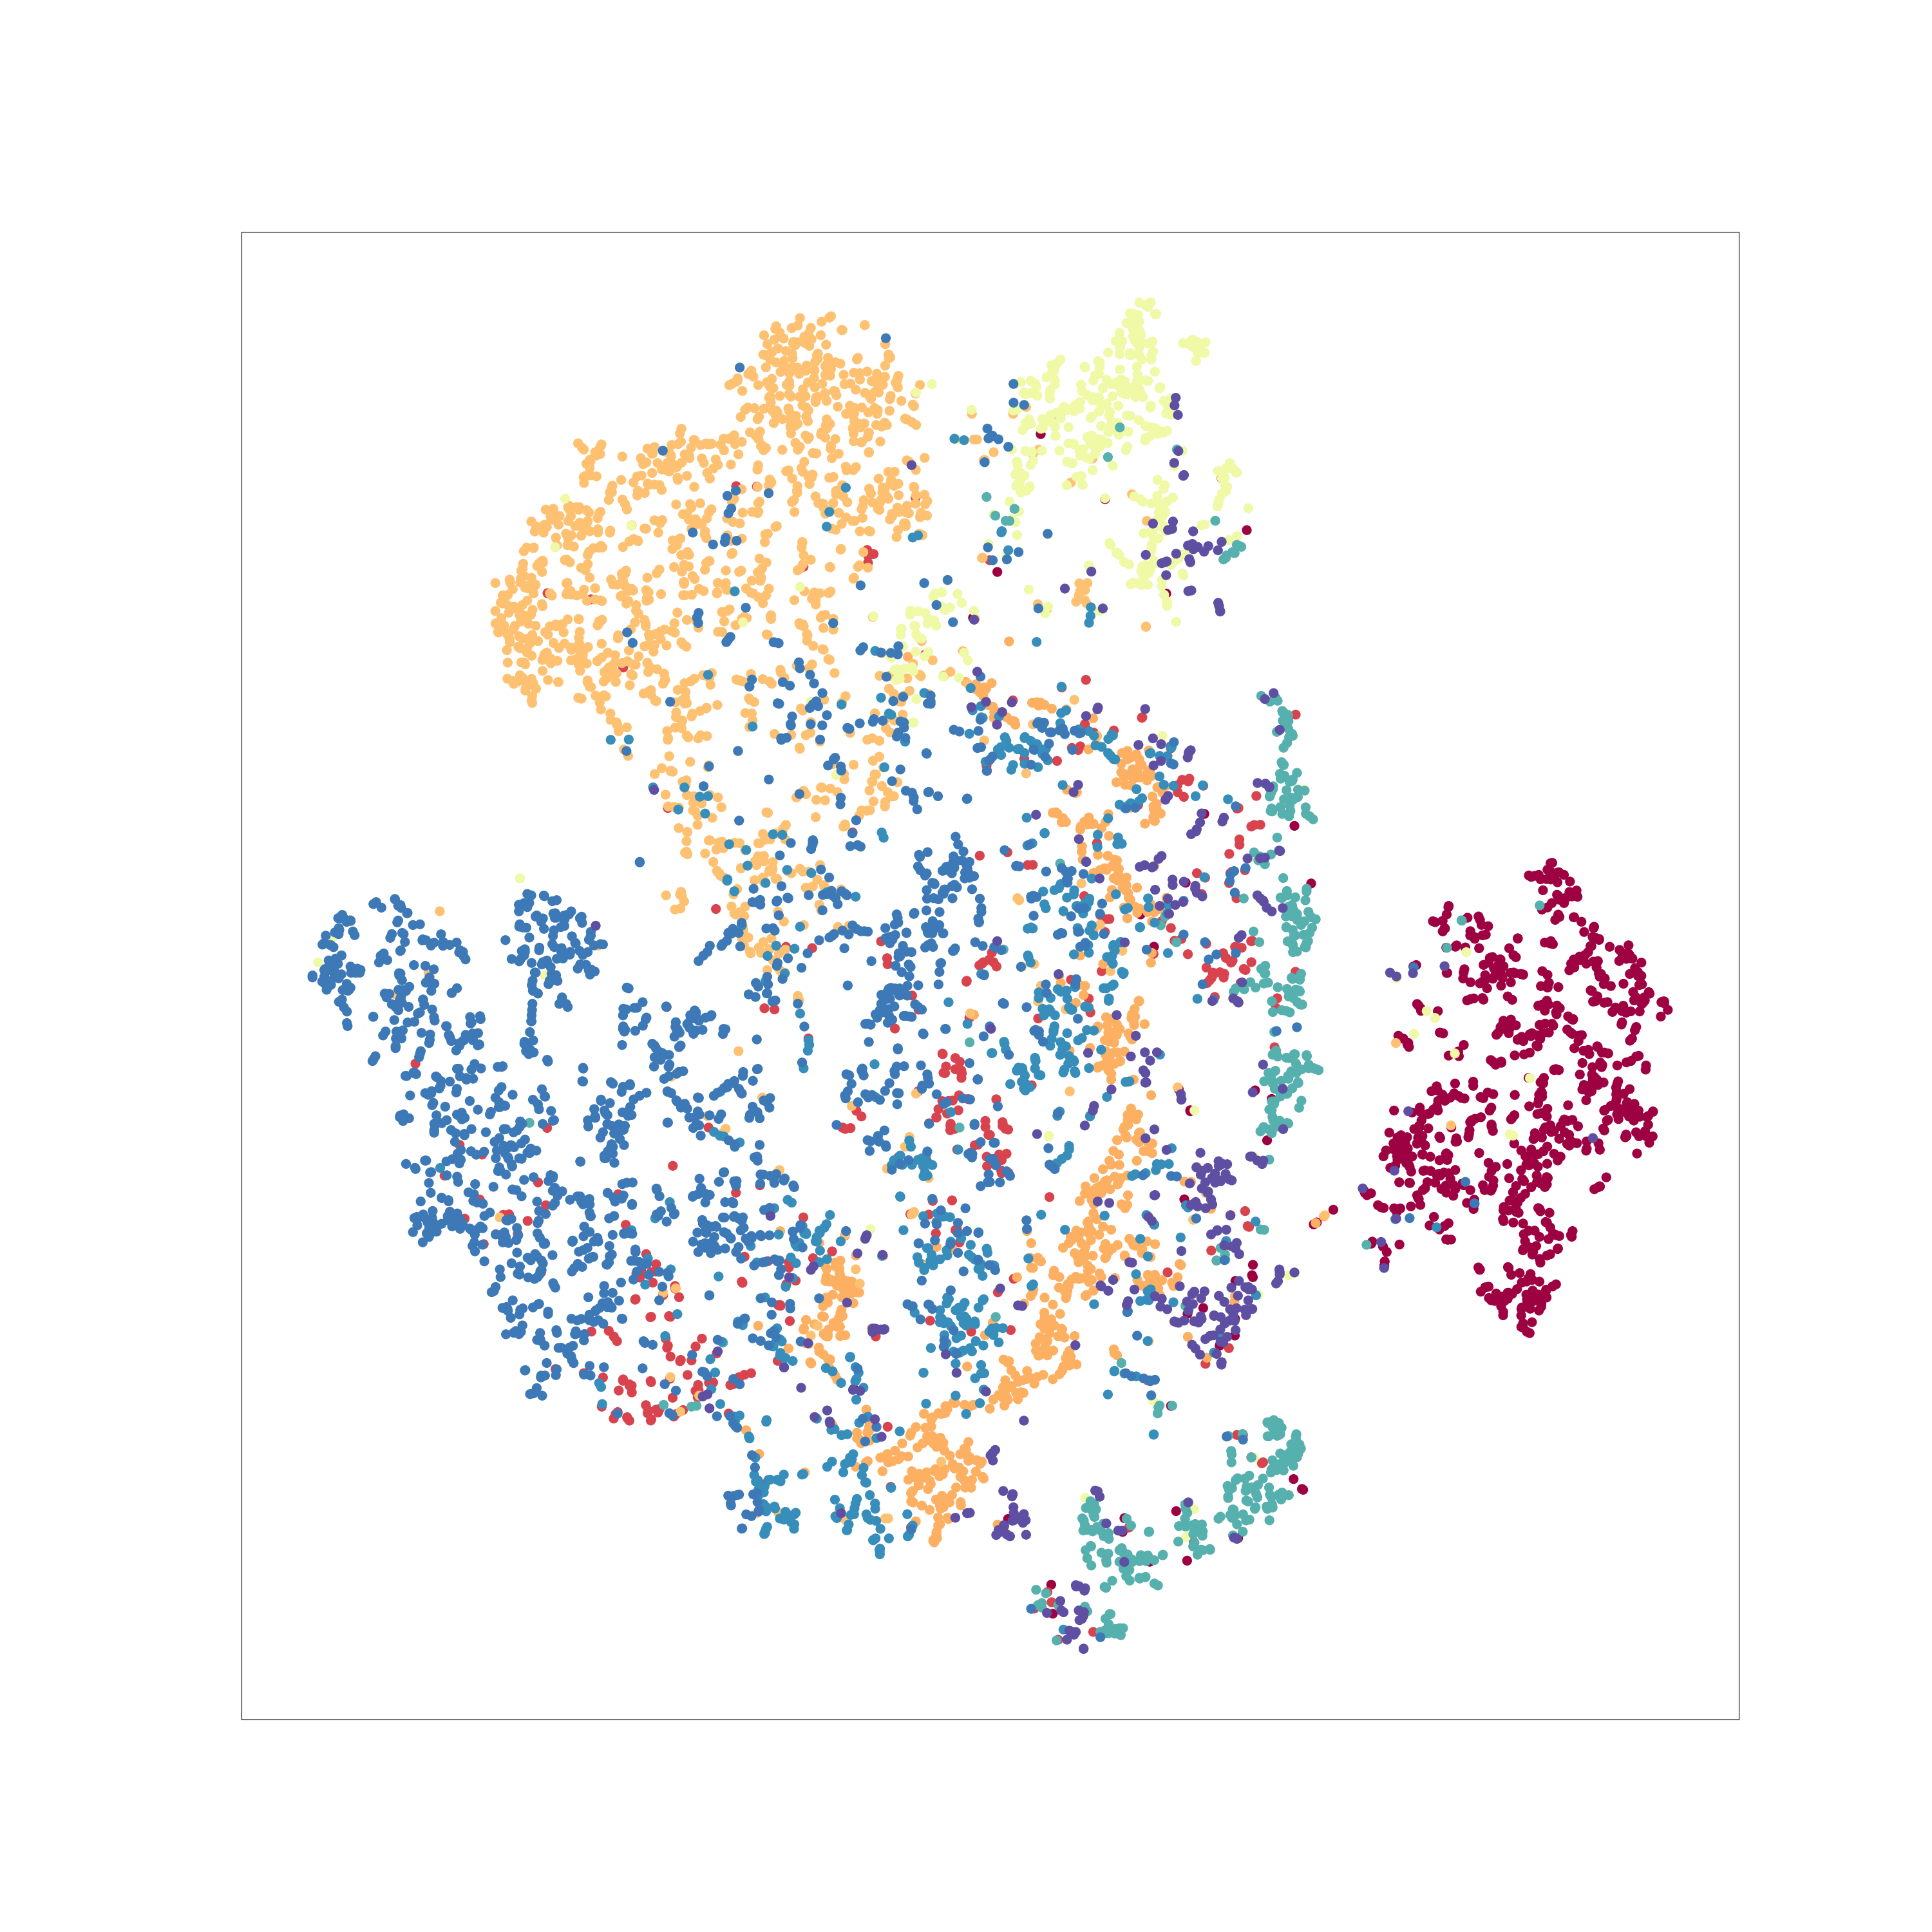
\includegraphics[width=\columnwidth]{figs/T-SNE-noclass.png}
    \caption{没有类标签监督}\label{fig:T-SNE2}
  \end{subfigure}
  \hspace{0.05\linewidth}
  \begin{subfigure}[t]{0.2\linewidth} \centering
    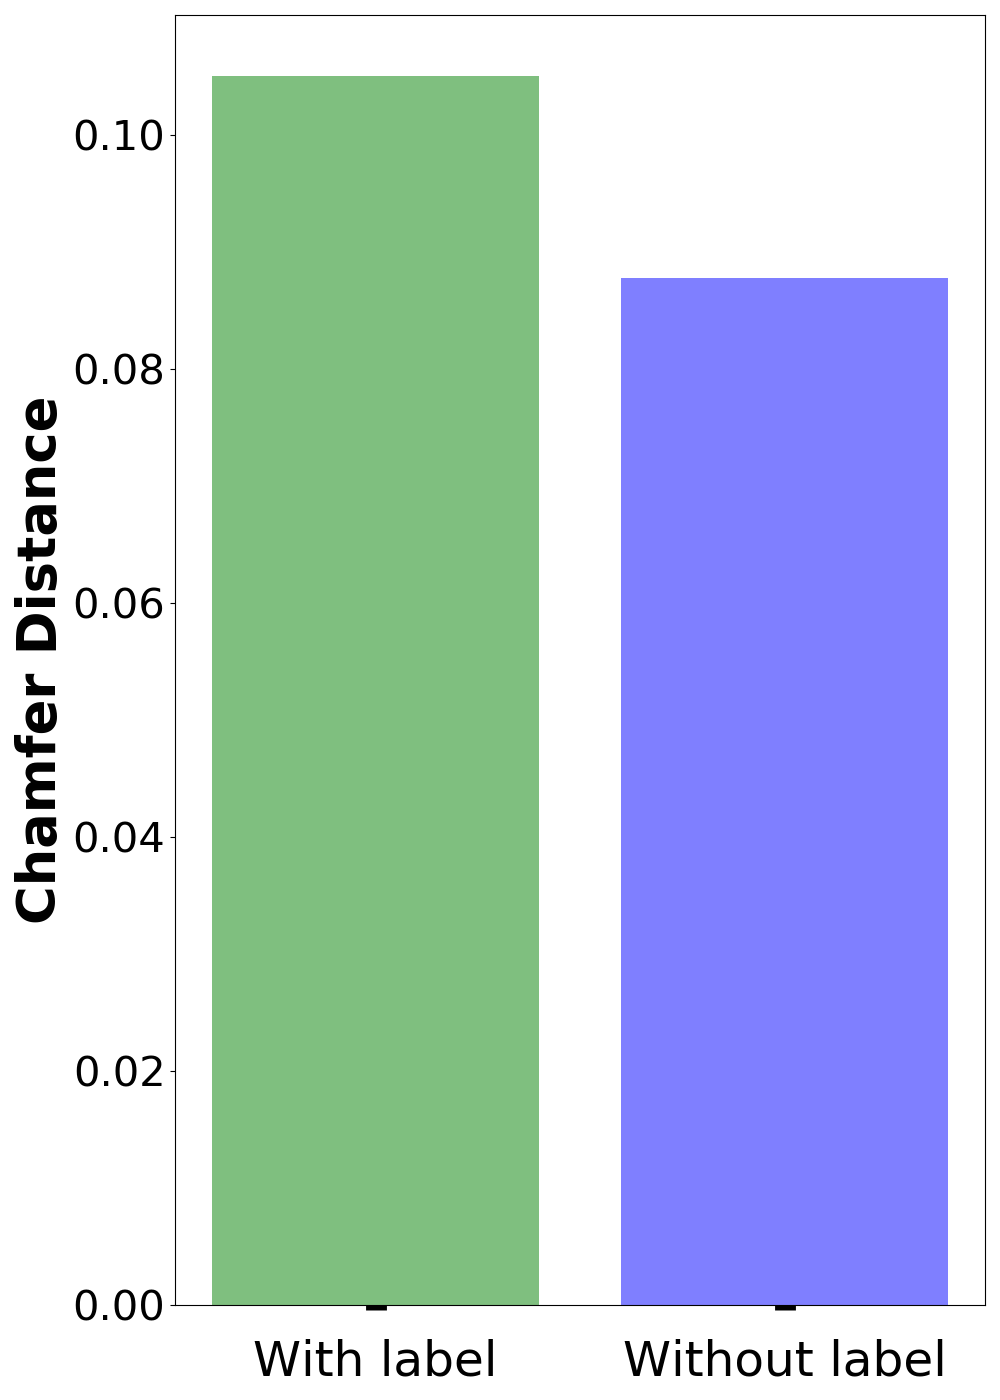
\includegraphics[width=\columnwidth]{figs/label-or-not.png}
    \caption{Chamfer Distance}\label{fig:T-SNE3}
  \end{subfigure}
  \caption{\small 两种训练模式(有类标签监督和没有类标签监督)下的神经网络的T-SNE and Chamfer Distance }\label{fig:T-SNE}
  \label{fig:TSNE-Chamfer}
\end{figure}


\chapter{机制探究}
在这个章节,我们首先理论分析了训练数据的聚类特性与训练后的神经网络在识别机制与重建机制之间偏倚的关联性(可以参考前文章节\ref{sec:recog_or_recon}的定义)。
然后,我们使用在合成数据集上得出的实验结果来支持理论分析(参考章节\ref{sec:dataset})
\section{理论分析}\label{sec:thm}
在这个子章节,我们分析了在三维重建任务中观察到的识别现象背后的直观理解。我们展示了,当训练点云集的聚类趋势比训练图片集的聚类趋势大时,训练后的模型
更倾向于执行识别机制而不是重建机制。参考图\ref{fig:clustering_tendency}。

\begin{figure}
    \centering
    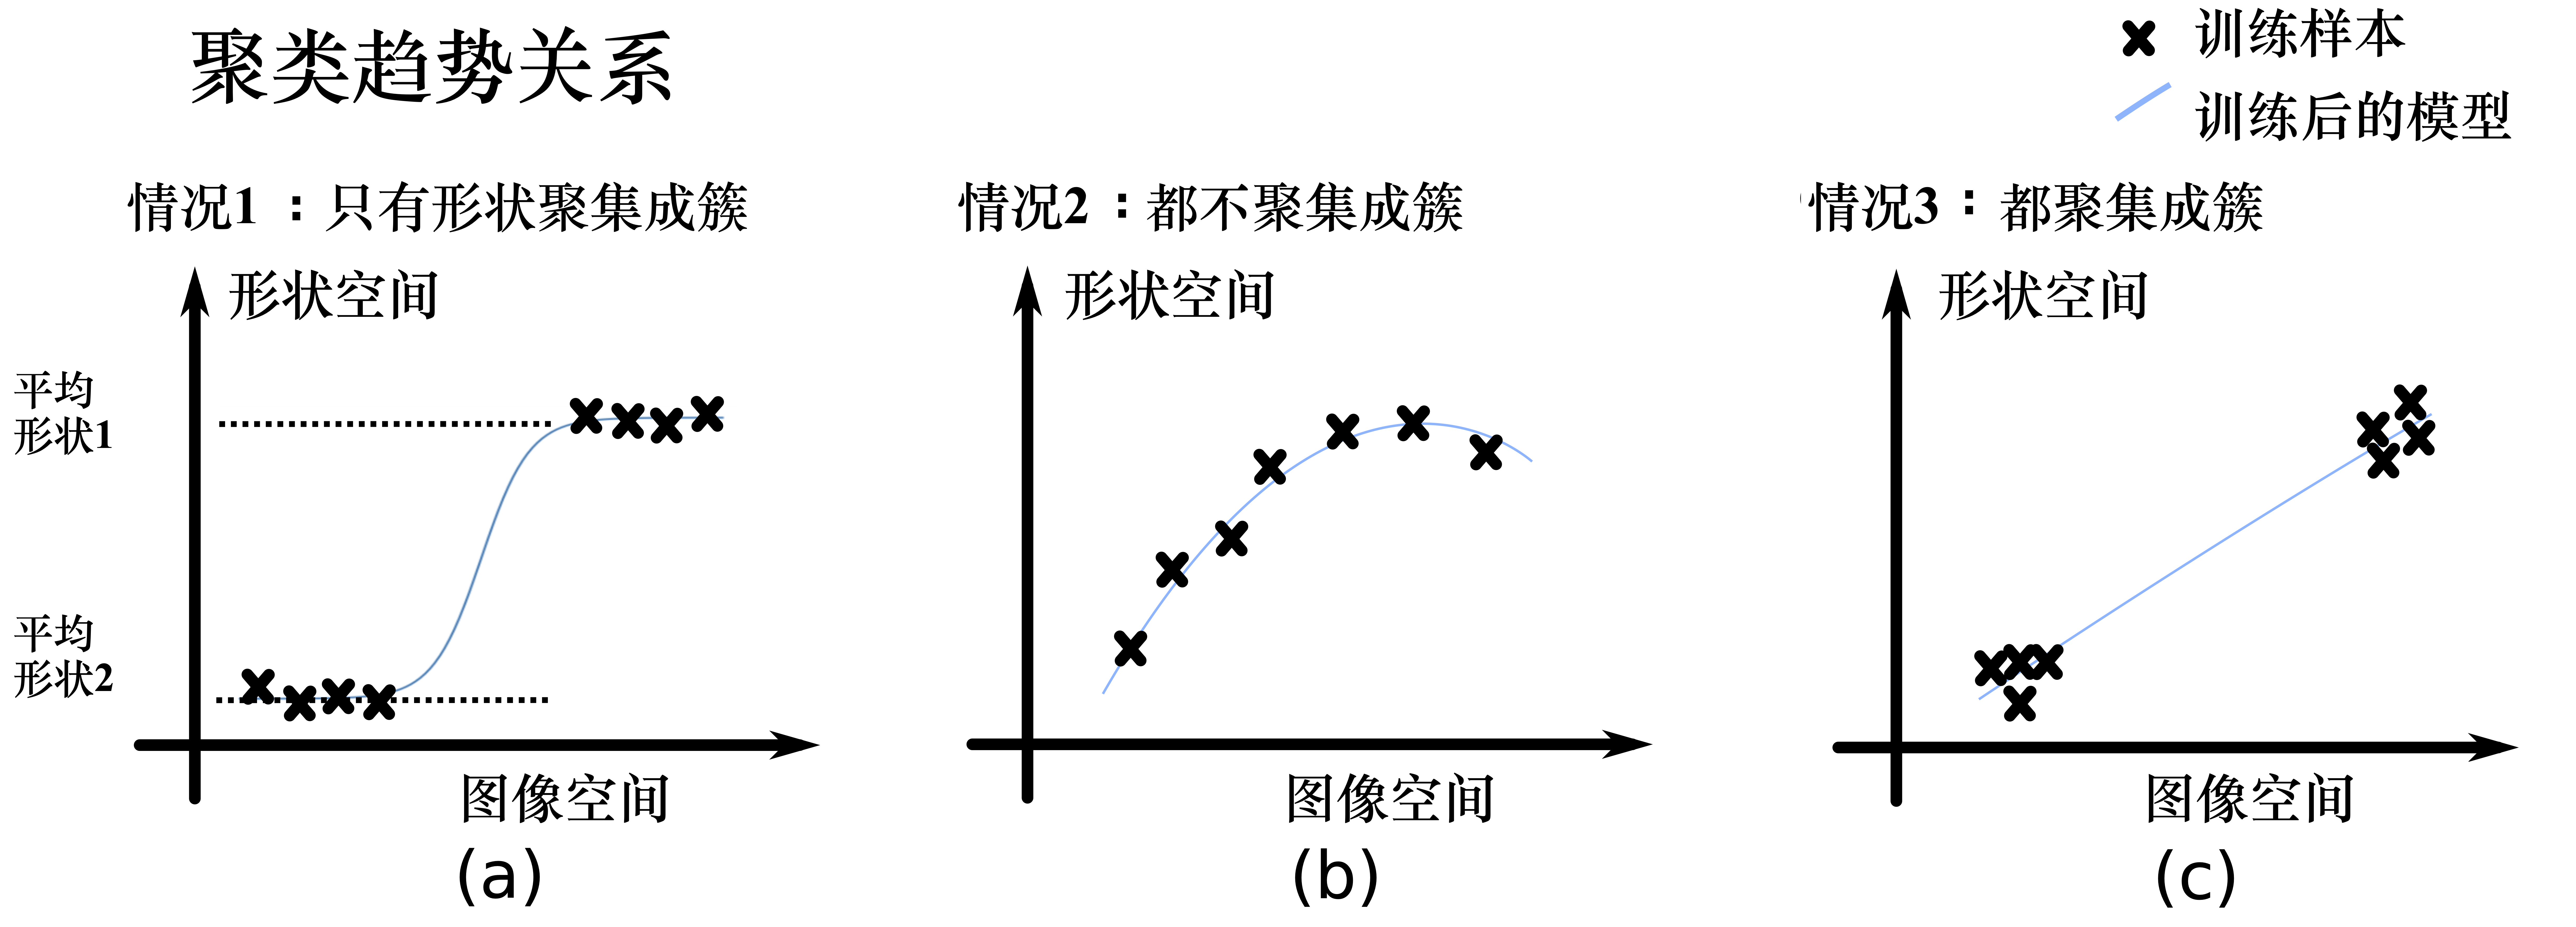
\includegraphics[width=.95\textwidth]{figs/drawing.png}
    \caption{\small 数据集聚类趋势关系}
    \label{fig:clustering_tendency}
\end{figure}

在图\ref{fig:clustering_tendency},我们展示了三种不同类别的训练数据。在子图\ref{fig:clustering_tendency}a,训练图片比训练形状聚类程度更小。
在这种类型数据上训练的模型展示出一个更明显的倾向去执行识别机制,比如形状预测集中在平均形状上,表示为虚线与y轴的交界处。
在子图\ref{fig:clustering_tendency}b,训练图片和训练形状都没有展示出明显的强烈的聚类趋势。所以在这种类型的数据上训练的模型不会执行识别机制。在子图\ref{fig:clustering_tendency}c,
我们展示了另外一种情况,当图片和形状都成簇时,训练后的模型预测的结果不会呈现一个强的聚类趋势。这也许违背直观认知,但是它确实符合我们在实验中观察的现象。

总结一下,列举我们在单视角三维重建实验(从图片到点云形状)中探索的三类数据情况。
\label{sec:case}
\begin{itemize}
    \item[-] 情况1\label{sec:case1}:训练形状集聚集成簇而训练图片集不成簇
    \item[-] 情况2\label{sec:case2}:训练图片集与训练形状集都不聚集成簇
    \item[-] 情况3\label{sec:case3}:训练图片集与训练形状集都聚集成簇
\end{itemize}

我们关于神经网络向识别机制还是重建机制偏倚的观点如下:

\textbf{主要观点}:基于深度学习的单视角三维重建神经网络倾向于只在情况1进行识别,在情况2和情况3进行重建。


\section{实验设计与数据集生成}\label{sec:dataset}

为了证明上一子章节\ref{sec:thm}理论分析中提出的观点,我们需要实验数据集具备不同程度的聚类特征,因此我们需要制造自定义数据集。
在这个子章节,我们提供了合成形状数据集的细节。我们使用软件Blender生成网格形式的基础形状。然后,我们使用“最近顶点”模式的Shrinkwrap
modifier 来定义两个基础形状之间的形变,并且使用Blender Shape Keys面板控制这个插值过程。由此获得的基础数据集中的所有样本的三维形状在数据域中近似均匀分布且连续变化,
这样方便我们采样出具有不同聚类特征的子数据集。我们渲染训练图片并且
从网格上采样点云形成样本对(图片,点云)以完成基础数据集的创建。之后,我们对基础数据集进行二次采样
获得聚类程度不同的小数据集,以覆盖子章节\ref{sec:thm}提到的情况1,2,3。

\textbf{基础数据集 \#1}(正立方体-球)~第一个基础数据集通过在一个正立方体和一个有相似大小的球之间插值获得。
参考图\ref{fig:cube-sphere}。我们在两端之间插值1000个过渡形状。 对于每个过渡形状,我们从等距视角渲染一张图片并且采样获得一个包含有
1024个三维点的点云表示。1000个过渡形状被随机划分为700个训练形状,200个测试形状以及100个验证形状。


\begin{figure}
	\begin{tabular}{c@{}c@{}c@{}c@{}c@{}c@{}c@{}c@{}c@{}c@{}c@{}}
	    球   & & & & & $\Longleftrightarrow$ & & & & & 正立方体 \\
		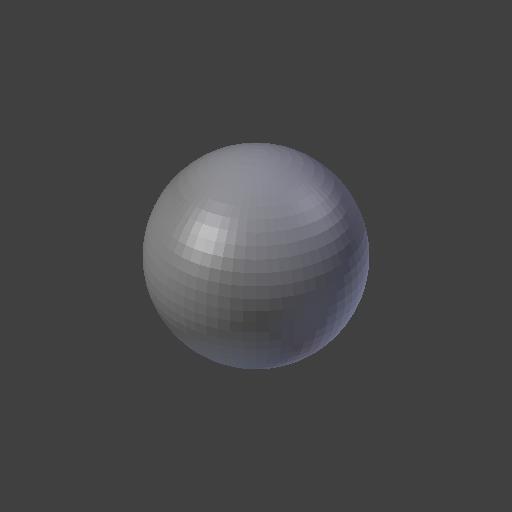
\includegraphics[width=.09\textwidth,keepaspectratio]{figs/Isometric0.png} &
		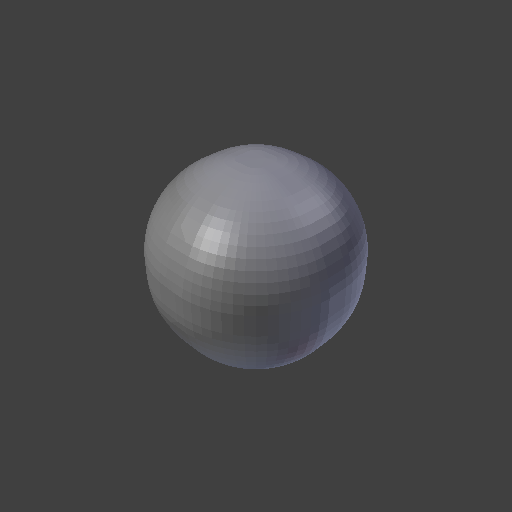
\includegraphics[width=.09\textwidth,keepaspectratio]{figs/Isometric1.png} &
		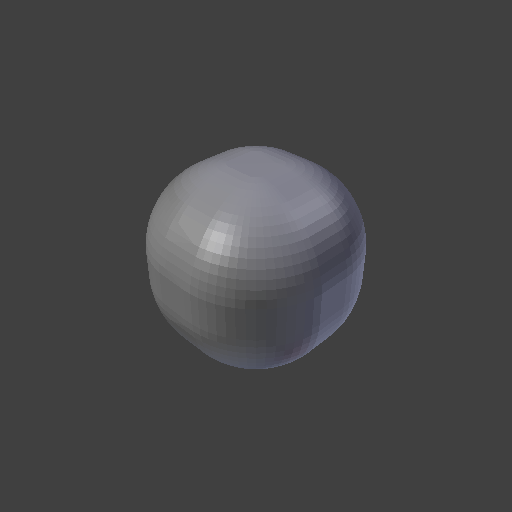
\includegraphics[width=.09\textwidth,keepaspectratio]{figs/Isometric2.png} &
		\includegraphics[width=.09\textwidth,keepaspectratio]{figs/Isometric3.png} &
		\includegraphics[width=.09\textwidth,keepaspectratio]{figs/Isometric4.png} &
		\includegraphics[width=.09\textwidth,keepaspectratio]{figs/Isometric5.png} &
		\includegraphics[width=.09\textwidth,keepaspectratio]{figs/Isometric6.png} &
		\includegraphics[width=.09\textwidth,keepaspectratio]{figs/Isometric7.png} &
		\includegraphics[width=.09\textwidth,keepaspectratio]{figs/Isometric8.png} &
		\includegraphics[width=.09\textwidth,keepaspectratio]{figs/Isometric9.png} &
		\includegraphics[width=.09\textwidth,keepaspectratio]{figs/Isometric10.png} \\    	
	\end{tabular}
	\caption{\small 基础数据集 \# 1}
    \label{fig:cube-sphere} \vspace{-4mm}
\end{figure}

\textbf{二次采样数据集1.1 描述章节\ref{sec:case2}的情况2和情况3} ~创建二次采样数据集1.1目的是覆盖从情况2到情况3的转化。这个数据集是一组7个二次采样数据集的集合1.1.n(n=1,2,$\ldots$7)。
每个二次采样数据集1.1.n包含了5个形状簇和相应的图片。从二次采样数据集1.1.1到二次采样数据集1.1.7,聚集趋势逐渐变低。
更具体的是,二次采样数据集1.1.1五个分离的簇(参考图\ref{fig:five-clusters}第一列),同时二次采样数据集1.1.7几乎
连续覆盖了从球到正立方体的整个变化(参考\ref{fig:two-clusters})。需要注意的是全部的七个二次采样数据集包含了相同数量的训练图片,比如每个数据集
包含五个簇,每个簇包含20个样本。但是每个二次采样数据集的测试集保持与基础数据集1的测试集一样。换句话说,我们只对训练集进行二次采样,同时保持固定的
测试集。

\textbf{二次采样数据集1.2 描述章节\ref{sec:case1}的情况1和情况3} ~二次采样数据集1.2是基础数据集1的另一个二次采样
版本。这个数据集的目的是覆盖从情况1到情况3的转变。这个数据集是一个7个二次采样数据集1.2.n(n=1,2,$\ldots$7)的集合。每个数据集1.2.n包含了
两个样本簇。但是,与二次采样数据集1.1不同,尽管二次采样数据集1.2中的每个训练对(图片,三维形状)有一个独特的二维图片,相对应的三维形状
只能为两个端点形状中的其中一个(例如两个基础形状正立方体和球),并且没有过渡形状存在。所以在这种情况下,训练形状的聚类趋势总是非常高,同时
从二次采样数据集1.2.1到1.2.7的训练图片的聚类趋势逐渐变低。与之前一样,二次采样数据集1.2.7的训练图片集几乎覆盖了从球到正立方体的整个
变化。所以,二次采样数据集1.2.1表示了情况3的一个案例,同时1.2.7表示了情况1的一个案例并且数据集1.2.n(n = 1,2,$\ldots$7)表示了
从情况3到情况1的转变。在每个数据集,训练图片的数量总是$2\times10$,2是簇的数量,10是每个簇的样本数量。与二次采样数据集1.1相似,
二次采样数据集1.2的测试集依然是基础数据集1的测试集。

\begin{figure}
	\begin{subfigure}[t]{0.45\linewidth} \centering 
     \includegraphics[width=\columnwidth]{figs/five-clusters.png}
     \caption{\small 数据集 1.1.n (n = 1, 2, $\ldots $7)。不同的二次采样数据集有不同的聚簇趋势。}\label{fig:five-clusters}
   \end{subfigure}\hspace{0.05\textwidth}
   \begin{subfigure}[t]{0.45\linewidth} \centering
     \includegraphics[width=\columnwidth]{figs/two-clusters.png}
     \caption{\small 数据集 1.2.n (n = 1, 2, $\ldots $7). 点标记代表图像分布,同时叉标记代表点云分布。}\label{fig:two-clusters}
   \end{subfigure}
   \caption{\small 二个二次采样的数据集 1.1.n 和 1.2.n 在基础数据集上的分布}
\end{figure}

\textbf{基础数据集 \#2}(正立方体-正四面体-球)~为了增加合成数据集的复杂度,增加实验验证的有效性,我们生成了一个比基础数据集\#1更复杂的数据集,在三个基础形状之间插值,分别是
正立方体,正四面体,球。这三个形状有相似的大小。在这三个基础形状之间,我们插值了10000个过渡形状。与基础数据集\#1相似,我们从基础数据集\#2中创造了
二次采样数据集来表现在章节\ref{sec:thm}中讨论的不同情况。具体来说,我们首先使用了正四面体和正立方体作为两个基础形状并生成了100个过渡
形状$S_1,S_2,\ldots S_{100}$,然后,我们选择每个基础过渡形状$S_i$,并且在$S_i$和基础形状球之间线性插值100个形状。
这个二维插值的过程总共给了我们$100 \times 100 = 10000$个过渡形状。这10000个形状再次被分为7000个训练样本,
1000个验证样本和2000个测试样本。 

\begin{figure}
	\begin{tabular}{c@{}c@{}c@{}c@{}c@{}c@{}c@{}c@{}c@{}c@{}c@{}}
	    正立方体   & & & & & $\Longleftrightarrow$ & & & & & 正四面体 \\
		\includegraphics[width=.09\textwidth,keepaspectratio]{figs/triangle/cube_triangle/Isometric_0.png} &
		\includegraphics[width=.09\textwidth,keepaspectratio]{figs/triangle/cube_triangle/Isometric_1.png} &
		\includegraphics[width=.09\textwidth,keepaspectratio]{figs/triangle/cube_triangle/Isometric_2.png} &
		\includegraphics[width=.09\textwidth,keepaspectratio]{figs/triangle/cube_triangle/Isometric_3.png} &
		\includegraphics[width=.09\textwidth,keepaspectratio]{figs/triangle/cube_triangle/Isometric_4.png} &
		\includegraphics[width=.09\textwidth,keepaspectratio]{figs/triangle/cube_triangle/Isometric_5.png} &
		\includegraphics[width=.09\textwidth,keepaspectratio]{figs/triangle/cube_triangle/Isometric_6.png} &
		\includegraphics[width=.09\textwidth,keepaspectratio]{figs/triangle/cube_triangle/Isometric_7.png} &
		\includegraphics[width=.09\textwidth,keepaspectratio]{figs/triangle/cube_triangle/Isometric_8.png} &
		\includegraphics[width=.09\textwidth,keepaspectratio]{figs/triangle/cube_triangle/Isometric_9.png} &
		\includegraphics[width=.09\textwidth,keepaspectratio]{figs/triangle/cube_triangle/Isometric_10.png} \\    	
    \end{tabular}
    \begin{tabular}{c@{}c@{}c@{}c@{}c@{}c@{}c@{}c@{}c@{}c@{}c@{}}
	    球   & & & & & $\Longleftrightarrow$ & & & & & 插值形状 \\
		\includegraphics[width=.09\textwidth,keepaspectratio]{figs/triangle/sphere_triangle/Isometric0.png} &
		\includegraphics[width=.09\textwidth,keepaspectratio]{figs/triangle/sphere_triangle/Isometric1.png} &
		\includegraphics[width=.09\textwidth,keepaspectratio]{figs/triangle/sphere_triangle/Isometric2.png} &
		\includegraphics[width=.09\textwidth,keepaspectratio]{figs/triangle/sphere_triangle/Isometric3.png} &
		\includegraphics[width=.09\textwidth,keepaspectratio]{figs/triangle/sphere_triangle/Isometric4.png} &
		\includegraphics[width=.09\textwidth,keepaspectratio]{figs/triangle/sphere_triangle/Isometric5.png} &
		\includegraphics[width=.09\textwidth,keepaspectratio]{figs/triangle/sphere_triangle/Isometric6.png} &
		\includegraphics[width=.09\textwidth,keepaspectratio]{figs/triangle/sphere_triangle/Isometric7.png} &
		\includegraphics[width=.09\textwidth,keepaspectratio]{figs/triangle/sphere_triangle/Isometric8.png} &
		\includegraphics[width=.09\textwidth,keepaspectratio]{figs/triangle/sphere_triangle/Isometric9.png} &
		\includegraphics[width=.09\textwidth,keepaspectratio]{figs/triangle/sphere_triangle/Isometric10.png} \\    	
	\end{tabular}
	\caption{\small 基础数据集 \# 2}
    \label{fig:cube-sphere} \vspace{-4mm}
\end{figure}

\textbf{二次采样数据集2.1 描述章节\ref{sec:case2}的情况2和情况3} ~二次采样数据集2.1的目的是覆盖从情况2到情况3的变化。这个数据集是一组6个二次采样数据集的集合2.1.n(n=1,2,$\ldots$6)。
从二次采样数据集2.1.1到2.1.6,聚集趋势逐渐变低。
更具体的是,二次采样数据集2.1.1有三个明显分离的簇,由在三个基础形状周围采样获得,同时二次采样数据集2.1.6几乎
连续覆盖了从2.1.1到2.1.6的所有变化。每个二次采样数据集有三个簇,每个簇有30个样本。与正立方体-球数据集$\#$1相似,测试集保持固定(是基础数据集$\#$2的
初始测试集)。但是,因为测试集里的形状数量非常多,我们对测试集通过随机选择300个测试样本进行了二次采样。当训练神经网络时,我们使用了验证数据集来选择最优的
模型。

\textbf{二次采样数据集2.2 描述章节\ref{sec:case1}的情况1和情况3} ~二次采样数据集2.2的目的是覆盖从情况3到情况1的变化。它包含了六个数据集
2.2.n(n=1,2,$\ldots$6)。从二次采样数据集2.2.1到2.2.6,训练图片集的聚类趋势逐渐降低,同时训练点云集的聚类趋势保持在高水平。
我们固定训练点云,比如对于每个样本对$(I,S)$,我们使得与每个训练图片$I$相关的训练点云$S$都是三个基础形状中的一个。
所以,从二次采样数据集2.2.1到2.2.6的转变表示了从情况3到情况1的转变。在每个二次采样数据集中,我们生成接近三个基础
形状的簇,并且每个簇有16个样本。当训练神经网络时,我们不使用验证集,并且简单的选择最后一个周期的模型参数。原因是在当前的设定下,
从训练集(只有三个基础形状点云)到验证集(插值形状点云)存在一个域的转变。所以,验证数据集在训练时不能用于选择最优
模型参数。


\section{实验结果}
在这个子章节,我们展示了实验结果来论证\ref{sec:thm}中的主要论点:识别机制只会在训练图片聚簇程度小于训练形状聚簇程度时才会发生,例如,情况1。
为了证明这个论点,我们已经在章节\ref{sec:dataset}中创建了不同的数据集来覆盖情况1,2和3之间的过渡转变。
关于神经网络模型,我们采用了在章节\ref{sec:optimal_method}中使用残差层优化过的自编码器架构\ref{fig:resnet_decoder},
采用Chamfer Distance作为损失函数。对于二次采样数据集1.1,我们为从1.1.1到1.1.7的每个数据集都分别训练了一个单独的神经网络,进行了
1500个周期的训练,以到达保证他们的学习能力饱和。对于子数据集1.2,我们也分别在每个子数据集1.2.n上训练一个单独的神经网络,但训练周期更多,有3000个周期,因为1.2.n每个数据集的样本量
更小。在训练期间,我们使用Adam优化器,初始化学习率为0.003,学习率衰减为0.1。我们使用验证集来选择最好的模型用于预测。

\subsection{数据集指标测量}\label{sec:metric_result}
在这个子章节,我们使用\ref{sec:metric_on_dataset}提出的衡量数据集聚类程度的指标来对我们机制探究实验中所有数据集以及网络预测结果的聚类程度进行测量。

\textbf{基础数据集\#1的实验结果}~在这个部分,我们展示了基础数据集\#1的量化实验结果来支持章节\ref{sec:thm}中的主要观点。对于每个二次采样数据集,我们画出模型输入数据的聚类趋势与输出数据的聚类趋势,由\ref{sec:metric_on_dataset}我们
提出的轮廓系数(silhouette score)表示。因为我们有两类输入数据——训练图片与训练形状,我们分别画出“输入图片-预测结果”和“输入形状-预测结果”这两个关系。结果展示在图\ref{fig:silhouette-dataset-1.png}。
第一行的结果关于二次采样数据集1.1,即从情况3到情况2的转变,同时第二行的结果关于二次采样数据集1.2,即从情况3到情况1的转变。对于二次采样数据集1.1
的结果,即使是输入的聚类趋势变化,输出的聚类趋势保持不变。这一结果证明了我们在\ref{fig:clustering_tendency}b和\ref{fig:clustering_tendency}c
的理论分析,即在情况2和情况3下输出的聚类趋势比较低,神经网络执行重建机制。但是,在图\ref{fig:silhouette-dataset-1.png}的第二行,我们可以看到当输入图片聚类趋势降低时,输出聚类趋势明显
提升。这正是与我们在图\ref{fig:clustering_tendency}a中的理论分析一致,即重建形状的聚簇只会在训练图片不聚簇且训练形状聚簇的情况发生、
注意在第二行,训练形状只包含两个端点形状(球和正立方体)。所以,训练形状的聚类趋势总是非常高(注意图\ref{fig:silhouette-dataset-1.png}第二行
右边的图片)。

\begin{figure}[h!]
    \centering
    \includegraphics[width=.95\textwidth]{figs/silhouette-dataset-1.png}
    \caption{\small “基础数据集\#1的训练图片/形状点云-输出形状”的轮廓系数(silhouette score)。只有情况1(左下角子图中较大的数据集索引指向的点)展示出高的聚类趋势}
    \label{fig:silhouette-dataset-1.png}
\end{figure}
\FloatBarrier
\textbf{基础数据集\#2的实验结果}~在这个部分,我们展示了基础数据集\#2的量化实验结果,该实验结果由在每个二次采样数据集上(2.1.n以及2.2.n)
进行训练和测试获得。具体来说,该量化结果为输入与输出的轮廓系数(silhouette score),展示在图\ref{fig:silhouette-dataset-2.png}。从该图的第二行左侧的图
可以看出只有在情况1预测结果才会呈现出明显的聚类趋势,与章节\ref{sec:thm}的结论一致。该图第一行的两张子图展示了在情况2和情况3下预测结果都不会呈现出
高的聚类趋势。

\begin{figure}[h!]
    \centering
    \includegraphics[width=.95\textwidth]{figs/silhouette-dataset-2.png}
    \caption{\small “基础数据集\#2的训练图片/形状点云-输出形状”的(silhouette score)。只有情况1(左下角子图中较大的数据集索引指向的点)展示出高的聚类趋势}
    \label{fig:silhouette-dataset-2.png}
\end{figure}

\subsection{距离矩阵的可视化}
在这个子章节,我们可视化了在不同情况的数据集上训练的神经网络的预测结果,一方面验证我们在\ref{sec:metric_on_dataset}提出的衡量数据集聚类程度的指标在上文展示\ref{sec:metric_result}的结果的准确性,
另一方面进一步支持我们在章节\ref{sec:thm}中的主要观点。我们使用降维方法,对一个网络的一组数据(点云或图片)计算一个距离矩阵。

\textbf{基础数据集\#1的实验结果}~在这个部分,我们可视化了在基础数据集\#1上训练的神经网络得到的预测结果的距离矩阵。参考图\ref{fig:cluster_visualization}。在左侧子图,我们可视化了二次采样数据集
1.1的结果,覆盖了情况3和情况2。在右侧子图,我们可视化了二次采样数据集1.2的结果,覆盖了情况3和情况1。左侧子图的七行对应二次采样数据集1.1.1到1.1.7。右侧子图
的七行对应二次采样数据集1.2.1到1.2.7。在每个子图,左侧列表示输入图片的距离矩阵,中间列表示训练点云的距离矩阵以及右侧列表示测试时的预测点云
的距离矩阵。对于训练图片,距离由图片的$\ell$1-距离。对于点云,距离为Chamfer Distance。

在右侧子图,我们看到预测点云只在下方几行形成簇。这意味着,训练完的神经网络只在训练数据集接近情况1的时候执行识别机制。在其他两种情况(情况2和情况3),训练完的神经网络倾向于插值
而不是集中在平均形状上,这导致了相似度矩阵连续的变化。


\begin{figure}[ht!]
    \begin{centering}
        \begin{tabular}{cccc|cccc}
        \toprule
         &输入图片 & 标签点云 & 重建点云 & 输入图片 & 标签点云 & 重建点云& \\
        \toprule
        1.1.1 &\includegraphics[width=0.12\columnwidth,keepaspectratio]{figs/toyset_matrices/cluster_5by20_1_1.png} &
        \includegraphics[width=0.12\columnwidth,keepaspectratio]{figs/toyset_matrices/cluster_5by20_1_2.png} &
        \includegraphics[width=0.12\columnwidth,keepaspectratio]{figs/toyset_matrices/cluster_5by20_1_3.png} &  
        \includegraphics[width=0.12\columnwidth,keepaspectratio]{figs/toyset_matrices/cluster_2by10_1_1.png} &
        \includegraphics[width=0.12\columnwidth,keepaspectratio]{figs/toyset_matrices/cluster_2by10_1_2.png} &
        \includegraphics[width=0.12\columnwidth,keepaspectratio]{figs/toyset_matrices/cluster_2by10_1_3.png}& 1.2.1\\
        %& DI = 1 & & & DI = 1 & \\
        %\midrule
        1.1.2 &\includegraphics[width=0.12\columnwidth,keepaspectratio]{figs/toyset_matrices/cluster_5by20_2_1.png} &
        \includegraphics[width=0.12\columnwidth,keepaspectratio]{figs/toyset_matrices/cluster_5by20_2_2.png} &
        \includegraphics[width=0.12\columnwidth,keepaspectratio]{figs/toyset_matrices/cluster_5by20_2_3.png} &  
        \includegraphics[width=0.12\columnwidth,keepaspectratio]{figs/toyset_matrices/cluster_2by10_2_1.png} &
        \includegraphics[width=0.12\columnwidth,keepaspectratio]{figs/toyset_matrices/cluster_2by10_2_2.png} &
        \includegraphics[width=0.12\columnwidth,keepaspectratio]{figs/toyset_matrices/cluster_2by10_2_3.png}& 1.2.2\\
        %& DI = 2 & & & DI = 2 & \\
        %\midrule
        1.1.3 &\includegraphics[width=0.12\columnwidth,keepaspectratio]{figs/toyset_matrices/cluster_5by20_3_1.png} &
        \includegraphics[width=0.12\columnwidth,keepaspectratio]{figs/toyset_matrices/cluster_5by20_3_2.png} &
        \includegraphics[width=0.12\columnwidth,keepaspectratio]{figs/toyset_matrices/cluster_5by20_3_3.png} &  
        \includegraphics[width=0.12\columnwidth,keepaspectratio]{figs/toyset_matrices/cluster_2by10_3_1.png} &
        \includegraphics[width=0.12\columnwidth,keepaspectratio]{figs/toyset_matrices/cluster_2by10_3_2.png} &
        \includegraphics[width=0.12\columnwidth,keepaspectratio]{figs/toyset_matrices/cluster_2by10_3_3.png} & 1.2.3\\
        %& DI = 3 & & & DI = 3 & \\
        %\midrule
        1.1.4 &\includegraphics[width=0.12\columnwidth,keepaspectratio]{figs/toyset_matrices/cluster_5by20_4_1.png} &
        \includegraphics[width=0.12\columnwidth,keepaspectratio]{figs/toyset_matrices/cluster_5by20_4_2.png} &
        \includegraphics[width=0.12\columnwidth,keepaspectratio]{figs/toyset_matrices/cluster_5by20_4_3.png} &  
        \includegraphics[width=0.12\columnwidth,keepaspectratio]{figs/toyset_matrices/cluster_2by10_4_1.png} &
        \includegraphics[width=0.12\columnwidth,keepaspectratio]{figs/toyset_matrices/cluster_2by10_4_2.png} &
        \includegraphics[width=0.12\columnwidth,keepaspectratio]{figs/toyset_matrices/cluster_2by10_4_3.png} & 1.2.4\\
        %& DI = 4 & & & DI = 4 & \\
        %\midrule
        1.1.5 &\includegraphics[width=0.12\columnwidth,keepaspectratio]{figs/toyset_matrices/cluster_5by20_5_1.png} &
        \includegraphics[width=0.12\columnwidth,keepaspectratio]{figs/toyset_matrices/cluster_5by20_5_2.png} &
        \includegraphics[width=0.12\columnwidth,keepaspectratio]{figs/toyset_matrices/cluster_5by20_5_3.png} &  
        \includegraphics[width=0.12\columnwidth,keepaspectratio]{figs/toyset_matrices/cluster_2by10_5_1.png} &
        \includegraphics[width=0.12\columnwidth,keepaspectratio]{figs/toyset_matrices/cluster_2by10_5_2.png} &
        \includegraphics[width=0.12\columnwidth,keepaspectratio]{figs/toyset_matrices/cluster_2by10_5_3.png}& 1.2.5\\
        %& DI = 5 & & & DI = 5 & \\
        %\midrule
        1.1.6 &\includegraphics[width=0.12\columnwidth,keepaspectratio]{figs/toyset_matrices/cluster_5by20_6_1.png} &
        \includegraphics[width=0.12\columnwidth,keepaspectratio]{figs/toyset_matrices/cluster_5by20_6_2.png} &
        \includegraphics[width=0.12\columnwidth,keepaspectratio]{figs/toyset_matrices/cluster_5by20_6_3.png} &  
        \includegraphics[width=0.12\columnwidth,keepaspectratio]{figs/toyset_matrices/cluster_2by10_6_1.png} &
        \includegraphics[width=0.12\columnwidth,keepaspectratio]{figs/toyset_matrices/cluster_2by10_6_2.png} &
        \includegraphics[width=0.12\columnwidth,keepaspectratio]{figs/toyset_matrices/cluster_2by10_6_3.png}& 1.2.6\\
        %& DI = 6 & & & DI = 6 & \\
        %\midrule
        1.1.7 &\includegraphics[width=0.12\columnwidth,keepaspectratio]{figs/toyset_matrices/cluster_5by20_7_1.png} &
        \includegraphics[width=0.12\columnwidth,keepaspectratio]{figs/toyset_matrices/cluster_5by20_7_2.png} &
        \includegraphics[width=0.12\columnwidth,keepaspectratio]{figs/toyset_matrices/cluster_5by20_7_3.png} &  
        \includegraphics[width=0.12\columnwidth,keepaspectratio]{figs/toyset_matrices/cluster_2by10_7_1.png} &
        \includegraphics[width=0.12\columnwidth,keepaspectratio]{figs/toyset_matrices/cluster_2by10_7_2.png} &
        \includegraphics[width=0.12\columnwidth,keepaspectratio]{figs/toyset_matrices/cluster_2by10_7_3.png} & 1.2.7\\
        %& DI = 7 & & & DI = 7 & \\
        \bottomrule  
        \end{tabular}  \vspace{-2mm}
        \caption{\small 基础数据集\#1的距离矩阵。蓝色表示小距离以及红色代表大距离。(左侧三列)二次采样数据集1.1的预测形状不成簇。(右侧三列)如果数据集情况符合\ref{sec:case1}的情况1,二次采样数据集1.2的预测形状成簇。从上到下:数据集索引1到7。}
        \label{fig:cluster_visualization}
    \end{centering}
    \end{figure}
\FloatBarrier
\textbf{基础数据集\#2的实验结果} ~这里,我们展示了数据集\#2的距离矩阵可视化结果。参考图\ref{fig:triangle_cluster_visualization}。我们可以看到该图左起第六列
的预测结果距离矩阵逐渐成簇,这意味着当数据集从情况3变化到情况1时,点云预测逐渐从重建转变为识别。这一定性结果与图\ref{fig:silhouette-dataset-2.png}左下角的子图
展示定量结果silhouette score的变化趋势一致,即预测点云结果从2.2.1(情况3)到2.2.6(情况1)有一个持续增大的silhouette score。相反,左起第三列并没有明显的变化,
意味着情况2和情况3下预测结果都没有高的聚类趋势。这也与图\ref{fig:silhouette-dataset-2.png}第一行展示的silhouette score没有明显的变化趋势一致。


\begin{figure}[ht!]
    \begin{centering}
        \begin{tabular}{cccc|cccc}
        \toprule
         &输入图片 & 标签点云 & 重建点云 & 输入图片 & 标签点云 & 重建点云& \\
        \toprule
        2.1.1 &\includegraphics[width=0.12\columnwidth,keepaspectratio]{figs/toy_triangle/cluster_converge_3by30_1_1.png} &
        \includegraphics[width=0.12\columnwidth,keepaspectratio]{figs/toy_triangle/cluster_converge_3by30_1_2.png} &
        \includegraphics[width=0.12\columnwidth,keepaspectratio]{figs/toy_triangle/cluster_converge_3by30_1_3.png} &  
        \includegraphics[width=0.12\columnwidth,keepaspectratio]{figs/toy_triangle/cluster_converge_3by16_1_1.png} &
        \includegraphics[width=0.12\columnwidth,keepaspectratio]{figs/toy_triangle/cluster_converge_3by16_1_2.png} &
        \includegraphics[width=0.12\columnwidth,keepaspectratio]{figs/toy_triangle/cluster_converge_3by16_1_3.png}& 2.2.1\\
        %& DI = 1 & & & DI = 1 & \\
        %\midrule
        2.1.2 &\includegraphics[width=0.12\columnwidth,keepaspectratio]{figs/toy_triangle/cluster_converge_3by30_2_1.png} &
        \includegraphics[width=0.12\columnwidth,keepaspectratio]{figs/toy_triangle/cluster_converge_3by30_2_2.png} &
        \includegraphics[width=0.12\columnwidth,keepaspectratio]{figs/toy_triangle/cluster_converge_3by30_2_3.png} &  
        \includegraphics[width=0.12\columnwidth,keepaspectratio]{figs/toy_triangle/cluster_converge_3by16_2_1.png} &
        \includegraphics[width=0.12\columnwidth,keepaspectratio]{figs/toy_triangle/cluster_converge_3by16_2_2.png} &
        \includegraphics[width=0.12\columnwidth,keepaspectratio]{figs/toy_triangle/cluster_converge_3by16_2_3.png}& 2.2.2\\
        %& DI = 2 & & & DI = 2 & \\
        %\midrule
        2.1.3 &\includegraphics[width=0.12\columnwidth,keepaspectratio]{figs/toy_triangle/cluster_converge_3by30_3_1.png} &
        \includegraphics[width=0.12\columnwidth,keepaspectratio]{figs/toy_triangle/cluster_converge_3by30_3_2.png} &
        \includegraphics[width=0.12\columnwidth,keepaspectratio]{figs/toy_triangle/cluster_converge_3by30_3_3.png} &  
        \includegraphics[width=0.12\columnwidth,keepaspectratio]{figs/toy_triangle/cluster_converge_3by16_3_1.png} &
        \includegraphics[width=0.12\columnwidth,keepaspectratio]{figs/toy_triangle/cluster_converge_3by16_3_2.png} &
        \includegraphics[width=0.12\columnwidth,keepaspectratio]{figs/toy_triangle/cluster_converge_3by16_3_3.png} & 2.2.3\\
        %& DI = 3 & & & DI = 3 & \\
        %\midrule
        2.1.4 &\includegraphics[width=0.12\columnwidth,keepaspectratio]{figs/toy_triangle/cluster_converge_3by30_4_1.png} &
        \includegraphics[width=0.12\columnwidth,keepaspectratio]{figs/toy_triangle/cluster_converge_3by30_4_2.png} &
        \includegraphics[width=0.12\columnwidth,keepaspectratio]{figs/toy_triangle/cluster_converge_3by30_4_3.png} &  
        \includegraphics[width=0.12\columnwidth,keepaspectratio]{figs/toy_triangle/cluster_converge_3by16_4_1.png} &
        \includegraphics[width=0.12\columnwidth,keepaspectratio]{figs/toy_triangle/cluster_converge_3by16_4_2.png} &
        \includegraphics[width=0.12\columnwidth,keepaspectratio]{figs/toy_triangle/cluster_converge_3by16_4_3.png} & 2.2.4\\
        %& DI = 4 & & & DI = 4 & \\
        %\midrule
        2.1.5 &\includegraphics[width=0.12\columnwidth,keepaspectratio]{figs/toy_triangle/cluster_converge_3by30_5_1.png} &
        \includegraphics[width=0.12\columnwidth,keepaspectratio]{figs/toy_triangle/cluster_converge_3by30_5_2.png} &
        \includegraphics[width=0.12\columnwidth,keepaspectratio]{figs/toy_triangle/cluster_converge_3by30_5_3.png} &  
        \includegraphics[width=0.12\columnwidth,keepaspectratio]{figs/toy_triangle/cluster_converge_3by16_5_1.png} &
        \includegraphics[width=0.12\columnwidth,keepaspectratio]{figs/toy_triangle/cluster_converge_3by16_5_2.png} &
        \includegraphics[width=0.12\columnwidth,keepaspectratio]{figs/toy_triangle/cluster_converge_3by16_5_3.png}& 2.2.5\\
        %& DI = 5 & & & DI = 5 & \\
        %\midrule
        2.1.6 &\includegraphics[width=0.12\columnwidth,keepaspectratio]{figs/toy_triangle/cluster_converge_3by30_6_1.png} &
        \includegraphics[width=0.12\columnwidth,keepaspectratio]{figs/toy_triangle/cluster_converge_3by30_6_2.png} &
        \includegraphics[width=0.12\columnwidth,keepaspectratio]{figs/toy_triangle/cluster_converge_3by30_6_3.png} &  
        \includegraphics[width=0.12\columnwidth,keepaspectratio]{figs/toy_triangle/cluster_converge_3by16_6_1.png} &
        \includegraphics[width=0.12\columnwidth,keepaspectratio]{figs/toy_triangle/cluster_converge_3by16_6_2.png} &
        \includegraphics[width=0.12\columnwidth,keepaspectratio]{figs/toy_triangle/cluster_converge_3by16_6_3.png}& 2.2.6\\
        %& DI = 6 & & & DI = 6 & \\
        %\midrule
        \bottomrule  
        \end{tabular}  \vspace{-2mm}
        \caption{\small 基础数据集\#2的距离矩阵。蓝色表示小距离以及红色代表大距离。(左侧三列)二次采样数据集2.1的预测形状不成簇。(右侧三列)如果数据集情况符合\ref{sec:case1}的情况1,二次采样数据集2.2的预测形状成簇。从上到下:数据集索引1到6。}
        \label{fig:triangle_cluster_visualization}
    \end{centering}
    \end{figure}

\chapter{总结与展望}

\section{工作总结}
在这篇文章中,我们研究了深度神经网络在单视角三维重建任务中的应用。针对深度学习基准模型在训练中的问题,提出了引入弱标签信息监督以及用残差层改进解码器的模型优化方案,
使其在公开数据集ShapeNet上的测试结果超过了基于识别机制的非深度学习方法的理论极限。在模型优化的基础上,我们进一步探究了神经网络在重建任务中的内在机制,
即神经网络是否倾向于执行识别(检索)机制或者重建(插值)机制。我们的结论是这一倾向取决于数据集的特征——训练样本的聚类趋势。
我们提出了基于亲和传播(affinity propagation)和轮廓系数(silhouette score)的数据集聚类趋势度量指标,并结合实验结果总结规律:
只有当训练形状集的聚类程度高于训练图片集的聚类程度时,神经网络才会执行识别机制,在其他正常情况下,
训练后的神经网络更倾向于重建而不是识别。概括而言,识别现象是不合适的数据集收集和数据使用导致的数据集复杂特征引发的,而不是源于深度神经网络模型。
因此,我们建议训练集中的三维形状之间应该比训练集中的图片之间呈现出更多的差异,以此来避免产生一个基于识别的机器学习模型,这为三维数据集的收集以及三维重建训练提供了指导。

\noindent
\textbf{本课题具有如下创新点:}
\begin{itemize}
    \item[1.] 提出了单视角三维重建任务中行之有效的深度神经网络优化方案。
    \item[2.] 提出了对深度神经网络内在机制的丰富理解,并设计了实验流程进行了成功的验证。
    \item[3.] 提出了测量三维重建数据集聚类程度的度量指标。
\end{itemize}

\noindent
\textbf{当前研究存在如下不足之处:}
\begin{itemize}
    \item[1.] 优化后的模型对算法需求过高,单个模型训练所需时间过长。
    \item[2.] 优化后的模型重建的三维形状缺少复杂的局部细节(如飞机的机翼,椅子背上的凹槽等)。
    \item[3.] 在自定义合成数据集上的机制探究实验尚未在大型公开数据集上进一步验证,因为没有解决计算大规模距离矩阵所需要的算力问题。
\end{itemize}

%在这篇文章中,我们研究了单视角三维重建神经网络是否倾向于执行识别(检索)机制或者重建机制(插值)。我们的结论是这一倾向取决于数据集的特征:训练样本的聚类趋势。在真实数据集中,我们确实发现了神经网络倾向于执行插值而非记忆。概括而言,识别现象是由于数据的复杂特征引发的,而不是源于深度神经网络模型。一个有意义的未来工作是从数据收集,网络架构,优化过程等角度研究深度学习技术,使得神经网络即使是在数据集特征偏倚于识别时依然能执行重建任务。在这项工作中,我们定量和定性的展示了论文[13]的结论不是通用的,而且这是一个不合适的数据集收集和不合理的数据使用导致的复杂结果。我们建议使用数据挖掘中确立已久的理论测量一个数据集的“聚类趋势”,称为affinitypropagation[38]和silhouette score[37],并且我们展示了当用于训练三维重建任务的数据集不具有聚类特征时,训练后的神经网络可以更倾向于重建而不是识别。更重要的是,我们展示了即使是现实数据集如ShapeNet[15],在其上进行训练的神经网络依然呈现出重建机制,且通过优化网络架构和使用训练技巧,其重建效果接近并超过了基于检索的非深度学习方法。我们关于识别与重建这两种机制的理解更丰富,将三维重建的内在机制与数据以及训练过程相关联。之更具体的是,我们展示了训练集中的三维形状之间应该比训练集中的图片间呈现出更多的差异,以此来避免产生一个基于识别的机器学习模型。这一结论很实用,因为它为三维数据集的收集以及三维重建训练提供了指导
\section{工作展望}
本课题仍有一些问题没有得到合理解决,未来将会在如下方面进行改进:

\begin{itemize}
    \item[1.] 应用并行计算等加速方法计算距离矩阵和训练神经网络,以提高验证猜想的效率并满足在大型数据集上验证的要求。
    \item[2.] 采用神经网络剪枝和模型压缩等方法优化模型,减少网络训练所需的时间。
\end{itemize}

基于本课题的成果与结论,决定从如下方面进一步拓展工作:

未来有意义的工作方向是从数据收集,网络架构,优化过程等角度研究深度学习技术,使得神经网络即使是在数据集特征偏倚于识别时依然能执行重建任务。

我们考虑使用数据增强的方法在数据簇的周围增加数据点,增大簇的半径,以达到降低数据集聚类程度的目的。我们已经尝试使用了mixup以及manifold mixup的方法,但是因为
暂时缺少方法对两个三维点云进行算术运算,因此只对图片和码字进行了mixup,而这种残缺的增强方法并没有起到提高重建效果的作用。与mixup的作者联系后,我们了解到mixup的方法需要作用于
输入与标签,只在一端进行增强并不能达到目的。因此我们接下来需要考虑如何对两个三维点云进行算术运算,获取中间的过渡形状以实现数据增强,正在尝试的方案是训练一个基于三维点云输入的自编码器,
用训练完的编码器输出的码字代表一个三维形状,并对码字进行算术运算,运算后的码字结果再经过解码器生成两个形状之间的过渡形状。

目前还有一种正在探索的数据增强方法,源于图像领域AutoAugment以及Population-based Augmentation,即使用强化学习或者进化算法来学习数据增强的策略。我们的方案是,先设计对三维形状进行增强的基础策略,如
旋转,不规则缩放,切断等,将这些基础策略应用于三维形状后,直接渲染出对应的单视角图片,将图片与形状输入神经网络进行训练,在此基础上结合策略学习的方法。

\end{Main} % 结束正文

% 参考文献

\bibliography{seuthesis}

%附录
\begin{Appendix}{}
    \chapter{可视化结果}
    \section{各模型预测结果可视化}
    \begin{figure}[!h]
        \centering
            \begin{tabular}{c@{}c@{}c@{}c@{}c@{}}
            输入图片 & 标签点云 & \makecell[c]{自编码器 \\(弱标签信息)} & \makecell[c]{自编码器 \\(残差层解码器)} & Oracle-NN\\
            \includegraphics[width=0.11\columnwidth,height=1.8cm]{figs/supp_real_dataset/Image/chair_fb8b45151900e6e016a0c57b9ceb6d01.png} &
            \includegraphics[width=0.18\columnwidth,height=2cm]{figs/supp_real_dataset/GT/chair_fb8b45151900e6e016a0c57b9ceb6d01_gt.png} &
            \includegraphics[width=0.18\columnwidth,height=2cm]{figs/supp_real_dataset/AE_label/chair_fb8b45151900e6e016a0c57b9ceb6d01_label.png} &
            \includegraphics[width=0.18\columnwidth,height=2cm]{figs/supp_real_dataset/AE/chair_fb8b45151900e6e016a0c57b9ceb6d01_pred.png} &
            \includegraphics[width=0.18\columnwidth,height=2cm]{figs/supp_real_dataset/oracle/chair_fb8b45151900e6e016a0c57b9ceb6d01_oracle.png} \\
            \vspace{-5mm}
            \includegraphics[width=0.11\columnwidth,height=1.7cm]{figs/supp_real_dataset/Image/mailbox_81f30bae0a1474fff601d2ded3aef05a.png} &
            \includegraphics[width=0.18\columnwidth,height=2cm]{figs/supp_real_dataset/GT/mailbox_81f30bae0a1474fff601d2ded3aef05a_gt.png} &
            \includegraphics[width=0.18\columnwidth,height=2cm]{figs/supp_real_dataset/AE_label/mailbox_81f30bae0a1474fff601d2ded3aef05a_label.png} &
            \includegraphics[width=0.18\columnwidth,height=2cm]{figs/supp_real_dataset/AE/mailbox_81f30bae0a1474fff601d2ded3aef05a_pred.png} &
            \includegraphics[width=0.18\columnwidth,height=2cm]{figs/supp_real_dataset/oracle/mailbox_81f30bae0a1474fff601d2ded3aef05a_oracle.png} \\
            \vspace{-5mm}
            \includegraphics[width=0.12\columnwidth,height=2cm]{figs/supp_real_dataset/Image/pillow_68131b4f51579263f7b57f419ab2620.png} &
            \includegraphics[width=0.18\columnwidth,height=2cm]{figs/supp_real_dataset/GT/pillow_68131b4f51579263f7b57f419ab2620_gt.png} &
            \includegraphics[width=0.18\columnwidth,height=2cm]{figs/supp_real_dataset/AE_label/pillow_68131b4f51579263f7b57f419ab2620_pred.png} &
            \includegraphics[width=0.18\columnwidth,height=2cm]{figs/supp_real_dataset/AE/pillow_68131b4f51579263f7b57f419ab2620_pred.png} &
            \includegraphics[width=0.18\columnwidth,height=2cm]{figs/supp_real_dataset/oracle/pillow_68131b4f51579263f7b57f419ab2620_oracle.png} \\
            \vspace{-5mm}
            \includegraphics[width=0.11\columnwidth,height=2cm]{figs/supp_real_dataset/Image/pot_490e2e25da735cfd3df324363ca0723f.png} &
            \includegraphics[width=0.18\columnwidth,height=2cm]{figs/supp_real_dataset/GT/pot_490e2e25da735cfd3df324363ca0723f_gt.png} &
            \includegraphics[width=0.18\columnwidth,height=2cm]{figs/supp_real_dataset/AE_label/pot_490e2e25da735cfd3df324363ca0723f_label.png} &
            \includegraphics[width=0.18\columnwidth,height=2cm]{figs/supp_real_dataset/AE/pot_490e2e25da735cfd3df324363ca0723f_pred.png} &
            \includegraphics[width=0.18\columnwidth,height=2cm]{figs/supp_real_dataset/oracle/pot_490e2e25da735cfd3df324363ca0723f_oracle.png} \\
            \vspace{-5mm}
            \includegraphics[width=0.11\columnwidth,height=1.7cm]{figs/supp_real_dataset/Image/rocket_99314b704285c0ca16e3314677399d49.png} &
            \includegraphics[width=0.18\columnwidth,height=2cm]{figs/supp_real_dataset/GT/rocket_99314b704285c0ca16e3314677399d49_gt.png} &
            \includegraphics[width=0.18\columnwidth,height=2cm]{figs/supp_real_dataset/AE_label/rocket_99314b704285c0ca16e3314677399d49_label.png} &
            \includegraphics[width=0.18\columnwidth,height=2cm]{figs/supp_real_dataset/AE/rocket_99314b704285c0ca16e3314677399d49_pred.png} &
            \includegraphics[width=0.18\columnwidth,height=2cm]{figs/supp_real_dataset/oracle/rocket_99314b704285c0ca16e3314677399d49_oracle.png} \\
            \vspace{-5mm}
            \includegraphics[width=0.11\columnwidth,height=1.3cm]{figs/supp_real_dataset/Image/table_3942f02501161134c3bd24f986301745.png} &
            \includegraphics[width=0.18\columnwidth,height=2cm]{figs/supp_real_dataset/GT/table_3942f02501161134c3bd24f986301745_gt.png} &
            \includegraphics[width=0.18\columnwidth,height=2cm]{figs/supp_real_dataset/AE_label/table_3942f02501161134c3bd24f986301745_label.png} &
            \includegraphics[width=0.18\columnwidth,height=2cm]{figs/supp_real_dataset/AE/table_3942f02501161134c3bd24f986301745_pred.png} &
            \includegraphics[width=0.18\columnwidth,height=2cm]{figs/supp_real_dataset/oracle/table_3942f02501161134c3bd24f986301745_oracle.png} \\
            \vspace{-5mm}
            \includegraphics[width=0.11\columnwidth,height=1.7cm]{figs/supp_real_dataset/Image/tower_f584f1a14904b958ba9419f3b43eb3bd.png} &
            \includegraphics[width=0.18\columnwidth,height=2cm]{figs/supp_real_dataset/GT/tower_f584f1a14904b958ba9419f3b43eb3bd_gt.png} &
            \includegraphics[width=0.18\columnwidth,height=2cm]{figs/supp_real_dataset/AE_label/tower_f584f1a14904b958ba9419f3b43eb3bd_label.png} &
            \includegraphics[width=0.18\columnwidth,height=2cm]{figs/supp_real_dataset/AE/tower_f584f1a14904b958ba9419f3b43eb3bd_pred.png} &
            \includegraphics[width=0.18\columnwidth,height=2cm]{figs/supp_real_dataset/oracle/tower_f584f1a14904b958ba9419f3b43eb3bd_oracle.png} \\
            \vspace{-5mm}
            \includegraphics[width=0.11\columnwidth,height=1.7cm]{figs/supp_real_dataset/Image/train_537decdce3079c857addcf2661f94d39.png} &
            \includegraphics[width=0.18\columnwidth,height=2cm]{figs/supp_real_dataset/GT/train_537decdce3079c857addcf2661f94d39_gt.png} &
            \includegraphics[width=0.18\columnwidth,height=2cm]{figs/supp_real_dataset/AE_label/train_537decdce3079c857addcf2661f94d39_label.png} &
            \includegraphics[width=0.18\columnwidth,height=2cm]{figs/supp_real_dataset/AE/train_537decdce3079c857addcf2661f94d39_pred.png} &
            \includegraphics[width=0.18\columnwidth,height=2cm]{figs/supp_real_dataset/oracle/train_537decdce3079c857addcf2661f94d39_oracle.png} \\
            \end{tabular}
            \caption{\small 更多的可视化. 从上到下的物体类别:椅子,邮箱,枕头,壶,火箭,桌子,火车}
            \label{fig:visualize_KC_supplementary}
        \end{figure}
        \clearpage

    \chapter{实验数据与结果}
    \section{公开数据集统计}
    \begin{figure}
        \centering
        \includegraphics[width=0.99\columnwidth]{figs/data_stats.png}
        \caption{ShapeNet数据集每个类的样本量分布}
        \label{fig:data-stats}
    \end{figure}
    
\end{Appendix}

\begin{Acknowledgement}{}
    这次的毕业论文设计总结是在我的指导老师xxx老师亲切关怀和悉心指导下完成的。从毕业设计选题到设计完成,x老师给予了我耐心指导与细心关怀,有了莫老师耐心指导与细心关怀我才不会在设计的过程中迷失方向,失去前进动力。x老师有严肃的科学态度,严谨的治学精神和精益求精的工作作风,这些都是我所需要学习的,感谢x老师给予了我这样一个学习机会,谢谢!

    感谢与我并肩作战的舍友与同学们,感谢关心我支持我的朋友们,感谢学校领导、老师们,感谢你们给予我的帮助与关怀;感谢肇庆学院,特别感谢计算机科学与软件学院四年来为我提供的良好学习环境,谢谢!
\end{Acknowledgement}

\newpage
\printindex % 索引

%\begin{thebibliography}{99}


%\bibliographystyle{ieee}
%\bibliography{seuthesis}


\end{document}
